%%%%%%%%%%%%%%%%%%%%%%%%%%%%%%%%%%%%%%%%%%%%%%%%%%%%%%%%%%%%%%%%%%%
%                                                                 %
%   ZEBRA DZ - Reference Manual -- LaTeX Source                   %
%                                                                 %
%   Main driver file. Includes other files of manual,             %
%   generates table of contents and includes index file.          %
%                                                                 %
%   Files referenced: dzfront.tex    front material               %
%                     dzintr.tex     introduction to zebra        %
%                     dzuser.tex     description of routines      %
%                     dzexam.tex     example of the use of MZ/DZ  %
%                     dzdoc.tex      dzdoc package                %
%                     dzmain.ind     index made with makeindex    %
%                     cnasbibl.bib   bibliography files (BibTeX)  %
%                                                                 %
%   To run, you need the CERN styles cernman.sty and crnman11.sty %
%                                                                 %
%   Editor: Michel Goossens / CN-AS                               %
%   Last Mod.:  5 Oct. 1992   mg                                  %
%                                                                 %
%%%%%%%%%%%%%%%%%%%%%%%%%%%%%%%%%%%%%%%%%%%%%%%%%%%%%%%%%%%%%%%%%%%

\documentstyle[11pt,epsfig,longtable,changebar]{cernman}
\newcommand{\FZfile}{FZ~file\index{FZ!Sequential input/output}\index{input/output!FZ}}
\newcommand{\RZfile}{RZ~file\index{RZ!Random input/output}\index{input/output!RZ}}
\newcommand{\IQUEST}{\Lit{IQUEST}%
  \index{IQUEST@{\tt IQUEST}!user communication vector in common {\tt QUEST}}%
  \index{IQUEST@{\tt IQUEST}!error reporting}\index{error reporting!{\tt IQUEST}}%
  \index{QUEST@{\tt QUEST}!user communication common}}
\newcommand{\QUEST}{\Lit{QUEST}%
  \index{IQUEST@{\tt IQUEST}!user communication vector in common {\tt QUEST}}%
  \index{IQUEST@{\tt IQUEST}!error reporting}\index{error reporting!{\tt IQUEST}}%
  \index{QUEST@{\tt QUEST}!user communication common}}
\driver{DVIPS}
\setlongtables
\makeindex
\romanfont{times}
\PScommands% Initialize PS boxes
\setcounter{secnumdepth}{3}
\setcounter{tocdepth}{2}
\begin{document}
%  ==================== Front material ============================
%%%%%%%%%%%%%%%%%%%%%%%%%%%%%%%%%%%%%%%%%%%%%%%%%%%%%%%%%%%%%%%%%%%
%                                                                 %
%   ZEBRA DZ - Reference Manual -- LaTeX Source                   %
%                                                                 %
%   Front Material: Title page,                                   %
%                   Copyright Notice                              %
%                   Preliminary Remarks                           %
%                   Table of Contents                             %
%   EPS files     : cernlogo.eps, cnastit.eps                     %
%                                                                 %
%   Editor: Michel Goossens / CN-AS                               %
%   Last Mod.:  5 Oct 1992    mg                                  %
%                                                                 %
%%%%%%%%%%%%%%%%%%%%%%%%%%%%%%%%%%%%%%%%%%%%%%%%%%%%%%%%%%%%%%%%%%%

%%%%%%%%%%%%%%%%%%%%%%%%%%%%%%%%%%%%%%%%%%%%%%%%%%%%%%%%%%%%%%%%%%%%
%    Tile page                                                     %
%%%%%%%%%%%%%%%%%%%%%%%%%%%%%%%%%%%%%%%%%%%%%%%%%%%%%%%%%%%%%%%%%%%%
\begin{titlepage}
\vspace*{-23mm}
\mbox{\epsfysize30mm\epsfbox{/usr/local/lib/tex/ps/cern15.eps}}
\hfill
\raise8mm\hbox{\Large\bf CERN Program Library Long Writeups Q100/Q101}
\hfill\mbox{}
\begin{center}
\mbox{}\\[6mm]
\mbox{\special{ps: /Printstring (ZEBRA) def}
\epsfbox{/user/goossens/cnasall/cnastit.eps}}\\[25mm]
{\LARGE Overview of the ZEBRA System}\\[11mm]
{\LARGE DZ Reference Manual}\\[11mm]
{\LARGE DZDOC Reference Manual}\\[20mm]
{\Large Application Software Group}\\[6mm]
{\Large Computers and Network Division}\\[20mm]
\end{center}
\vfill
\begin{center}\large CERN Geneva, Switzerland\end{center}
\end{titlepage}

%%%%%%%%%%%%%%%%%%%%%%%%%%%%%%%%%%%%%%%%%%%%%%%%%%%%%%%%%%%%%%%%%%%%
%    Copyright  page                                               %
%%%%%%%%%%%%%%%%%%%%%%%%%%%%%%%%%%%%%%%%%%%%%%%%%%%%%%%%%%%%%%%%%%%%
\thispagestyle{empty}
\mbox{}

\vspace*{-7mm}

\framebox[\textwidth][t]{\hfill\begin{minipage}{0.96\textwidth}%
\vspace*{3mm}\begin{center}Copyright Notice\\[-2mm]\end{center}
\parskip.6\baselineskip
{\bf ZEBRA DZ -- Debug and Dump Package}

{\bf ZEBRA DZDOC -- Bank Documentation and Display System}
 
CERN Program Library entry {\bf Q100} and {\bf Q101}
 
\copyright{} Copyright CERN, Geneva 1992
 
Copyright and any other appropriate legal protection of these
computer programs and associated documentation reserved in all
countries of the world.
 
These programs or documentation may not be reproduced by any
method without prior written consent of the Director-General
of CERN or his delegate.
 
Permission for the usage of any programs described herein is
granted apriori to those scientific institutes associated with
the CERN experimental program or with whom CERN has concluded
a scientific collaboration agreement.
 
Requests for information should be addressed to:
\vspace*{-.5\baselineskip}
\begin{center}
\renewcommand{\arraystretch}{0.9}
\tt\begin{tabular}{l}
CERN Program Library Office              \\
CERN-CN Division                         \\
CH-1211 Geneva 23                        \\
Switzerland                              \\
Tel.      +41 22 767 4951                \\
Fax.      +41 22 767 7155                \\
Bitnet:   CERNLIB@CERNVM                 \\
DECnet:   VXCERN::CERNLIB (node 22.190)  \\
Internet: CERNLIB@CERNVM.CERN.CH
\end{tabular}
\end{center}
\vspace*{2mm}
\end{minipage}\hfill}%end of minipage in framebox

\vspace*{9mm}
 
{\bf Trademark notice: All trademarks appearing in this guide are acknowledged as such.}

\vfill
 
\begin{tabular}{l@{\quad}l@{\quad}>{\small\tt}l}
{\em Contact Person\/}:        & Jamie Shiers /CN      & (JAMIE\atsign CERNVM.CERN.CH)  \\
                               & Otto Schaile/PPE-Opal & (SCHAILE\atsign CERNVM.CERN.CH)\\[1mm]
{\em Technical Realization\/}: & Michel Goossens /CN   & (GOOSSENS\atsign CERNVM.CERN.CH)\\[1cm]
{\em Edition -- October 1992}
\end{tabular}
\newpage

%%%%%%%%%%%%%%%%%%%%%%%%%%%%%%%%%%%%%%%%%%%%%%%%%%%%%%%%%%%%%%%%%%%%
%    Introductory material                                         %
%%%%%%%%%%%%%%%%%%%%%%%%%%%%%%%%%%%%%%%%%%%%%%%%%%%%%%%%%%%%%%%%%%%%

\pagenumbering{roman}
\setcounter{page}{1}

\section*{Preliminary remarks}

The present manual consists of four parts:

\begin{OL}
\item An overview of the ZEBRA system.
\item A reference section with a description of the ZEBRA DZ routines.
\item An example program showing how to use the MZ and DZ routines of ZEBRA.
\item The description of the DZDOC system
\end{OL}

In this manual
examples are in {\tt monotype face} and strings to be input by the user 
are {\tt\underline{underlined}}.
In the index the page where a routine is defined is in {\bf bold},
page numbers where a routine is referenced are in normal type.

This document has been produced using \LaTeX~\cite{bib-LATEX}
with the \Lit{cernman} style option, developed at CERN. 
A PostScript file \Lit{zebradz.ps}, containing a complete printable version
of this manual, can be obtained by anonymous ftp as follows
(commands to be typed by the user are underlined):

\vspace*{3mm} 
\begin{tabular}{@{\hspace{12mm}}>{\tt}l}
\underline{ftp asis01.cern.ch}\\
Trying 128.141.201.136...\\
Connected to asis01.cern.ch.\\
220 asis01 FTP server (SunOS 4.1) ready.\\
Name (asis01:username): \underline{anonymous}\\
Password: \underline{your\_{}mailaddress}\\
ftp> \underline{cd doc/cernlib}\\
ftp> \underline{get zebradz.ps}\\
ftp> \underline{quit}\\
\end{tabular}
\vspace*{3mm} 

\section*{Related Documents}

This document can be complemented by the following documents:
\begin{UL}
\item ZEBRA - Reference Manual - DIA Error Diagnostics~\cite{bib-ZEBRADIA} 
%\item ZEBRA - Overview of the System and DZ Reference Manual~\cite{bib-ZEBRADZ} 
\item ZEBRA - Reference Manual - FZ Sequential I/O~\cite{bib-ZEBRAFZ} 
\item ZEBRA - Reference Manual - JZ91 Processor Support~\cite{bib-ZEBRAJZ91} 
\item ZEBRA - Reference Manual - MZ Memory Management~\cite{bib-ZEBRAMZ} 
\item ZEBRA - Reference Manual - RZ Random Access Package~\cite{bib-ZEBRARZ} 
\item ZEBRA - Reference Manual - TZ Title Handling~\cite{bib-ZEBRATZ} 
\end{UL}

\newpage

%%%%%%%%%%%%%%%%%%%%%%%%%%%%%%%%%%%%%%%%%%%%%%%%%%%%%%%%%%%%%%%%%%%%
%    Tables of contents ...                                        %
%%%%%%%%%%%%%%%%%%%%%%%%%%%%%%%%%%%%%%%%%%%%%%%%%%%%%%%%%%%%%%%%%%%%
\tableofcontents
\listoffigures
\cleardoublepage
%\listoftables

%  ==================== Body of text ==============================
\pagenumbering{arabic}
\setcounter{page}{1}
%%%%%%%%%%%%%%%%%%%%%%%%%%%%%%%%%%%%%%%%%%%%%%%%%%%%%%%%%%%%%%%%%%%
%                                                                 %
%   ZEBRA User Guide -- LaTeX Source                              %
%                                                                 %
%   Chapter Introduction                                          %
%                                                                 %
%   The following external EPS files are referenced:              %
%   linstru , genstru , zeblink , bnkform , relocat               %
%                                                                 %
%   Editor: Michel Goossens / CN-AS                               %
%   Last Mod.:  7 Jun. 1993 07:30  mg                             %
%                                                                 %
%%%%%%%%%%%%%%%%%%%%%%%%%%%%%%%%%%%%%%%%%%%%%%%%%%%%%%%%%%%%%%%%%%%

\Filename{H1ZEBRA-An-overview}

\chapter{ZEBRA - An overview}

\Filename{H2Intro-Why-ZEBRA}
\section{Why ZEBRA?}

All off-line programming in high-energy physics is carried out, for
various reasons, in the Fortran~77 programming language. While this
language offers certain advantages over its competitors, it does suffer
from one serious defect, namely its lack of dynamic data structuring
facilities. The only data structures it contains at all are the array of
homogeneous elements and the common block for shared data. Neither of
these structures can be manipulated as an entity, and neither of them
can be defined dynamically at execution-time. No pointers are available
to link these structures together at a higher level.
If we were to attempt to
define structures using standard Fortran they would thus, at best, be in
the following style:

\begin{XMPt}{Example of defining data structure with Fortran}
      PARAMETER (NTRACKS = 100 , NPTS = 20)
      COMMON/POINTS/PTRACK(3,NTRACK),XYZ(NPTS,NTRACK),...
\end{XMPt}

and almost the whole program would have to be regenerated and recompiled
every time one of the symbolic constants is altered.
Relationships between data items would have to be programmed explicitly
using integer arrays of indices.
 
It is to overcome these limitations that the ZEBRA system has been
designed and written. It allows not only a truely dynamic
creation of data structures at execution-time, but also the added
advantage of being able to
{\bf manipulate} those structures, and even to write them to an external
storage medium and to recover them intact on some other computer.
In order to achieve this, the
user has to communicate with the ZEBRA system by (mostly) simple calls
to ZEBRA routines, and by following a number of rules and conventions.
Once a program has been written in this fashion, it becomes easy
for anyone knowing rather few of the details to use and to modify the
program, without having to worry about the side-effects of any changes
he or she makes, and without having to recompile large sections of the
code solely in order to obtain a few extra storage locations.
 
ZEBRA provides a significant extension to the power of Fortran, in
general at an insignificant cost in terms of execution-time overheads.
However, even that small cost is tiny compared with the extra time which
would otherwise be wasted in developing large programs using only the
conventional facilities.
 
The purpose of this chapter is to introduce the novice user to the basic
terms and concepts of ZEBRA. The actual use of the system
is described in later
chapters, where all the relevant information on calling sequences and so
forth is set out.

\Filename{H2Intro-Logical-Data-Structures}
\section{Logical Data Structures}
\subsection{The bank}

Imagine that we wish to store all the information about, say, a track in
a single unit, containing perhaps details of its momentum, direction,
coordinates etc. Using a call to the ZEBRA routine \Rind{MZBOOK}, we can ask
for an area of contiguous storage of a given length to be provided. The
actual location of this area is returned by \Rind{MZBOOK} as a
{\bf base address} which has to be used in all references to that area.
\index{bank}
This unit of storage is called a
{\bf bank}, and in Fortran code will be referenced as in:
\begin{XMPt}{Addressing data words in a ZEBRA bank}
      Q(LTK+1) = PX
      Q(LTK+2) = PY
      etc.
\end{XMPt}
\Lit{Q}, by convention, is the name of the Fortran array underlying the
data structure, and \Lit{LTK} is the base address,
provided by \Rind{MZBOOK}, being the location of the word
preceding the first data word in the bank.
 
An advantage of ZEBRA is that it allows banks to contain data of
differing types. This is explained in detail later, but a simple
application would allow us to address another data word in the bank just
referenced as an integer, e.g.
\begin{XMPt}{Addressing integer data in a ZEBRA bank}
      IQ(LTK+19) = NPOINTS
\end{XMPt}
It is important to understand that for data structuring purposes
ZEBRA requires no knowledge of or control
over the actual contents of a bank. 
Whether it contains track data or a
list of family birthdays is not ZEBRA's concern. 
The internal details of
the data in a bank are solely the responsibility of the user(s), and it is
vital to maintain an adequate documentation of bank contents.
However, for input/output across computers and for printing
purposes, ZEBRA has to know the type of the bank contents, i.e. whether
the numbers are floating point, integer, Hollerith, etc.
This can be declared by a call to \Rind{MZFORM}.

\subsection{The linear structure}

In our example of a track bank, it is clear that in a given application
there may be a large and variable number of tracks to deal with.
To permit the realization of sets of objects of the same kind, ZEBRA
provides the construct of the {\bf linear structure} (figure \ref{LINSTRU}).
A linear structure consists of a series of linked banks, with each bank
holding in a reserved system word, called the {\bf next link},
the base address of the next member of the set. The next link of the
last bank of a linear structure has the value zero, indicating that
there is no next bank.
\index{link!next}
\index{data structure!linear}

\begin{minipage}{\textwidth}

\begin{Fighere}
\begin{center}
\mbox{\epsfig{file=linstru.eps,width=.9\textwidth}}
\end{center}
\caption{A simple linear structure}
\label{LINSTRU}
\end{Fighere}

\vspace*{-2mm}

\begin{XMPt}{Example of loop over linear chain}
      LTK = LFIRST                      ! Address of the first bank
   10 IF (LTK.EQ.0) GO TO finished      ! No next bank left ?
            .....                       ! Process data for the bank at LTK
          LTK = LQ(LTK)                 ! Get the address of the next bank
      GO TO 10                          ! Loop
\end{XMPt}
\end{minipage}

\newpage

The next link is stored in the word \Lit{LQ(LTK)} of the bank,
with the vector \Lit{LQ}
in offset EQUIVALENCE to the vector \Lit{Q} and \Lit{IQ}, as explained later.
The example above shows the ZEBRA equivalent of a Fortran DO-loop to process
all the banks of a linear structure.

Banks are created dynamically at execution time, and because each
bank has one word to connect the rest of the structure of which it is a
member, the linear structure permits the creation at
execution time of sets of an arbitrary number of objects,
independent of any declaration of maximum dimension, either at
execution time or at compile time, as would be the case with Fortran
arrays.

The order of the banks in a linear structure, although defined, is not
normally significant. It depends on the details of the creation process,
as will be seen later. The user may, however, associate significance to
the defined order, and ZEBRA utilities are provided to re-order the
banks in a linear structure by re-arranging the next links (\Rind{ZSORT}).

It will be necessary to refer to the
``address of a linear structure''.
This is simply the base address of its first bank. If this address is
available, all the banks of the linear structure can be reached.
\subsection{The general data structure}
\index{data structure!general}
\index{link!down}

In the general case, more complex structures are needed than the linear
one just described. 

\begin{Fighere}
\begin{center}
\mbox{\epsfig{file=genstru.eps,width=\textwidth}}
\end{center}
\caption{An example of a general structure}
\label{GENSTRC}
\end{Fighere}

For instance, in the context of a high-energy
physics program a number of track banks may depend on a bank at a
logically higher level which
describes a track vertex. 
This vertex bank will
contain a link to the first of the track banks. 
Such a link is called a {\bf down} link.
It is possible for a given bank to have a large number of
down links, and for it to depend similarly on a logically yet higher bank
through a down link in that bank.
We thus see that the down links allow the construction of
a tree structure, and that at each node there may be either a
single bank or a linear structure. This may be pictured as in
Figure~\ref{GENSTRC}.

All the links so far described are stored by ZEBRA as part of the bank
concerned. We note that the down and next links are referred to collectively
as {\bf structural} links, as they represent the basic connections
of a data structure.

\subsection{Reverse links}

Each ZEBRA bank contains a link pointing to the bank on which the
whole linear structure of which it is a member depends. 
This is called the {\bf up link}. 
The value of this link is zero if the bank concerned is 
itself at the top of the tree structure.
Finally, each bank has also an {\bf origin} link, which points
to the structural link supporting the bank.
The up link and the origin link are known as {\bf reverse} links.
A summary of the four types of links known to ZEBRA is given in
Figure \ref{ZEBLINK}\index{link!reverse}
\index{link!origin}
\index{link!up}

\subsection{Reference links}

The links so far described are an integral part of the data structure
which they represent. It often happens that a user wishes to establish
links between various banks which are not part of the structure itself,
but merely references that the user wishes to record.
These are then known as
{\bf reference links}. A bank can contain a large number of such links,
and their use is at the discretion of the user, and entirely his
responsiblity. For the reference links the task of
the ZEBRA system is limited to changing their
values in the event that, for reasons to be explained
below, banks have to be moved, or relocated, in memory. Reference links
provide a high level of generality in the design of complete data
structures, and are another of those features which so greatly
enhances the power of Fortran.

\begin{Fighere}
\begin{center}
\mbox{\epsfig{file=zeblink.eps,width=\textwidth}}
\end{center}
\caption{A schematic overview of the links known to ZEBRA}
\label{ZEBLINK}
\end{Fighere}

\Filename{H2Intro-Physical-Storage}
\section{Physical Storage}

It is clear that somehow the banks just described have to be mapped on
to physical computer storage, or memory.
This is achieved in ZEBRA by declaring to the system one or more common
blocks which are to provide the actual storage for the data structures.
It is often sufficient for off-line programs to declare a single large
common block; it is for on-line applications, or for certain large
off-line applications that the possibility to define several distinct
blocks is foreseen. A typical declaration has the following form:
\begin{XMPt}{Declaration of the ZEBRA storage}
      COMMON /MYSTOR/ IFENCE(10),LINKS(10),LINKR(20),ISTORE(10000)
      DIMENSION     LQ(999),IQ(999),Q(999)
      EQUIVALENCE  (LINKS(9),LQ(9),IQ(1),Q(1))
\end{XMPt}
An actual common block is declared to ZEBRA by a call to \Rind{MZSTOR},
and in ZEBRA is termed a {\bf dynamic store}.
The actual layout of memory in a store declared by the example above is shown
in figure \ref{FMZSTOR}.

\begin{Fighere}
\begin{center}
\mbox{\epsfig{file=mzstor.eps,width=\textwidth}}
\end{center}
\caption{The layout of the ZEBRA default store}
\label{FMZSTOR}
\end{Fighere}

Within the common block just described, we notice that the effect of th
\Lit{EQUIVALENCE} statement is to offset the arrays \Lit{Q} and 
\Lit{LQ} by eight locations. 
This permits in the references to the data words and to the
links a simple form of subscript, namely that each data word is
addressed as \Lit{Q(L+n)}, 
as already seen, and that each link is referenced as \Lit{LQ(L-m)}. 
This may be better appreciated by studying the layout of an
actual bank, whose layout is detailed in Figure~\ref{BNKFORM},
where the various sections of the bank may be seen, in particular the
data and the links.

\begin{figure}[p]
\begin{center}
\mbox{\epsfig{file=bnkform.eps,width=\textwidth}}
\end{center}
\caption{The format of a ZEBRA bank}
\label{BNKFORM}
\end{figure}

The total number of links \Lit{NL} plus a constant plus the number of the
optional, so-called extra I/O words, stored
in the lower part of the first word of the bank (see below),
is required to step over the link
region to reach the central area during a sequential scan
through the store.
The upper part of the first word contains the I/O control-byte.
Together with the extra I/O words, if any, it constitutes the
``I/O characteristic'', describing the nature of the bank contents,
as needed for conversion if the bank is written to a file for reading
on some other computer, and also for interpretative dumps
(see the description of routine \Rind{MZFORM}).
\index{bank!I/O characteristic}
\index{link!next}
\index{link!up}
\index{link!origin}

The central part of the bank starts with the next link,
accessed as \Lit{LQ(L)}.
The up link at \Lit{LQ(L+1)} points to the header bank supporting
the linear structure of which the bank is a member;
it is zero if the bank is a primary header bank.
The origin link at \Lit{LQ(L+2)} points to the link
through which the bank is reached.
The origin link is not usually of interest to the user,
its sole purpose is to free the user from having to remember the
supporting link. These three links, next, up and origin are present
in every bank and are not counted in \Lit{NL} and \Lit{NS}.
\index{bank!identifier!numeric}
\index{bank!identifier!Hollerith}

The two words \Lit{IQ(L-5)} and \Lit{IQ(L-4)} contain the numeric and Hollerith bank
identifiers, \Lit{IDN} and \Lit{IDH}. 
Usually all the banks of a linear structure
have the same \Lit{IDH}, but different \Lit{IDN}'s to permit ready
identification of a particular bank in interactive work.
Words \Lit{IQ(L-3)} and \Lit{IQ(L-2)}
hold the total number of links (\Lit{NL}) and the number of structural
links (\Lit{NS}), respectively,
and word \Lit{IQ(L-1)} holds the number of data words (\Lit{ND}).

The status word at \Lit{IQ(L)} provides in positions
1 to 18 for user status bits,
while positions 19 to 32 are reserved for system use. In particular
bits 19 to 22 contain the number of extra I/O descriptor words \Lit{NIO},
needed to go backwards from the centre to the start of a bank.

With this format the smallest possible, but useless, ZEBRA
bank (\Lit{NL=NS=ND=0}) occupies 10 words.

\subsection{Divisions}
\index{division}

So far we have seen how banks are stored in a dynamic
store. In fact, a dynamic store may physically be subdivided into
{\bf divisions}. The purpose of the division is to enable ZEBRA to
manipulate groups of logically associated banks efficiently, for instance
for input-output or for dropping banks, and also to allow it to handle links
more efficiently when it knows that they are restricted to a single
division.

When a store is initialized by \Rind{MZSTOR}, it automatically creates three
divisions, one for itself and two for the user. Further divisions may be
created explicitly by a call to \Rind{MZDIV}.

It should be noted that stores and divisions are identified by
means of a store/division index whose value never changes. These indices
should be maintained in, for instance, the common block to which they
refer, for reasons of
data integrity.

\subsection{Link areas}
\index{link!area}

It is possible for a user to store bank addresses or links, for ease
of manipulation, in a user-defined area, or {\bf link area}.
These should be kept in a common block, and a call to
\Rind{MZLINK} or \Rind{MZLINT} is necessary to declare these areas to ZEBRA, which
will then maintain them in the event of a bank relocation. For this
reason, the link areas associated with different stores have to be kept
separately.

\subsection{Working space}
\index{working space}

It happens frequently in a program that some temporary working space is
required, perhaps for use within one or two routines. 
ZEBRA permits a user to ask for such working space by a call to \Rind{MZWORK}. 
The necessary
storage is made physically available at the beginning of the relevant
store, and may contain reference links and data. It should be noted that
the first division in the store is logically part of the working space,
and its existing contents are destroyed by a call to \Rind{MZWORK}. 
Normally, therefore, the first division should itself be used only for 
banks which are very short term.

\newpage
\Filename{H2Intro-Dropping-banks-and-garbage-collection}
\section{Dropping banks and garbage collection}

Initially a dynamic store is empty, except for a few system banks in the
system division. As banks are created the occupied space increases and
the free space decreases. 
By calling \Rind{MZDROP} the user may {\bf drop}
banks, which are not needed any longer. 
\Rind{MZDROP} logically removes banks,
or whole sub-structures, from the surrounding data structure and marks
the banks as dropped. These dropped banks stay intact in memory and in
particular, reference links pointing to dropped banks continue to point
to valid information.
\index{garbage collection}

Possibly, but not normally, the situation can arise, that the free space
is not sufficient to satisfy a request for creating a bank, in which case
ZEBRA will recuperate the space occupied by the dropped banks. 
This operation, called {\bf garbage collection}, moves the active
banks of
a division to form one contiguous area, squeezing out the dropped banks
and thereby increasing again the free space, updating all links for the
new positions of the banks in memory, including a reset to zero of
reference links which used to point to the dropped banks which have now
disappeared. The process of changing the links for the new position in
memory is called {\bf relocation}.
\index{relocation}

ZEBRA triggers a garbage collection automatically whenever a request
for memory cannot be satisfied. If even after garbage collection there
is not enough space, \Rind{MZBOOK} etc. will take an error exit and thus the
user does not have to test, after each call to \Rind{MZBOOK} etc., for the
successful completion of the request.

For garbage collection the ZEBRA system has to know the whereabouts of
{\bf all} the links in the program. 
For this reason it
is essential that the user keeps all bank addresses in locations known
to ZEBRA, either in the link part of banks, or in the link part of the
working space or in link areas. 
Any link kept elsewhere will be invalid after a garbage collection.
 
The memory move involved in a garbage collection is represented in
Figure~\ref{RELOCAT}.

\vspace*{-5mm}
\begin{Fighere}
\begin{center}
\mbox{\epsfig{file=relocat.eps,width=\textwidth}}
\end{center}
\caption[The layout of memory in a division before and after garbage
         collection.]%
        {The layout of memory in a division before and after garbage
collection.\\ The top part of the picture
shows a number of ``live'' banks numbered 1 to 7
and 5' to 1', which interspersed ``dead''
banks (i.e. banks whose information is no longer needed and whose space
can hence be recovered).
The bottom part of the picture shows the same ``live''
banks which have been left justified to increase the free space.}
\label{RELOCAT}
\end{Fighere}

\newpage
\Filename{H2Intro-Wiping-divisions}
\section{Wiping divisions}

In high energy physics repetitive ``event processing''
is a very common
situation: event-by-event the data are read, processed, output and
dropped. Each event is represented by one or several data structures,
which disappear completely before the next event is dealt with.
In this situation it would be inefficient to drop the event with \Rind{MZDROP}
and to rely on garbage collection to recover the space of the previous
event only later, maybe at the moment when the data volume of the new
event is already substantial and would have to be copied. It is much
more efficient to separate the short term data of the event from the
long term data (data held by the program over many events), by
directing them into separate divisions. The event can then be
abandoned with \Rind{MZWIPE} which resets one or several divisions to be empty,
thereby freeing the space for immediate re-use.

\Filename{H2Intro-Input-Output}
\section{Input/Output}

One of the important features of ZEBRA is its ability to handle the
transfer of data structures to and from an external medium. 
This is performed by calls to routines in the FZ part of the
\index{FZ!Sequential input/output}\index{input/output!FZ}%
system, and the user does not need to program any explicit Fortran input/output
statements. 
But the power of the system goes beyond that of a simple data transfer. 
It is able to maintain the integrity of a data structure
between an output operation and a subsequent input operation by
appropriate changes to the values of the links connecting the structure. 
In addition, ZEBRA permits input/output to either sequential or direct 
access files, depending on the nature
of the data and, very important, it also provides two modes of data
representation. 
\index{FZ!Sequential input/output!native mode}%
The first is called {\bf native} mode, and implies that the data 
undergo no conversion when
transfered between storage and the external medium. Such data may be read
only on a computer of a compatible architecture. 
The {\bf exchange} mode, on the other hand,
\index{FZ!Sequential input/output!exchange mode}%
allows transfer of data between a large variety of
computers by making appropriate conversions to and from an interchange
format.
                                          
On the other hand the ZEBRA RZ package permits the storage and retrieval of 
ZEBRA data structures or Fortran vectors in random access files. 
Files may reside on standard
direct access devices such as magnetic disk, or be
mapped to virtual memory. 
\RZfile s can be accessed by several users simultaneously,
even across networks.
Remote file access and transfer is provided for RZ files
using standard tools, such as NFS and ftp. In the heterogeneous
environment, the tools provided in the CSPACK~\cite{bib-CSPACK} 
package may be used.

The RZ package is not a relational database management system,
but organises data in a hierarchical manner which is suitable
for many applications in High Energy Physics, and probably outside.


\newpage
\Filename{H2Intro-Debugging-problems}
\section{Debugging problems}
\subsection{The debugging and documentation package}

It is inevitable that errors will sometimes be made in constructing and
manipulating the data structures supported by ZEBRA. 
In order to allow
a simple and convenient means of checking the integrity of the structures,
including the links and the data, the DZ package has been provided
(see chapter \ref{sec:dzdescription}.
It has various options to display and validate the whole or part of a dynamic
store.

The DZDOC package contains routines for generating and maintaining documentation
on ZEBRA data structures (see chapter~\ref{sec:dzdocdescription}).

\subsection{The user communication array {\tt IQUEST}}

Information about problems or important input/output running
parameters is available in the user communication array 
\IQUEST{} in common \Lit{/\QUEST/}. 
In order to have access to the information in this array
the user should include the following definition in his code:
\begin{XMPt}{Fortran definition of the user communication vector \Lit{IQUEST}}
      COMMON /QUEST/IQUEST(100)
\end{XMPt}
When a routine detects an error, it identifies itself and gives the
case number describing the problem. 
This number, together with the
detailed description of the contents of the \IQUEST{} elements, will allow
the user to trace the problem.

In the case of input/output routines (i.e. the FZ and RZ packages)
information about the last operation is available via \IQUEST{}
(see the description of each routine for the meaning of individual 
\IQUEST{} values).

\Filename{H2Intro-Some-conventions}
\section{Some conventions}

ZEBRA uses certain conventions,
for instance that the second letter of each routine or common block
name is a \Lit{Q} or \Lit{Z}. 
For this reason, users are urged not to
write common block or routine names which could be confused with ZEBRA
names, by avoiding these two letters in that position. 
Users are also
recommended to begin all link names with an \Lit{L}, in order that this become
a common convention, thereby improving the readability of programs.

\Filename{H2Intro-Summary}
\section{Summary}

This chapter has tried to set out the basic features of ZEBRA, together
with a justification for attempting to increase the power of the
programming facilities available to a programmer in this way. The nature
of the data structures has been described, together with the manner
in which they
can be manipulated, displayed, and written and read.

The ZEBRA system has been developed, in part, because of weaknesses in
Fortran 77. 
The new language standard Fortran~90 provides high level data structure
constructs, whose impact on high-energy physics programming are being
investigated.
Until then, high-energy physicists are able
to develop data structures, one of the most important parts of
programming, using ZEBRA.

%%%%%%%%%%%%%%%%%%%%%%%%%%%%%%%%%%%%%%%%%%%%%%%%%%%%%%%%%%%%%%%%%%%
%                                                                 %
%   ZEBRA User Guide -- LaTeX Source                              %
%                                                                 %
%   Chapter DZ (Debugging tools)                                  %
%                                                                 %
%   The following external EPS files are referenced:              %
%   none                                                          %
%                                                                 %
%   Editor: Michel Goossens / CN-AS                               %
%   Last Mod.:  5 Aug 1993 10.35 mg                               %
%                                                                 %
%%%%%%%%%%%%%%%%%%%%%%%%%%%%%%%%%%%%%%%%%%%%%%%%%%%%%%%%%%%%%%%%%%%
\Filename{H1dzuser-DZ-The-debug-and-dump-package}
\chapter{DZ: The debug and dump package}
\label{sec:dzdescription}

\Filename{H2dzuser-Display-routines}
\section{Display routines}

\subsection{Display of a bank or a data structure}

\Shubr{DZSHOW}{(CHTEXT,IXSTOR,LBANK,CHOPT,ILNK1,ILNK2,IDAT1,IDAT2)}
\Action
\Rind{DZSHOW} displays the contents of a bank or a data structure in a
store. The output format of the data part is controlled by the internal
or external I/O characteristic.
\index{display!data structure}
\index{display!bank}
\index{bank!display}
\index{data structure!display}
\begin{DLtt}{123456}
\item[CHTEXT]Character variable specifying the text to be printed
together with the display (truncated to 50 characters).
\item[IXSTOR]Index of the store containing the bank or data structure.
\item[LBANK]Address of bank or entry address to the data structure
which is to be displayed.
\item[CHOPT]Character variable specifying option desired.
\begin{DLtt}{123}
\item['B']Print the single bank at \Rarg{LBANK} (default).
\item['D']Print the bank contents from top to bottom Downwards
with five elements per line.
\item['S']Print the bank contents from left to right Sideways
with up to ten elements per line (default).
\item['L']Print the linear structure supported by \Rarg{LBANK}.
\item['V']Print the vertical (down) structure supported by \Rarg{LBANK}.
\item['Z']Print the data part of each bank in hexadecimal format
(i.e. ignoring the I/O characteristic).
\index{bank!I/O characteristic}
\end{DLtt}
\item[ILNK1]Index of the first link in a bank which will be printed.
\item[ILNK2]Index of the last link in a bank which will be printed.
\item[IDAT1]Index of the first data word in a bank which will be printed.
\item[IDAT2]Index of the last data word in a bank which will be printed.
\end{DLtt}
\begin{XMPt}{Example of the use of \Rind{DZSHOW}}
      CALL DZSHOW ('Display banks',IXSTOR,LQMAIN,'BLV',3,7,0,0)
\end{XMPt}
The complete 
\index{link!next}
\index{link!down}
structure supported by the bank
at address \Lit{LQMAIN} in  store \Lit{IXSTOR} is to
be displayed, i.e. both down and next links are to be followed.
\index{link!next}
\index{link!down}
Links 3 to 7 and all data words of each bank are to be printed.
\subsection*{Notes:}
\par
\begin{enumerate}
\item When \Lit{ILNK2<ILNK1} (\Lit{IDAT2<IDAT1}) no links (data) are output.
\item When \Lit{ILNK2=ILNK1=0} (\Lit{IDAT2=IDAT1=0}) all links (data) are
output.
\item When \Lit{ILNKi} or \Lit{IDATi} are outside bounds for a given bank, the
actual values for the bank in question are taken.
\item The explanation of the
first output line printed for each bank is given in section ``Bank information''
under the heading ``First line (General information)'' in the
description of routine \Rind{DZSNAP}.
\end{enumerate}
\begin{landscapebody}
\mbox{}\vspace*{1cm}
\begin{XMPt}{Example of (part of) output generated by \Rind{DZSHOW} (\Ropt{D} Down option)}
DZSHOW --- Dump EV structure                                                                       OPTIONS : BDLV                
                                                                                                                                 
DZSHOW  +++++ LEVEL     0 ++++++++++            Store  MainStor at absolute address 40019F30      ++++++++++                     
\index{link!down}
                                                                                                                                 
 EV  .     1     9069(QDIV2   ) SY/US/IO    1/    0/2153 NL/NS/ND    7/    7/      10 N/U/O/@O       0/       0/       1/    9069
STRUCTURAL links                                          --------------------                                                   
          1    VX        8883     3                 0     5                 0     7                 0                            
          2                 0     4                 0     6                 0                                                    
DATA part of bank                                         --------------------                                                   
DATA      1     "        Cern     3     "        McKi     5            123456     7     9945.0000         9     91200.000        
          2     "        Mars     4                 5     6                 3     8     8678.0000        10     1300.0000        
                                                                                                                                 
DZSHOW  +++++ LEVEL     1 ++++++++++            Store  MainStor at absolute address 40019F30      ++++++++++                     
                                                                                                                                 
 VX  .     1     9039(QDIV2   ) SY/US/IO    0/    0/ 1A3 NL/NS/ND    1/    1/      12 N/U/O/@O       0/    9069/    8950/    9039
STRUCTURAL links                                          --------------------                                                   
          1    TK        8972                                                                                                    
DATA part of bank                                         --------------------                                                   
DATA      1               100     4     1.0000000         7     10.060000        10     7.8410001                                
          2                 1     5     .28880000         8     .99849999        11     .27950001                                
          3                 2     6     29.850000         9     .00000000E+00    12     1.1560000                                
                                                                                                                                 
DZSHOW  +++++ LEVEL     2 ++++++++++            Store  MainStor at absolute address 40019F30      ++++++++++                     
                                                                                                                                 
 TK  .     1     9016(QDIV2   ) SY/US/IO    0/    0/   3 NL/NS/ND    0/    0/      12 N/U/O/@O       0/    9039/    8994/    9016
DATA part of bank                                         --------------------                                                   
DATA      1    -1.5230000         4    -1.0000000         7     .62870003E-01    10     1.5380000                                
          2    -2.2420001         5     .24080000E-03     8     2.3699999        11     1.1650000                                
          3     6.4229999         6     4.1160002         9    -.41209999        12     .31590000E-09                            
\end{XMPt}
\newpage
\mbox{}\vspace*{1cm}
\begin{XMPt}{Example of (part of) output generated by \Rind{DZSHOW} (\Ropt{S} Side option)}
DZSHOW  +++++ LEVEL     0 ++++++++++            Store  MainStor at absolute address 40019F30      ++++++++++                     
\index{link!down}
 EV  .     1     9069(QDIV2   ) SY/US/IO    1/    0/2153 NL/NS/ND    7/    7/      10 N/U/O/@O       0/       0/       1/    9069
--------  LINK part of bank  --------                                                                                            
      1 /        8883           0           0           0           0           0           0                                    
--------  DATA part of bank  --------                                                                                            
      1 /       "Cern       "Mars       "McKi           5      123456           3   9945.       8678.       .9120E+05   1300.    
DZSHOW  +++++ LEVEL     1 ++++++++++            Store  MainStor at absolute address 40019F30      ++++++++++                     
                                                                                                                                 
 VX  .     1     9039(QDIV2   ) SY/US/IO    0/    0/ 1A3 NL/NS/ND    1/    1/      12 N/U/O/@O       0/    9069/    8950/    9039
--------  LINK part of bank  --------                                                                                            
      1 /        8972                                                                                                            
--------  DATA part of bank  --------                                                                                            
      1 /         100           1           2   1.000       .2888       29.85       10.06       .9985       .0000E+00   7.841    
     11 /   .2795       1.156                                                                                                    
                                                                                                                                 
DZSHOW  +++++ LEVEL     2 ++++++++++            Store  MainStor at absolute address 40019F30      ++++++++++                     
                                                                                                                                 
 TK  .     1     9016(QDIV2   ) SY/US/IO    0/    0/   3 NL/NS/ND    0/    0/      12 N/U/O/@O       0/    9039/    8994/    9016
--------  DATA part of bank  --------                                                                                            
      1 /  -1.523      -2.242       6.423      -1.000       .2408E-03   4.116       .6287E-01   2.370      -.4121       1.538    
     11 /   1.165       .3159E-09                                                                                                
\end{XMPt}
\end{landscapebody}
\subsection{Print the format of a bank}
\Shubr{DZFORM}{(IXSTOR,LBANK)}
\Action
\Rind{DZFORM} prints the format of the data part of a bank.
It uses the I/O characteristic stored in the bank, decodes the
information and prints it in a format which is compatible with the
input of \Rind{MZFORM}.
\index{bank!format display}
\index{display!bank!format}

\begin{DLtt}{123456}
\item[IXSTOR]Index of the store where the bank resides.
\item[LBANK]Print the I/O characteristic for the bank at address \Rarg{LBANK}.
\newline If \Lit{LBANK = 0} all I/O characteristics declared with
\Rind{MZFORM} are printed
\end{DLtt}
\subsection{Display of a ZEBRA store}

\Shubr{DZSTOR}{(CHTEXT,IXSTOR)}

\Action
\Rind{DZSTOR} displays the structure of the ZEBRA store identified by
\Rarg{IXSTOR}.
The routine outputs the parameters characterizing the store, followed by a
list of all divisions and all link areas associated with the store in
question.
\index{store!display}
\index{display!store}

\begin{DLtt}{123456}
\item[CHTEXT]Character variable specifying the text to be printed
together with the dump (truncated to 50 characters).
\item[IXSTOR]Index of store to be displayed.
\end{DLtt}

The store parameters give the store sequence number (identifier),
name and
absolute address, followed by the useful length, the number of fence,
structural, permanent and working space link words, the minimal and
actual number of words in the reserve area between divisions 1 and 2,
the minimal offset of the upper end of default division 2 and the
number of short term and long term user divisions.


\begin{landscapebody}
\mbox{}\vspace*{1cm}
\begin{XMPt}{Example of the use of \Rind{DZSTOR}}
DZSTOR --- Dump of store //                                                                                                      
                                                                                                                                 
 --- Store Parameters ---                                                                                                        
Id    Name    Abs.addr.  Length   Fence      NS      NL      WS  Min.Resv.  Act.Resv.   Min(1+2)   Low  High                     
 0  MainStor  40019F30     9998       2       1       0       0        164       8542       2000     2     0                     
                                                                                                                                 
 --- Division parameters ---                                                                                                     
                                                                                                                                 
   DIVISION    START    END       MAX    KIND   MODE  WIPES  GARB.  GARB. PUSHES      LIVE BANKS  DROPPED BANKS    BANKS TOTAL   
 NB.   NAME   ADDRESS ADDRESS  LENGTH                        SYST.   FREE         NUMB.   LENGTH NUMB.   LENGTH NUMB.   LENGTH   
==============================================================================================================================   
  1  QDIV1          2       1       0 U/EVENT  FORWD      0      0      0      0       0        0     0        0     0        0  
  2  QDIV2       8544    9087     251 U/EVENT  REVRS      0      0      0      0      11      251     1      293    12      544  
 20  system      9159    9998     573  SYSTEM  REVRS      0      0      0      0       9      840     0        0     9      840  
                                                                                                                                 
 --- Link area parameters ---                                                                                                    
                                                                                                                                 
qwsp     PERMANENT LIST AREA      is at absolute 40019F30 NL/NS     1    1     status   ACTIVE                                   
system   PERMANENT LIST AREA      is at absolute 400AC6B8 NL/NS    20   10     status   ACTIVE                                   
/MYLINK/ PERMANENT LIST AREA      is at absolute 40095268 NL/NS   110    0     status   ACTIVE                                   
RZCL     PERMANENT LIST AREA      is at absolute 40031798 NL/NS    11    0     status   ACTIVE                                   
/DSDLK1/ TEMPORARY LIST AREA      is at absolute 40095430 NL/NS     2    0     status INACTIVE                                   
\end{XMPt}
\end{landscapebody}

\newpage
\subsection{Display of a link area}

\Shubr{DZAREA}{(CHTEXT,IXSTOR,CHLA,LLA,CHOPT)}

\Action \Rind{DZAREA} displays the contents of a ZEBRA link area.
\index{link!area!display}
\index{display!link area}

\begin{DLtt}{123456}
\item[CHTEXT]Character variable with text to be printed with the
dump (truncated to 50 characters).
\item[IXSTOR]Index of store to which link area is associated.
\item[CHLA]Character variable specifying the name of the link area to be mapped.
\newline If \Lit{CHLA=' '} all link areas associated with the store are printed
('N' option only)
\item[LLA]One of the links of the link area to be printed ('A' option only)
\item[CHOPT]Character variable specifying option desired
\begin{DLtt}{123}
\item['A']Use the link parameter \Rarg{LLA} to identify the link area (default)
\item['N']Use the name parameter \Rarg{CHLA} to identify the link area
\end{DLtt}
\end{DLtt}

\begin{XMPt}{Example of use of \Rind{DZAREA}}
      CALL DZAREA ('Display of link area TRACK',IXCOMM,'TRACK',0,'N')
\end{XMPt}
A list of the addresses in the link area \Lit{TRACK} associated
with store \Lit{IXCOMM} will be given.

\subsection{Survey of a ZEBRA data structure}

\Shubr{DZSURV}{(CHTEXT,IXSTOR,LBANK)}

\Action
\Rind{DZSURV} displays the survey of a ZEBRA data structure.
All horizontal (NEXT) as well as all vertical (DOWN) structural
\index{link!next}
links of a ZEBRA (sub)structure are followed.
Illegal structural links cause transfer to \Rind{ZFATAL}.
\index{data structure!survey}

\begin{DLtt}{123456}
\item[CHTEXT]Character variable specifying the text to be printed
together with the dump (truncated to 50 characters).
\item[IXSTOR]Index of store where the data structure resides.
\item[LBANK]Address of the bank supporting the data (sub)structure for which
the survey is desired.
\end{DLtt}
If the structure is legal, printed output is produced.
Each line contains the following information:
\begin{UL}
\item The cumulative number of words occupied by all banks so far
\item The total number of words occupied by all banks at this level
\item The length of the longest bank at this level
\item The number of banks at this level (any identifier)
\item Structural relation
\item Bank identifier(s)
\end{UL}

\newpage
\begin{XMPt}{Example of the use of \Rind{DZSURV}}
      CALL DZSURV ('Summary of the EV data structure',IXSTOR,LEV)
\end{XMPt}
\begin{XMPt}{Output generated by \Rind{DZSURV}}
DZSURV --- Survey of the EV data structure  ST= MainStor  LSTART=     9069
                                                                                                                                 
  NWCUM     NW   WBK  NBK    IDENTIFIER(S)                                                                                       
                                                                                                                                 
     27     27    27    1     EV                                                                                                 
     96     69    23    3       -1 VX                                                                                            
    250    154    22    7            -1 TK                                                                                       

DZSURV --- Structure supported by bank EV at 9069 in store MainStor occupies 250 words in 11 banks        
\end{XMPt}

In the output above the headings have the following meaning:
\begin{DLtt}{123456789}
\item[NWCUM]Cumulated \Lit{NW} to allow easy calculation of
the memory occupancy of the sub-structures
\item[NW]Total number of words occupied by these \Lit{NBK} banks,
including system words.
\item[WBK]Words per bank (if the \Lit{NBK} banks are not all
of the same length, the longest is given).
\item[NBK]Number of banks on this level
\item[IDENTIFIER]Name(s) of the banks at this level
\newline Several names are given if all names
in a linear structure are not identical
\end{DLtt}

In this example
the supporting bank \Lit{LEV} is in common \Lit{//} at address
\Lit{9580} pointed to by the link \Lit{LEV}.
It supports a linear structure of 3 \Lit{VX} banks via link \Lit{-7}.
The \Lit{VX} banks all
have a length of \Lit{23} words, and thus occupy \Lit{69} words of storage.
Each \Lit{VX} bank supports a linear chain of
\Lit{TK} banks via link \Lit{-1}.
There are \Lit{7} \Lit{TK} banks in memory, all of \Lit{25} words
(i.e. they occupy \Lit{25x7=175} words).
The total structure contains 11 banks and occupies \Lit{271} words.

\newpage

\Filename{H2dzuser-Map-and-checks}
\section{Map and checks on the division level}
\subsection{Snap of one or more divisions}
\label{sec:DZSNAP}

\Shubr{DZSNAP}{(CHTEXT,IXDIV,CHOPT)}

\Action
\Rind{DZSNAP} provides a snapshot of one or more divisions in a ZEBRA
store. The kind of information provided is controlled by \Rarg{CHOPT}.
\index{division!snap}

\begin{DLtt}{123456}
\item[CHTEXT] Character variable specifying the title to be printed
      (truncated to 50 characters).
\item[IXDIV]  Index of the division(s) to be snapped.
      With function \Rind{MZIXCO} several divisions can be combined.
      If no explicit division identifiers are specified
      all user divisions are snapped.
\item[CHOPT]Character variable specifying the snap options desired.
\begin{DLttc}{123456789012}
\item['C' ritical]Dump any active bank with status bit \Lit{IQCRIT} set;
bit \Lit{IQCRIT} will be reset to zero in each bank
(option \Ropt{C} is implied by option \Ropt{T})
\item['D' ump]Dump any active bank with status bit \Lit{IQMARK} set;
bit \Lit{IQMARK} will be reset to zero in each bank
\item['E' xtend]Extend map entry to dump all links of each bank
(otherwise only as many links as will fit on a line)
\item['F' ull]Dump all active banks, links and data
\item['K' ill]Dropped banks to be treated as active
(dropped banks are not normally dumped under \Ropt{D} or \Ropt{F} option)
\item['L' ink]Dump all link areas associated with the store
\item['M' ap]Print map entry for each bank
\item['T' erminal]Terminal type dump, used for the post-mortem dump
mainly to mark ``critical'' directly accessible banks
\item['W' ork]Dump the working space, links and data
\item['Z']Dump the information in hexadecimal.
\end{DLttc}
\end{DLtt}

\subsubsection{Store information}

The first part of the output of \Rind{DZSNAP} refers to the store,
and contains the following information:
\begin{DLttc}{1234567890}
\item[NAME]Name of the store
\item[lQSTOR]Absolute address \Lit{-1} of the store
\item[NQSTRU]Number of structural links at the beginning of the store
\item[NQREF]Number of permanent links at the beginning of the store
\item[NQLINK]Number of permanent + working space links
\item[NQMINR]Minimum size of the reserve area between divisions 1 and 2
\item[LQ2END]Lower limit for the upper and of division 2
\item[JQDVLL]Index of the most recent short-range divisions
\item[JQDVSY]Index of the system division
\item[NQFEND]Number of fence words
\item[LOW-1/N]Start and end address of division 1
\item[HIGH-1/N]Start and end address of division 2
\item[SYST-1/N]Start and end address of the system division
\item[END]Address of the last user word in the store
\end{DLttc}

\subsubsection{Bank information}

A map output in \Rind{DZSNAP} (selected by the option letter \Ropt{M})
\index{division!bank map}
gives a comprehensive overview of all banks in
the one or more divisions in a ZEBRA dynamic store.
One or two (MAP-)line(s) are printed per bank.
They contain the following information:

\subsubsection*{First line (General information)}

\begin{OLc}
\item The 4 character Hollerith bank identifier preceded by a \Lit{(}
if the bank has been dropped.
\item The bank numeric identifier
\item The address of the bank (status word) relative to the beginning of
the store and as an absolute address (in octal or hexadecimal)
\item The contents of the system and user part of the status word of the
of the bank (bits \Lit{19-32} and \Lit{1-18}) and of its I/O characteristic.
\item Number of links (\Lit{NL})/ of structural links
(\Lit{NS})/ of data words (\Lit{ND})
\item The contents of the next (\Lit{N})/up (\Lit{U})/and origin (\Lit{O})
\index{link!next}
links of the bank,
as well as of the contents of the address pointed to by the origin link
\index{link!origin}
(\Lit{@O}), which should contain
the address of the bank itself (hence allowing an easy cross-check).
When an inconsistency is detected the
faulty address is preceded by a minus sign (\Lit{-}).
\end{OLc}
\subsubsection*{Second line (Links) (present only when there are non-zero links)}
\begin{OL}
\item a two character flag:
\begin{DLttc}{12}
\item[**]the bank is dropped (also signaled by a left parenthesis '('
on the first line)
\item[.]the bank is active, all non-zero links are printed
\item[+]the bank is active, not all non-zero links are printed
\item[F]in position 2 flags a bank with potentially dangerous
contents in the links printed. This could be either:
\begin{ULc}
\item illegal link content
\item dropped bank supporting an active bank (not via \Lit{NX} link)
\item active bank pointing to a dropped bank
\end{ULc}
\end{DLttc}
\item links \Lit{1,2....N} are printed in this order with \Lit{N} the smaller of the
the following 2 numbers:
\begin{DLttc}{12}
\item[N1] the last non-zero link of this bank;
\item[N2] the number of links which can be printed on one line
(typically 9)
\end{DLttc}
If the link points to a correct bank-address, the \Lit{ID} of that
bank is also printed, preceded by \Lit{(} if this bank has been dropped.
If the link does not point to a status word, then a \Lit{-} or
\Lit{****} is printed against it for legal or illegal link content.
\end{OL}

Normally, the map is at the same time a printout of the more
interesting links in the banks.
However, banks may have more than the \Lit{N2} links, the maximum printed in the map.
If it is desired to print all the links,
the option letter \Ropt{E} should be given and
then an internal  call to \Rind{DZSHOW} is generated.

To avoid confusion about the format of a data word,
an extra symbol may be printed on its left:
\begin{DLttc}{12}
\item[O]for octal
\item[Z]for hexadecimal,
\item["]for BCD.
\end{DLttc}

\begin{landscapebody}
\mbox{}\vspace*{1cm}
\begin{XMPt}{Example of the output of \Rind{DZSNAP}}
DZSNAP --- Snap of //                                                                              OPTIONS : M                   
                                                                                                                                 
  NAME       LQSTOR NQSTRU  NQREF NQLINK LQMINR LQ2END JQDVLL JQDVSY NQFEND  LOW-1  LOW-N HIGH-1 HIGH-N SYST-1 SYST-N    END     
 MainStor(40019F30)      1      1      1    164   2001      2     20      2      2      1   8544   9087   9159   9998   9998     
                                                                                                                                 
DZSNAP.   -----  Store nb. 0 = MainStor Division nb. 2 = QDIV2                       --------------------                        
                                                                                                                                 
(TK  .******     8546(QDIV2   ) SY/US/IO   41/    0/2157 NL/NS/ND    0/    0/     282 N/U/O/@O       0/       0/       0/0       
 TK  .     2     8838(QDIV2   ) SY/US/IO    0/    0/   3 NL/NS/ND    0/    0/      12 N/U/O/@O    8860/    8883/    8882/    8838
 TK  .     1     8860(QDIV2   ) SY/US/IO    0/    0/   3 NL/NS/ND    0/    0/      12 N/U/O/@O       0/    8883/    8838/    8860
 VX  .     3     8883(QDIV2   ) SY/US/IO    0/    0/ 1A3 NL/NS/ND    1/    1/      12 N/U/O/@O    8950/    9069/    9068/    8883
     . LINKS      8838 TK                                                                                                        
 TK  .     2     8905(QDIV2   ) SY/US/IO    0/    0/   3 NL/NS/ND    0/    0/      12 N/U/O/@O    8927/    8950/    8949/    8905
 TK  .     1     8927(QDIV2   ) SY/US/IO    0/    0/   3 NL/NS/ND    0/    0/      12 N/U/O/@O       0/    8950/    8905/    8927
 VX  .     2     8950(QDIV2   ) SY/US/IO    0/    0/ 1A3 NL/NS/ND    1/    1/      12 N/U/O/@O    9039/    9069/    8883/    8950
     . LINKS      8905 TK                                                                                                        
 TK  .     3     8972(QDIV2   ) SY/US/IO    0/    0/   3 NL/NS/ND    0/    0/      12 N/U/O/@O    8994/    9039/    9038/    8972
 TK  .     2     8994(QDIV2   ) SY/US/IO    0/    0/   3 NL/NS/ND    0/    0/      12 N/U/O/@O    9016/    9039/    8972/    8994
 TK  .     1     9016(QDIV2   ) SY/US/IO    0/    0/   3 NL/NS/ND    0/    0/      12 N/U/O/@O       0/    9039/    8994/    9016
 VX  .     1     9039(QDIV2   ) SY/US/IO    0/    0/ 1A3 NL/NS/ND    1/    1/      12 N/U/O/@O       0/    9069/    8950/    9039
     . LINKS      8972 TK                                                                                                        
 EV  .     1     9069(QDIV2   ) SY/US/IO    1/    0/2153 NL/NS/ND    7/    7/      10 N/U/O/@O       0/       0/       1/    9069
     . LINKS      8883 VX                                                                                                        
\end{XMPt}
\end{landscapebody}

\subsection{Verify one or more ZEBRA divisions}


\Shubr{DZVERI}{(CHTEXT,IXDIV,CHOPT)}

\Action
\Rind{DZVERI} checks the structure of one or more divisions in a ZEBRA store. 
The verification detail depends on the settings in \Rarg{CHOPT}.
\index{division!verification}

\begin{DLtt}{123456}
\item[CHTEXT]Character variable specifying the text to be printed
together with the verification (truncated to 50 characters).\\
\Lit{CHTEXT=' '}: No message is output unless an error is detected.
In the latter case a message detailing the problem is
{\bf always} output, irrespective of \Rarg{CHTEXT}.
\item[IXDIV]Index of the division(s) to be verified.
\newline For a combination of divisions the MZ function \Rind{MZIXCO} should
be used.\\
If no explicit division identifiers are specified
all user divisions are verified.
\item[CHOPT]Character variable specifying level of checks desired.
\begin{DLtt}{123}
\item['C']Check chaining of banks only (default)
\item['F']Errors are considered fatal and generate a call to \Rind{ZFATAL}
\item['L']Check validity of the structural links in the banks
\index{link!structural}
(implies \Ropt{C})
\item['S']Check the store parameters
\item['U']Check the validity of the up and origin links in the banks
\index{link!up}
\index{link!origin}
(implies \Ropt{C})
\end{DLtt}
\end{DLtt}

When an error is detected the variable \Lit{\IQUEST(1)} in common \Lit{/\QUEST/}
will be non zero. When everything is correct it will contain zero.

\begin{XMPt}{Example of the use of \Rind{DZSTOR} to check store parameters}
     CALL DZVERI('Check store layout',IXSTOR,'S')
\end{XMPt}
The previous example only checks the store parameters for store \Lit{IXSTOR}.
\begin{XMPt}{Example of the use of \Rind{DZSTOR} to make a complete check}
     CALL DZVERI('Check everything',IXDIVI,'CFLSU')
\end{XMPt}
This example checks the store parameters of the store containing
the divisions \Lit{IXDIVI},
verifies the chaining of the banks and the correctness of all
links (structural, next, up and origin links). When an error is
\index{link!structural}
\index{link!up}
\index{link!origin}
\index{link!next}
detected an exit is forced via \Rind{ZFATAL}.

It should be noted that in the MZ package, developped by J.Zoll, a routine
\Rind{ZVERIF}, with a functionality similar to \Rind{DZVERI} is available. 
This routine has two somewhat different modes of operation:
one in which all data in and relevant to a complete
store are checked and a call to \Rind{ZFATAL} is generated if it finds trouble,
and a second one in which, in case of trouble, control is returned to the user,
who can find information about the error condition in the communication vector
\IQUEST.

\Rind{ZVERIF} is used by the automatic verification procedure
\Rind{ZVAUTO}, see the MZ Reference Guide for more details.

\newpage

\subsubsection*{DZVERI error return codes}
When \Rind{DZVERI} detects an error it fills the
\IQUEST{} vector as follows:
\begin{DLtt}{1234567890}
\item[IQUEST(11)]\Lit{JQSTOR}, the store identifier
\item[IQUEST(12)]\Lit{JQDIVI}, the division identifier
\par
\item[ -----  'C' {\rm option only -- For each faulty bank}]
\par
\item[IQUEST(13)]\Lit{LN}, its start address
\item[IQUEST(14)]\Lit{IQLS}, its status word
\item[IQUEST(15)]\Lit{IQNL}, its total number of links
\item[IQUEST(16)]\Lit{IQNS}, its number of structural links
\item[IQUEST(17)]\Lit{IQNS}, its number of data words
\par
\item[ ----- 'L' {\rm option only (check structural links in banks)}]
\par
\item[IQUEST(18)]\Lit{L}, the address of the link being verified
\item[IQUEST(19)]\Lit{LQ(L)}, its contents
\par
\item[ ----- 'U' {\rm option only (check origin and up links in banks)}]
\par
\item[IQUEST(20)]\Lit{LUP}, the value of the {\bf up} link
\item[IQUEST(21)]\Lit{LORIG}, the value of the {\bf origin} link
\end{DLtt}

\newpage

\Filename{H2dzuser-Monitor-changes}
\section{Monitor changes inside a ZEBRA store or bank.}
\subsection{Calculate the checksum of a vector in a ZEBRA store}

\Shubr{DZCHVC}{(CHTEXT,IXSTOR,LBEGIN,LEND,CHOPT,*ISUM*)}

\Action
\Rind{DZCHVC} calculates the checksum of the vector (interval)
{\tt [LBEGIN,LEND]}
in a given ZEBRA store and returns the checksum result in a 2-word
user vector.
\index{checksum!store}

\Idesc

\begin{DLtt}{123456}
\item[CHTEXT]Character variable specifying the text to be printed
(truncated to 50 characters).
\item[IXSTOR]Index of the store where the checksum has to be calculated.
\item[LBEGIN]First word of the interval for which the checksum
has to be calculated
which is to be displayed.
\item[LEND]Last word of the interval for which the checksum
has to be calculated
\item[CHOPT]Character variable specifying option desired.
\begin{DLtt}{123}
\item['C']Calculate the checksum for the desired interval (default)
\item['V']Verify - Compare the newly calculated value of the checksum with the
one given on input in the array \Rarg{ISUM}
\end{DLtt}
\item[*ISUM*]\Ropt{V} option only -- Two word integer array containing the
checksum calculated by a previous call to \Rind{DZCHVC}. This value has to be
compared with the newly calculated checksum for the given interval.
\end{DLtt}
\Odesc
\begin{DLtt}{123456}
\item[*ISUM*]Two word integer array containing the calculated checksum.
\newline This vector can be used as input to a subsequent call to
\Rind{DZCHVC} for the same interval or can be tested for modifications by the
user himself.
\end{DLtt}

When the \Ropt{V} option is set and a difference is detected between the
input and output values of \Rarg{ISUM}, then a non-zero value will be
returned in \Lit{\IQUEST(1)}, otherwise \Lit{\IQUEST(1)} will be zero.

\subsubsection*{Important remark}

Since the checksum algorithm
sums the contents of the vector \Lit{[LBEGIN,LEND]}
bit by bit, not all possible changes can be detected (e.g. inversions
in the sequence of the elements will go undetected).

\newpage

\subsection{Monitor changes in a ZEBRA bank}

\Shubr{DZCHST}{(CHTEXT,IXSTOR,LBANK,CHOPT,*ISUM*)}

\Action
\Rind{DZCHST} monitors changes in the banks of ZEBRA data structure.
It uses routine \Rind{DZCHVC}.
The data, system and link part of the banks are monitored separately.
\index{checksum!bank}

\Idesc
\begin{DLtt}{123456}
\item[CHTEXT]Character variable specifying the text to be printed
(truncated to 20 characters).
\item[IXSTOR]Index of the store where the bank to be monitored resides.
\item[LBANK]Address of the bank to be monitored.
\item[CHOPT]Character variable specifying option desired.
\begin{DLtt}{123}
\item['B']Bank - Consider the checksum of the single bank at \Rarg{LBANK} (default)
\item['C']Calculate the checksum for the desired banks(s) (default)
 checksum for the desired bank parts
\item['D']Consider the checksum of the
structure supported by \Rarg{LBANK}, but do not follow the next link.
\index{link!next}
\item['L']Consider the checksum of the
structure supported by \Rarg{LBANK}, also following the next link.
\index{link!next}
\item['V']Verify - Compare the newly calculated value of the checksums with the
ones given on input in the array \Rarg{ISUM}.
\end{DLtt}
\item[*ISUM*]\Ropt{V} option only -- Six word integer array containing the
checksums calculated by a previous call to \Rind{DZCHST}. These values have to
be compared with the newly calculated checksums for the different
parts of the bank(s) in the data structure.
\end{DLtt}
\Odesc
\begin{DLtt}{123456}
\item[*ISUM*]Six word integer array containing the calculated
checksums for the different parts of the bank as follows:
\begin{DLtt}{123}
\item[1-2]Checksum of the {\bf data} part
\item[3-4]Checksum of the {\bf link} part
\item[5-6]Checksum of the {\bf system} part
\end{DLtt}
This array should be used as input to a subsequent call to \Rind{DZCHST}
for the same bank or can be tested for modifications by the
user himself.
\end{DLtt}

When the \Ropt{V}erify option is active and a difference is detected
then the variable \Lit{\IQUEST(1)} in common \Lit{/\QUEST/}
will be non zero. When everything is correct it will contain zero.

\subsubsection*{DZCHST Error return codes}

When \Rind{DZCHST} detects an error then it fills the \Lit{\IQUEST} vector as follows:
\begin{DLtt}{1234567890}
\item[IQUEST(11)]\Lit{0} : Data part OK. \Lit{1} : Data part faulty
\item[IQUEST(12)]\Lit{0} : Link part OK. \Lit{1} : Link part faulty
\item[IQUEST(13)]\Lit{0} : System part OK. \Lit{1} : System part faulty
\end{DLtt}

%%%%%%%%%%%%%%%%%%%%%%%%%%%%%%%%%%%%%%%%%%%%%%%%%%%%%%%%%%%%%%%%%%%
%                                                                 %
%   ZEBRA User Guide -- LaTeX Source                              %
%                                                                 %
%   Chapter Example                                               %
%                                                                 %
%   The following external EPS files are referenced:              %
%   none                                                          %
%                                                                 %
%   Editor: Michel Goossens / CN-AS                               %
%   Last Mod.: 26 Oct. 1992 09:20 mg                              %
%                                                                 %
%%%%%%%%%%%%%%%%%%%%%%%%%%%%%%%%%%%%%%%%%%%%%%%%%%%%%%%%%%%%%%%%%%%
\Filename{H1dzexam-Examples-of-zebra-and-DZ}
\chapter{Example of using ZEBRA and the debug routines}
\label{sec:h1dzexamples}

In the example below, after initializing ZEBRA with a call to \Rind{MZEBRA},
a store is declared with \Rind{MZSTOR} and a link area with \Rind{MZLINK}.

Then the data structure shown in figure \ref{GENSTRC} is built.
To simplify matters only default
settings for the ZEBRA routine parameters are used. 
Since the store
is the first one declared its store index is 0 and its default
divisions will have indices 1 and 2. 
Not specifying the division index
to \Rind{MZLIFT} will create all banks in the present example in division 2.

After creation of the ``mother'' bank at \Lit{LEV}, 
a double DO loop
creates first 3 \Lit{VX} (vertex) banks
as down banks, and then attaches respectively 3, 2 and 2 \Lit{TK}
(track) banks to the \Lit{VX} banks as downs. 
All \Lit{VX} banks and the \Lit{TK} banks
connected to a given vertex
are grouped together in a linear structure.
The data part of each bank is filled with information of a type specified
in the calls to \Rind{MZFORM}.

At the end of creating the data structure 
the complete tree of the \Lit{EV} data structure is printed,
followed by a map of division 2 and a detailed verification step 
of the same division.

Then a \Lit{VX} branch of the data structure id dropped with \Rind{MZDROP}
and the droppped banks can now be clearly seen from the map. Then we change
a data word in the top bank, which can be detected by calls to \Rind{DZCHST}.

Finally we ``overwrite'' a link in the first \Lit{VX} bank, and since
the \Ropt{V} option is set with \Rind{DZVERI}, we get a fatal error and exit
to \Rind{ZFATAL}, with its associated traceback (obtained on the Apollo in this case)
and a dump of the relevant memory areas.

\newpage
\begin{XMPt}{Example of building a data structure}
      PROGRAM ZEXAM

      COMMON//IFENCE(2),LEV,BLVECT(10000)
      COMMON/MYLINK/LLVX(10),LLTK(10,10)
      COMMON/\QUEST/\IQUEST(100)

      DIMENSION LQ(999),IQ(999)
      DIMENSION  Q(999)
      EQUIVALENCE (IQ(1),Q(1),LQ(9)),(LQ(1),LEV)
 
      DIMENSION MMEV(5),MMTK(5),MMVX(5)
      DIMENSION NTK(3)
      DIMENSION ISUM(6)
*       Bank lift parameters for three kind of banks 
      DATA MMEV/4HEV  ,7,7,10,0/
      DATA MMTK/4HTK  ,0,0,15,3/
      DATA MMVX/4HVX  ,1,1,12,0/
*       Number of VX and EV banks to be created 
      DATA NTK/3,2,2/ , NVX/3/
 
C--     Initialize ZEBRA store
 
      CALL MZEBRA(0)
 
C--     Initialize store in blank common //
 
      CALL MZSTOR(IXBLST,'//',' ',IFENCE,LEV,BLVECT(1),BLVECT(1),
     X            BLVECT(2000),BLVECT(10000)                )
 
C--     Initialize link area with reference pointers to all banks
 
      CALL MZLINK(0,'/MYLINK/',LLVX(1),LLVX(1),LLTK(10,10))

C****** Create tree structure in default division (2) *********
 
C--       Bank format descriptions for EV and VX banks
 
      CALL MZFORM('EV  ','3H 3I -F',MMEV(5))
      CALL MZFORM('VX  ','3I -F',MMVX(5))
 
C--       Lift top event bank (EV) of structure and fill with data
 
      CALL MZLIFT(0,LEV,LEV,1,MMEV,0)
 
      IQ(LEV+1) = MMEV(1)
      IQ(LEV+2) = MMTK(1)
      IQ(LEV+3) = MMVX(1)
      DO 1 I=4,6
    1 IQ(LEV+I) = I
      DO 2 I=7,MMEV(4)
    2 Q(LEV+I) = FLOAT(I)
 
C--       Create linear chain of vertex (VX) banks hanging from EV
 
      DO 20 IVX=1,NVX
          CALL MZLIFT(0,LVX,LEV,-1,MMVX,0)
          LLVX(IVX) = LVX
          DO 7 I=1,3
    7     IQ(LVX+I) = 10*IVX+I
          DO 8 I=4,MMVX(4)
    8     Q(LVX+I) = FLOAT(10*IVX+I)
 
C--       Create linear chain of track (TK) banks hanging from
C--              each VX bank
 
          DO 10 ITK=1,NTK(IVX)
              CALL MZLIFT(0,LTK,LVX,-1,MMTK,0)
              LLTK(IVX,ITK) = LTK
              DO 9 I=1,MMTK(4)
    9         Q(LTK+I) = FLOAT(100*ITK+10*IVX+I)
   10     CONTINUE
   20 CONTINUE
 
C--     Print the complete structure and the store, then verify complete
 
      CALL DZSHOW('Dump EV structure',0,LEV,'BDLV',0,0,0,0)
      CALL DZSHOW('Dump EV structure',0,LEV,'BSLV',0,0,0,0)
      CALL DZSTOR('Dump of store //',0)
      CALL DZSURV('Survey of the EV data structure',0,LEV)
      CALL DZSNAP('Snap of //',2,'M')
      CALL DZVERI('Verify default division in //',2,'CFLSU')

C--     Drop the second VX bank and its descendants

      CALL MZDROP(0,LLVX(2),'V')

      CALL DZSURV('Survey of the EV data structure after drop',0,LEV)
      CALL DZSNAP('Snap of // after drop',2,'M')

C--     Check the contents of the data structure

      CALL DZCHST('Check before',0,LEV,'L',ISUM)

*         Change the data part and check again
      IQ(LEV+4) = IQ(LEV+4) + 1  

      CALL DZCHST('Check after 1',0,LEV,'LV',ISUM)
      PRINT '(''Value of \IQUEST(11)'',I5)', IQUEST(11)
            
*         Overwrite a link 

      LQ(LLVX(1)-1) = -1

C--     DZVERI will detect the error and send us to ZFATAL ('F' option)

      CALL DZVERI('Verify default division in //',2,'CFLSU')

      END
\end{XMPt}

\begin{landscapebody}

%MZSTOR.  ZEBRA table base TAB(0) in /MZCC/ at adr      142791       22DC7 HEX
%
%MZSTOR.  Initialize Store  0  in //      
%         with Store/Table at absolute adrs      132334      142791
%                                       HEX       204EE       22DC7
%                                       HEX    FFFFD819           0
%                             relative adrs      -10215           0
%         with     1 Str. in     1 Links in   2001 Low words in   10001 words.
%         This store has a fence of    2 words.
%
%MZLINK.  Initialize Link Area  /MYLINK/  for Store  0 NL/NS=   110     0
%                                                                                                                                 
%DZSHOW --- Dump EV structure                                                                       OPTIONS : BDLV                
%                                                                                                                                 
%DZSHOW  +++++ LEVEL     0 ++++++++++            Store  //       at absolute address    813BC      ++++++++++                     
%                                                                                                                                 
% EV  .     1     9580(QDIV2   ) SY/US/IO    1/    0/2153 NL/NS/ND    7/    7/      10 N/U/O/@O       0/       0/       1/    9580
%STRUCTURAL links                                          --------------------                                                   
%          1    VX        9379     3                 0     5                 0     7                 0                            
%          2                 0     4                 0     6                 0                                                    
%DATA part of bank                                         --------------------                                                   
%DATA      1     "        EV       3     "        VX       5                 5     7     7.0000000         9     9.0000000        
%          2     "        TK       4                 4     6                 6     8     8.0000000        10     10.000000        
%                                                                                                                                 
%DZSHOW  +++++ LEVEL     1 ++++++++++            Store  //       at absolute address    813BC      ++++++++++                     
%                                                                                                                                 
% VX  .     3     9379(QDIV2   ) SY/US/IO    0/    0/ 1A3 NL/NS/ND    1/    1/      12 N/U/O/@O    9452/    9580/    9579/    9379
%STRUCTURAL links                                          --------------------                                                   
%          1    TK        9328                                                                                                    
%DATA part of bank                                         --------------------                                                   
%DATA      1                31     4     34.000000         7     37.000000        10     40.000000                                
%          2                32     5     35.000000         8     38.000000        11     41.000000                                
%          3                33     6     36.000000         9     39.000000        12     42.000000                                
%                                                                                                                                 
%DZSHOW  +++++ LEVEL     2 ++++++++++            Store  //       at absolute address    813BC      ++++++++++                     
%                                                                                                                                 
% TK  .     2     9328(QDIV2   ) SY/US/IO    0/    0/   3 NL/NS/ND    0/    0/      15 N/U/O/@O    9353/    9379/    9378/    9328
%DATA part of bank                                         --------------------                                                   
%DATA      1     231.00000         4     234.00000         7     237.00000        10     240.00000        13     243.00000        
%          2     232.00000         5     235.00000         8     238.00000        11     241.00000        14     244.00000        
%          3     233.00000         6     236.00000         9     239.00000        12     242.00000        15     245.00000        
% TK  .     1     9353(QDIV2   ) SY/US/IO    0/    0/   3 NL/NS/ND    0/    0/      15 N/U/O/@O       0/    9379/    9328/    9353
%DATA part of bank                                         --------------------                                                   
%DATA      1     131.00000         4     134.00000         7     137.00000        10     140.00000        13     143.00000        
%          2     132.00000         5     135.00000         8     138.00000        11     141.00000        14     144.00000        
%          3     133.00000         6     136.00000         9     139.00000        12     142.00000        15     145.00000        
%                                                                                                                                 
%DZSHOW  +++++ LEVEL     1 ++++++++++            Store  //       at absolute address    813BC      ++++++++++                     
%                                                                                                                                 
% VX  .     2     9452(QDIV2   ) SY/US/IO    0/    0/ 1A3 NL/NS/ND    1/    1/      12 N/U/O/@O    9550/    9580/    9379/    9452
%STRUCTURAL links                                          --------------------                                                   
%          1    TK        9401                                                                                                    
%DATA part of bank                                         --------------------                                                   
%DATA      1                21     4     24.000000         7     27.000000        10     30.000000                                
%          2                22     5     25.000000         8     28.000000        11     31.000000                                
%          3                23     6     26.000000         9     29.000000        12     32.000000                                
%                                                                                                                                 
%DZSHOW  +++++ LEVEL     2 ++++++++++            Store  //       at absolute address    813BC      ++++++++++                     
%                                                                                                                                 
% TK  .     2     9401(QDIV2   ) SY/US/IO    0/    0/   3 NL/NS/ND    0/    0/      15 N/U/O/@O    9426/    9452/    9451/    9401
%DATA part of bank                                         --------------------                                                   
%DATA      1     221.00000         4     224.00000         7     227.00000        10     230.00000        13     233.00000        
%          2     222.00000         5     225.00000         8     228.00000        11     231.00000        14     234.00000        
%          3     223.00000         6     226.00000         9     229.00000        12     232.00000        15     235.00000        
% TK  .     1     9426(QDIV2   ) SY/US/IO    0/    0/   3 NL/NS/ND    0/    0/      15 N/U/O/@O       0/    9452/    9401/    9426
%
%DATA part of bank                                         --------------------                                                   
%DATA      1     121.00000         4     124.00000         7     127.00000        10     130.00000        13     133.00000        
%          2     122.00000         5     125.00000         8     128.00000        11     131.00000        14     134.00000        
%          3     123.00000         6     126.00000         9     129.00000        12     132.00000        15     135.00000        
%                                                                                                                                 
%DZSHOW  +++++ LEVEL     1 ++++++++++            Store  //       at absolute address    813BC      ++++++++++                     
%                                                                                                                                 
% VX  .     1     9550(QDIV2   ) SY/US/IO    0/    0/ 1A3 NL/NS/ND    1/    1/      12 N/U/O/@O       0/    9580/    9452/    9550
%STRUCTURAL links                                          --------------------                                                   
%          1    TK        9474                                                                                                    
%DATA part of bank                                         --------------------                                                   
%DATA      1                11     4     14.000000         7     17.000000        10     20.000000                                
%          2                12     5     15.000000         8     18.000000        11     21.000000                                
%          3                13     6     16.000000         9     19.000000        12     22.000000                                
%                                                                                                                                 
%DZSHOW  +++++ LEVEL     2 ++++++++++            Store  //       at absolute address    813BC      ++++++++++                     
%                                                                                                                                 
% TK  .     3     9474(QDIV2   ) SY/US/IO    0/    0/   3 NL/NS/ND    0/    0/      15 N/U/O/@O    9499/    9550/    9549/    9474
%DATA part of bank                                         --------------------                                                   
%DATA      1     311.00000         4     314.00000         7     317.00000        10     320.00000        13     323.00000        
%          2     312.00000         5     315.00000         8     318.00000        11     321.00000        14     324.00000        
%          3     313.00000         6     316.00000         9     319.00000        12     322.00000        15     325.00000        
% TK  .     2     9499(QDIV2   ) SY/US/IO    0/    0/   3 NL/NS/ND    0/    0/      15 N/U/O/@O    9524/    9550/    9474/    9499
%DATA part of bank                                         --------------------                                                   
%DATA      1     211.00000         4     214.00000         7     217.00000        10     220.00000        13     223.00000        
%          2     212.00000         5     215.00000         8     218.00000        11     221.00000        14     224.00000        
%          3     213.00000         6     216.00000         9     219.00000        12     222.00000        15     225.00000        
% TK  .     1     9524(QDIV2   ) SY/US/IO    0/    0/   3 NL/NS/ND    0/    0/      15 N/U/O/@O       0/    9550/    9499/    9524
%DATA part of bank                                         --------------------                                                   
%DATA      1     111.00000         4     114.00000         7     117.00000        10     120.00000        13     123.00000        
%          2     112.00000         5     115.00000         8     118.00000        11     121.00000        14     124.00000        
%          3     113.00000         6     116.00000         9     119.00000        12     122.00000        15     125.00000        
%                                                                                                                                 
%DZSHOW --- Dump EV structure                                                                       OPTIONS : BSLV                
%                                                                                                                                 
%DZSHOW  +++++ LEVEL     0 ++++++++++            Store  //       at absolute address    813BC      ++++++++++                     
%                                                                                                                                 
% EV  .     1     9580(QDIV2   ) SY/US/IO    1/    0/2153 NL/NS/ND    7/    7/      10 N/U/O/@O       0/       0/       1/    9580
%--------  LINK part of bank  --------                                                                                            
%      1 /        9379           0           0           0           0           0           0                                    
%--------  DATA part of bank  --------                                                                                            
%      1 /       "EV         "TK         "VX             4           5           6   7.000       8.000       9.000       10.00    
%                                                                                                                                 
%DZSHOW  +++++ LEVEL     1 ++++++++++            Store  //       at absolute address    813BC      ++++++++++                     
%                                                                                                                                 
% VX  .     3     9379(QDIV2   ) SY/US/IO    0/    0/ 1A3 NL/NS/ND    1/    1/      12 N/U/O/@O    9452/    9580/    9579/    9379
%--------  LINK part of bank  --------                                                                                            
%      1 /        9328                                                                                                            
%--------  DATA part of bank  --------                                                                                            
%      1 /          31          32          33   34.00       35.00       36.00       37.00       38.00       39.00       40.00    
%     11 /   41.00       42.00                                                                                                    
%                                                                                                                                 
%DZSHOW  +++++ LEVEL     2 ++++++++++            Store  //       at absolute address    813BC      ++++++++++                     
%                                                                                                                                 
% TK  .     2     9328(QDIV2   ) SY/US/IO    0/    0/   3 NL/NS/ND    0/    0/      15 N/U/O/@O    9353/    9379/    9378/    9328
%
%--------  DATA part of bank  --------                                                                                            
%      1 /   231.0       232.0       233.0       234.0       235.0       236.0       237.0       238.0       239.0       240.0    
%     11 /   241.0       242.0       243.0       244.0       245.0                                                                
% TK  .     1     9353(QDIV2   ) SY/US/IO    0/    0/   3 NL/NS/ND    0/    0/      15 N/U/O/@O       0/    9379/    9328/    9353
%--------  DATA part of bank  --------                                                                                            
%      1 /   131.0       132.0       133.0       134.0       135.0       136.0       137.0       138.0       139.0       140.0    
%     11 /   141.0       142.0       143.0       144.0       145.0                                                                
%                                                                                                                                 
%DZSHOW  +++++ LEVEL     1 ++++++++++            Store  //       at absolute address    813BC      ++++++++++                     
%                                                                                                                                 
% VX  .     2     9452(QDIV2   ) SY/US/IO    0/    0/ 1A3 NL/NS/ND    1/    1/      12 N/U/O/@O    9550/    9580/    9379/    9452
%--------  LINK part of bank  --------                                                                                            
%      1 /        9401                                                                                                            
%--------  DATA part of bank  --------                                                                                            
%      1 /          21          22          23   24.00       25.00       26.00       27.00       28.00       29.00       30.00    
%     11 /   31.00       32.00                                                                                                    
%                                                                                                                                 
%DZSHOW  +++++ LEVEL     2 ++++++++++            Store  //       at absolute address    813BC      ++++++++++                     
%                                                                                                                                 
% TK  .     2     9401(QDIV2   ) SY/US/IO    0/    0/   3 NL/NS/ND    0/    0/      15 N/U/O/@O    9426/    9452/    9451/    9401
%--------  DATA part of bank  --------                                                                                            
%      1 /   221.0       222.0       223.0       224.0       225.0       226.0       227.0       228.0       229.0       230.0    
%     11 /   231.0       232.0       233.0       234.0       235.0                                                                
% TK  .     1     9426(QDIV2   ) SY/US/IO    0/    0/   3 NL/NS/ND    0/    0/      15 N/U/O/@O       0/    9452/    9401/    9426
%--------  DATA part of bank  --------                                                                                            
%      1 /   121.0       122.0       123.0       124.0       125.0       126.0       127.0       128.0       129.0       130.0    
%     11 /   131.0       132.0       133.0       134.0       135.0                                                                
%                                                                                                                                 
%DZSHOW  +++++ LEVEL     1 ++++++++++            Store  //       at absolute address    813BC      ++++++++++                     
%                                                                                                                                 
% VX  .     1     9550(QDIV2   ) SY/US/IO    0/    0/ 1A3 NL/NS/ND    1/    1/      12 N/U/O/@O       0/    9580/    9452/    9550
%--------  LINK part of bank  --------                                                                                            
%      1 /        9474                                                                                                            
%--------  DATA part of bank  --------                                                                                            
%      1 /          11          12          13   14.00       15.00       16.00       17.00       18.00       19.00       20.00    
%     11 /   21.00       22.00                                                                                                    
%                                                                                                                                 
%DZSHOW  +++++ LEVEL     2 ++++++++++            Store  //       at absolute address    813BC      ++++++++++                     
%                                                                                                                                 
% TK  .     3     9474(QDIV2   ) SY/US/IO    0/    0/   3 NL/NS/ND    0/    0/      15 N/U/O/@O    9499/    9550/    9549/    9474
%--------  DATA part of bank  --------                                                                                            
%      1 /   311.0       312.0       313.0       314.0       315.0       316.0       317.0       318.0       319.0       320.0    
%     11 /   321.0       322.0       323.0       324.0       325.0                                                                
% TK  .     2     9499(QDIV2   ) SY/US/IO    0/    0/   3 NL/NS/ND    0/    0/      15 N/U/O/@O    9524/    9550/    9474/    9499
%--------  DATA part of bank  --------                                                                                            
%      1 /   211.0       212.0       213.0       214.0       215.0       216.0       217.0       218.0       219.0       220.0    
%     11 /   221.0       222.0       223.0       224.0       225.0                                                                
% TK  .     1     9524(QDIV2   ) SY/US/IO    0/    0/   3 NL/NS/ND    0/    0/      15 N/U/O/@O       0/    9550/    9499/    9524
%--------  DATA part of bank  --------                                                                                            
%      1 /   111.0       112.0       113.0       114.0       115.0       116.0       117.0       118.0       119.0       120.0    
%     11 /   121.0       122.0       123.0       124.0       125.0                                                                
%                                                                                                                                 
%DZSTOR --- Dump of store //                                                                                                      
%
% --- Store Parameters ---                                                                                                        
%Id    Name    Abs.addr.  Length   Fence      NS      NL      WS  Min.Resv.  Act.Resv.   Min(1+2)   Low  High                     
% 0  //           813BC     9998       2       1       0       0        164       9325       2000     2     0                     
%                                                                                                                                 
% --- Division parameters ---                                                                                                     
%                                                                                                                                 
%   DIVISION    START    END       MAX    KIND   MODE  WIPES  GARB.  GARB. PUSHES      LIVE BANKS  DROPPED BANKS    BANKS TOTAL   
% NB.   NAME   ADDRESS ADDRESS  LENGTH                        SYST.   FREE         NUMB.   LENGTH NUMB.   LENGTH NUMB.   LENGTH   
%==============================================================================================================================   
%  1  QDIV1          2       1       0 U/EVENT  FORWD      0      0      0      0       0        0     0        0     0        0  
%  2  QDIV2       9327    9598       0 U/EVENT  REVRS      0      0      0      0      11      272     0        0    11      272  
% 20  QDIVSYST    9750    9998       0  SYSTEM  REVRS      0      0      0      0       6      249     0        0     6      249  
%                                                                                                                                 
% --- Link area parameters ---                                                                                                    
%                                                                                                                                 
%QWSP     PERMANENT LIST AREA      is at absolute    813BC NL/NS     1    1     status   ACTIVE                                   
%QLASYST  PERMANENT LIST AREA      is at absolute    8B760 NL/NS    20   10     status   ACTIVE                                   
%/MYLINK/ PERMANENT LIST AREA      is at absolute    8B000 NL/NS   110    0     status   ACTIVE                                   
%                                                                                                                                 
%DZSURV --- Survey of the EV data structure                                                         ST= //        LSTART=     9580
%                                                                                                                                 
%  NWCUM     NW   WBK  NBK    IDENTIFIER(S)                                                                                       
%                                                                                                                                 
%     27     27    27    1     EV                                                                                                 
%     96     69    23    3       -1 VX                                                                                            
%    271    175    25    7            -1 TK                                                                                       
%                                                                                                                                 
%DZSURV --- The structure supported by bank EV   at       9580 in store //       occupies        271 words in     11 banks        
%                                                                                                                                 
%DZSNAP --- Snap of //                                                                              OPTIONS : M                   
%                                                                                                                                 
%  NAME       LQSTOR NQSTRU  NQREF NQLINK LQMINR LQ2END JQDVLL JQDVSY NQFEND  LOW-1  LOW-N HIGH-1 HIGH-N SYST-1 SYST-N    END     
% //      (   813BC)      1      1      1    164   2001      2     20      2      2      1   9327   9598   9750   9998   9998     
%                                                                                                                                 
%DZSNAP.   -----  Store nb. 0 = //       Division nb. 2 = QDIV2                       --------------------                        
%                                                                                                                                 
% TK  .     2     9328(QDIV2   ) SY/US/IO    0/    0/   3 NL/NS/ND    0/    0/      15 N/U/O/@O    9353/    9379/    9378/    9328
% TK  .     1     9353(QDIV2   ) SY/US/IO    0/    0/   3 NL/NS/ND    0/    0/      15 N/U/O/@O       0/    9379/    9328/    9353
% VX  .     3     9379(QDIV2   ) SY/US/IO    0/    0/ 1A3 NL/NS/ND    1/    1/      12 N/U/O/@O    9452/    9580/    9579/    9379
%     . LINKS      9328 TK                                                                                                        
% TK  .     2     9401(QDIV2   ) SY/US/IO    0/    0/   3 NL/NS/ND    0/    0/      15 N/U/O/@O    9426/    9452/    9451/    9401
% TK  .     1     9426(QDIV2   ) SY/US/IO    0/    0/   3 NL/NS/ND    0/    0/      15 N/U/O/@O       0/    9452/    9401/    9426
% VX  .     2     9452(QDIV2   ) SY/US/IO    0/    0/ 1A3 NL/NS/ND    1/    1/      12 N/U/O/@O    9550/    9580/    9379/    9452
%     . LINKS      9401 TK                                                                                                        
% TK  .     3     9474(QDIV2   ) SY/US/IO    0/    0/   3 NL/NS/ND    0/    0/      15 N/U/O/@O    9499/    9550/    9549/    9474
% TK  .     2     9499(QDIV2   ) SY/US/IO    0/    0/   3 NL/NS/ND    0/    0/      15 N/U/O/@O    9524/    9550/    9474/    9499
% TK  .     1     9524(QDIV2   ) SY/US/IO    0/    0/   3 NL/NS/ND    0/    0/      15 N/U/O/@O       0/    9550/    9499/    9524
% VX  .     1     9550(QDIV2   ) SY/US/IO    0/    0/ 1A3 NL/NS/ND    1/    1/      12 N/U/O/@O       0/    9580/    9452/    9550
%     . LINKS      9474 TK                                                                                                        
% EV  .     1     9580(QDIV2   ) SY/US/IO    1/    0/2153 NL/NS/ND    7/    7/      10 N/U/O/@O       0/       0/       1/    9580
%     . LINKS      9379 VX                                                                                                        
%                                                                                                                                 
%DZVERI --- Verify default division in //                                                           OPTIONS : CFLSU          OK   
%                                                                                                                                 
%DZSURV --- Survey of the EV data structure after drop                                              ST= //        LSTART=     9580
%                                                                                                                                 
%  NWCUM     NW   WBK  NBK    IDENTIFIER(S)                                                                                       
%                                                                                                                                 
%     27     27    27    1     EV                                                                                                 
%     96     69    23    3       -1 VX                                                                                            
%    221    125    25    5            -1 TK                                                                                       
%                                                                                                                                 
%DZSURV --- The structure supported by bank EV   at       9580 in store //       occupies        221 words in      9 banks        
%                                                                                                                                 
%DZSNAP --- Snap of // after drop                                                                   OPTIONS : M                   
%                                                                                                                                 
%  NAME       LQSTOR NQSTRU  NQREF NQLINK LQMINR LQ2END JQDVLL JQDVSY NQFEND  LOW-1  LOW-N HIGH-1 HIGH-N SYST-1 SYST-N    END     
% //      (   813BC)      1      1      1    164   2001      2     20      2      2      1   9327   9598   9750   9998   9998     
%                                                                                                                                 
%DZSNAP.   -----  Store nb. 0 = //       Division nb. 2 = QDIV2                       --------------------                        
%                                                                                                                                 
% TK  .     2     9328(QDIV2   ) SY/US/IO    0/    0/   3 NL/NS/ND    0/    0/      15 N/U/O/@O    9353/    9379/    9378/    9328
% TK  .     1     9353(QDIV2   ) SY/US/IO    0/    0/   3 NL/NS/ND    0/    0/      15 N/U/O/@O       0/    9379/    9328/    9353
% VX  .     3     9379(QDIV2   ) SY/US/IO    0/    0/ 1A3 NL/NS/ND    1/    1/      12 N/U/O/@O    9452/    9580/    9579/    9379
%     . LINKS      9328 TK                                                                                                        
%(TK  .     2     9401(QDIV2   ) SY/US/IO   40/    0/   3 NL/NS/ND    0/    0/      15 N/U/O/@O    9426/    9452/    9451/       0
%(TK  .     1     9426(QDIV2   ) SY/US/IO   40/    0/   3 NL/NS/ND    0/    0/      15 N/U/O/@O       0/    9452/    9401/    9426
% VX  .     2     9452(QDIV2   ) SY/US/IO    0/    0/ 1A3 NL/NS/ND    1/    1/      12 N/U/O/@O    9550/    9580/    9379/    9452
% TK  .     3     9474(QDIV2   ) SY/US/IO    0/    0/   3 NL/NS/ND    0/    0/      15 N/U/O/@O    9499/    9550/    9549/    9474
% TK  .     2     9499(QDIV2   ) SY/US/IO    0/    0/   3 NL/NS/ND    0/    0/      15 N/U/O/@O    9524/    9550/    9474/    9499
% TK  .     1     9524(QDIV2   ) SY/US/IO    0/    0/   3 NL/NS/ND    0/    0/      15 N/U/O/@O       0/    9550/    9499/    9524
% VX  .     1     9550(QDIV2   ) SY/US/IO    0/    0/ 1A3 NL/NS/ND    1/    1/      12 N/U/O/@O       0/    9580/    9452/    9550
%     . LINKS      9474 TK                                                                                                        
% EV  .     1     9580(QDIV2   ) SY/US/IO    1/    0/2153 NL/NS/ND    7/    7/      10 N/U/O/@O       0/       0/       1/    9580
%     . LINKS      9379 VX                                                                                                        
%                                                                                                                                 
%* DZCHST Check before        / OPTION : L     NEW=   1         F409606F                                     DATA                 
%                                              NEW=   0             24A4                                     LINK                 
%                                              NEW=   0         455D203C                                     SYSTEM               
%                                                                                                                                 
%* DZCHST Check after 1       / OPTION : LV    OLD=   1         F409606F    NEW=   1         F4096070        DATA    ?? PROBLEMS??
%                                              OLD=   0             24A4    NEW=   0             24A4        LINK       OK        
%                                              OLD=   0         455D203C    NEW=   0         455D203C        SYSTEM     OK        
%Value of \IQUEST(11)    1
%                                                                                                                                 
%DZVERI/DZBKUP ?? Contents @OR not equal to LS -- LORIG/(LORIG),@LORIG/LS                 9549(   22A3B)      -1    9474       ?? 
%                                                                                                                                 
%DZVERI --- Verify default division in //                                                           OPTIONS : CFLSU ?? PROBLEMS ??
%
%ZFATAM.  !!!!!  Going to ZFATAL for DZVERI
%
%!!!!! ZFATAL reached from ****** for Case=  0
%
%         IQUEST(11) =         0                0
%         IQUEST(12) =         2                2
%         IQUEST(13) =      9498             251A
%         IQUEST(14) =      9550             254E
%         IQUEST(15) =         1                1
%         IQUEST(16) =         1                1
%         IQUEST(17) =        12                C
%         IQUEST(18) =         0                0
%         IQUEST(19) =         0                0
%         IQUEST(20) =      9550             254E
%         IQUEST(21) =      9549             254D
%         IQUEST(22) =         0                0
%         IQUEST(23) =         0                0
%         IQUEST(24) =         0                0
%         IQUEST(25) =         0                0
%         IQUEST(26) =         0                0
%         IQUEST(27) =         0                0
%         IQUEST(28) =         0                0
%         IQUEST(29) =         0                0
%         IQUEST(30) =         0                0
%         IQUEST(31) =         1                1
%
%        Current Store number =  0  (JQDIVI= 2)
%
%ZEBRA SYSTEM Post-Mortem from ZPOSTM.
%
%/\QUEST/
%             1    538976288    538979633    824188960            0            0            0            0
%             0            3            0            2         9498         9550            1            1
%            12            0            0         9550         9549            0            0            0
%             0            0            0            0            0            0            1            2
%             0            0            0            0            0            0            0            0
%             1     20202020     20202D31     31202020            0            0            0            0
%             0            3            0            2         251A         254E            1            1
%             C            0            0         254E         254D            0            0            0
%             0            0            0            0            0            0            1            2
%             0            0            0            0            0            0            0            0
%
%Last Bank Lifted - COMMON /MZCL/LFW,LS,NIO,ID,NL,NS,ND,IOCH(1)
%       9327      9328   0  TK         0       0      15        3000C hex
%          246F         2470            0     544B2020            0            0            F        3000C
%
%Last Bank analysed - COMMON /MZCN/LFW,LS,NIO,ID,NL,NS,ND
%       9548      9550   0  VX         1       1      12
%          254C         254E            0     56582020            1            1            C
%
%***** TRACEQ:  In-Line Trace-Back  *****
%
%Called from "zpostm" line 53
%Called from "zabend" line 11
%Called from "zfatal" line 100
%Called from "zfatam" line 32
%Called from "dzveri" line 384
%Called from "zexam" line 108
%                                                                                                                                 
%DZSNAP --- ZPOSTM                                                                                  OPTIONS : TCWM.               
%                                                                                                                                 
%  NAME       LQSTOR NQSTRU  NQREF NQLINK LQMINR LQ2END JQDVLL JQDVSY NQFEND  LOW-1  LOW-N HIGH-1 HIGH-N SYST-1 SYST-N    END     
% //      (   813BC)      1      1      1    164   2001      2     20      2      2      1   9327   9598   9750   9998   9998     
%                                                                                                                                 
% WORKING SPACE   ADR(LQ(0)) =    813BC                                                                                           
%          1    EV        9580                                                                                                    
%                                                                                                                                 
%DZSNAP.   -----  Store nb. 0 = //       Division nb. 1 = QDIV1                       --------------------                        
%                                                                                                                                 
%         -- Division contains no banks --                                                                                        
%                                                                                                                                 
%DZSNAP.   -----  Store nb. 0 = //       Division nb. 2 = QDIV2                       --------------------                        
%                                                                                                                                 
% TK  .     2     9328(QDIV2   ) SY/US/IO    0/    0/   3 NL/NS/ND    0/    0/      15 N/U/O/@O    9353/    9379/    9378/    9328
% TK  .     1     9353(QDIV2   ) SY/US/IO    0/    0/   3 NL/NS/ND    0/    0/      15 N/U/O/@O       0/    9379/    9328/    9353
% VX  .     3     9379(QDIV2   ) SY/US/IO    0/    0/ 1A3 NL/NS/ND    1/    1/      12 N/U/O/@O    9452/    9580/    9579/    9379
%     . LINKS      9328 TK                                                                                                        
%(TK  .     2     9401(QDIV2   ) SY/US/IO   40/    0/   3 NL/NS/ND    0/    0/      15 N/U/O/@O    9426/    9452/    9451/       0
%(TK  .     1     9426(QDIV2   ) SY/US/IO   40/    0/   3 NL/NS/ND    0/    0/      15 N/U/O/@O       0/    9452/    9401/    9426
% VX  .     2     9452(QDIV2   ) SY/US/IO    0/    0/ 1A3 NL/NS/ND    1/    1/      12 N/U/O/@O    9550/    9580/    9379/    9452
%
%DZSNAP/DZBKUP ?? Contents @OR not equal to LS -- LORIG/(LORIG),@LORIG/LS                 9549(   22A3B)      -1    9474       ?? 
% TK  .     3     9474(QDIV2   ) SY/US/IO    0/    0/   3 NL/NS/ND    0/    0/      15 N/U/O/@O    9499/    9550/    9549/      -1
%
% TK  .     2     9499(QDIV2   ) SY/US/IO    0/    0/   3 NL/NS/ND    0/    0/      15 N/U/O/@O    9524/    9550/    9474/    9499
% TK  .     1     9524(QDIV2   ) SY/US/IO    0/    0/   3 NL/NS/ND    0/    0/      15 N/U/O/@O       0/    9550/    9499/    9524
%
%DZSNAP/DZBKDV ?? Bank address outside division bounds                                QDIV2   /                                ?? 
% VX  .     1     9550(QDIV2   ) SY/US/IO    0/    0/ 1A3 NL/NS/ND    1/    1/      12 N/U/O/@O       0/    9580/    9452/    9550
%     F LINKS        -1 ****                                                                                                      
% EV  .     1     9580(QDIV2   ) SY/US/IO    1/    0/2153 NL/NS/ND    7/    7/      10 N/U/O/@O       0/       0/       1/    9580
%     . LINKS      9379 VX                                                                                                         
\begin{XMPt}{Output generated by the previous example}
MZSTOR.  ZEBRA table base TAB(0) in /MZCC/ at adr   268611997    1002B19D HEX

MZSTOR.  Initialize Store  0  in MainStor
         with Store/Table at absolute adrs   268462027   268611997
                                       HEX    100067CB    1002B19D
                                       HEX    FFFDCB36           0
                             relative adrs     -144586           0
         with     1 Str. in     1 Links in   2001 Low words in   10001 words.
         This store has a fence of    2 words.

MZLINK.  Initialize Link Area  /MYLINK/  for Store  0 NL/NS=   110     0

MZSTOR.  Initialize Store  1  in /PAWC/  
         with Store/Table at absolute adrs   268486679   268586270
                                       HEX    1000C817    10024D1E
                                       HEX    FFFE2B82    FFFF9B81
                             relative adrs     -119934      -25727
         with     1 Str. in     1 Links in   5001 Low words in   99990 words.
         This store has a fence of    5 words.

MZDIV.   Initialize Division  HIGZ      in Store  1
         NW/NWMAX=  30000 100000,  MODE/KIND=  0  3
         Division 20 initialized.

MZLINK.  Initialize Link Area  /HILINK/  for Store  1 NL/NS=    42     2
RZFILE. UNIT     12 Initializing with LREC=   256, OPT=  

MZLINK.  Initialize Link Area  RZCL      for Store  0 NL/NS=    11     0
                                                                                                                                 
DZSHOW --- Dump EV structure                                                                       OPTIONS : BDLV                
                                                                                                                                 
DZSHOW  +++++ LEVEL     0 ++++++++++            Store  MainStor at absolute address 40019F30      ++++++++++                     
                                                                                                                                 
 EV  .     1     9069(QDIV2   ) SY/US/IO    1/    0/2153 NL/NS/ND    7/    7/      10 N/U/O/@O       0/       0/       1/    9069
STRUCTURAL links                                          --------------------                                                   
          1    VX        8883     3                 0     5                 0     7                 0                            
          2                 0     4                 0     6                 0                                                    
DATA part of bank                                         --------------------                                                   
DATA      1     "        Cern     3     "        McKi     5            123456     7     9945.0000         9     91200.000        
          2     "        Mars     4                 5     6                 3     8     8678.0000        10     1300.0000        
                                                                                                                                 
DZSHOW  +++++ LEVEL     1 ++++++++++            Store  MainStor at absolute address 40019F30      ++++++++++                     
                                                                                                                                 
 VX  .     3     8883(QDIV2   ) SY/US/IO    0/    0/ 1A3 NL/NS/ND    1/    1/      12 N/U/O/@O    8950/    9069/    9068/    8883
STRUCTURAL links                                          --------------------                                                   
          1    TK        8838                                                                                                    
DATA part of bank                                         --------------------                                                   
DATA      1               100     4     1.0000000         7     10.060000        10     7.8410001                                
          2                 1     5     .28880000         8     .99849999        11     .27950001                                
          3                 2     6     29.850000         9     .00000000E+00    12     1.1560000                                
                                                                                                                                 
DZSHOW  +++++ LEVEL     2 ++++++++++            Store  MainStor at absolute address 40019F30      ++++++++++                     
                                                                                                                                 
 TK  .     2     8838(QDIV2   ) SY/US/IO    0/    0/   3 NL/NS/ND    0/    0/      12 N/U/O/@O    8860/    8883/    8882/    8838
DATA part of bank                                         --------------------                                                   
DATA      1     .96799999         4     1.0000000         7    -.90049997E-01    10     145.70000                                
          2     1.4930000         5    -.36680000E-03     8    -2.3299999        11     22.780001                                
          3    -4.1450000         6     .99540001         9     .67979997        12     .39430001E-10                            
 TK  .     1     8860(QDIV2   ) SY/US/IO    0/    0/   3 NL/NS/ND    0/    0/      12 N/U/O/@O       0/    8883/    8838/    8860
DATA part of bank                                         --------------------                                                   
DATA      1    -1.5230000         4    -1.0000000         7     .62870003E-01    10     1.5380000                                
          2    -2.2420001         5     .24080000E-03     8     2.3699999        11     1.1650000                                
          3     6.4229999         6     4.1160002         9    -.41209999        12     .31590000E-09                            
                                                                                                                                 
DZSHOW  +++++ LEVEL     1 ++++++++++            Store  MainStor at absolute address 40019F30      ++++++++++                     
                                                                                                                                 
 VX  .     2     8950(QDIV2   ) SY/US/IO    0/    0/ 1A3 NL/NS/ND    1/    1/      12 N/U/O/@O    9039/    9069/    8883/    8950
STRUCTURAL links                                          --------------------                                                   
          1    TK        8905                                                                                                    
DATA part of bank                                         --------------------                                                   
DATA      1               100     4     1.0000000         7     10.060000        10     7.8410001                                
          2                 1     5     .28880000         8     .99849999        11     .27950001                                
          3                 2     6     29.850000         9     .00000000E+00    12     1.1560000                                
                                                                                                                                 
DZSHOW  +++++ LEVEL     2 ++++++++++            Store  MainStor at absolute address 40019F30      ++++++++++                     
                                                                                                                                 
 TK  .     2     8905(QDIV2   ) SY/US/IO    0/    0/   3 NL/NS/ND    0/    0/      12 N/U/O/@O    8927/    8950/    8949/    8905
DATA part of bank                                         --------------------                                                   
DATA      1     .96799999         4     1.0000000         7    -.90049997E-01    10     145.70000                                
          2     1.4930000         5    -.36680000E-03     8    -2.3299999        11     22.780001                                
          3    -4.1450000         6     .99540001         9     .67979997        12     .39430001E-10                            
 TK  .     1     8927(QDIV2   ) SY/US/IO    0/    0/   3 NL/NS/ND    0/    0/      12 N/U/O/@O       0/    8950/    8905/    8927
DATA part of bank                                         --------------------                                                   
DATA      1    -1.5230000         4    -1.0000000         7     .62870003E-01    10     1.5380000                                
          2    -2.2420001         5     .24080000E-03     8     2.3699999        11     1.1650000                                
          3     6.4229999         6     4.1160002         9    -.41209999        12     .31590000E-09                            
                                                                                                                                 
DZSHOW  +++++ LEVEL     1 ++++++++++            Store  MainStor at absolute address 40019F30      ++++++++++                     
                                                                                                                                 
 VX  .     1     9039(QDIV2   ) SY/US/IO    0/    0/ 1A3 NL/NS/ND    1/    1/      12 N/U/O/@O       0/    9069/    8950/    9039
STRUCTURAL links                                          --------------------                                                   
          1    TK        8972                                                                                                    
DATA part of bank                                         --------------------                                                   
DATA      1               100     4     1.0000000         7     10.060000        10     7.8410001                                
          2                 1     5     .28880000         8     .99849999        11     .27950001                                
          3                 2     6     29.850000         9     .00000000E+00    12     1.1560000                                
                                                                                                                                 
DZSHOW  +++++ LEVEL     2 ++++++++++            Store  MainStor at absolute address 40019F30      ++++++++++                     
                                                                                                                                 
 TK  .     3     8972(QDIV2   ) SY/US/IO    0/    0/   3 NL/NS/ND    0/    0/      12 N/U/O/@O    8994/    9039/    9038/    8972
DATA part of bank                                         --------------------                                                   
DATA      1    -.22530001E-01     4     1.0000000         7    -4.9540000        10     1.3040000                                
          2    -.92540003E-01     5    -.68509998E-02     8     2.6199999        11     1.6720001                                
          3     .24959999         6     4.4740000         9    -12.550000        12     .32950001E-06                            
 TK  .     2     8994(QDIV2   ) SY/US/IO    0/    0/   3 NL/NS/ND    0/    0/      12 N/U/O/@O    9016/    9039/    8972/    8994
DATA part of bank                                         --------------------                                                   
DATA      1     .96799999         4     1.0000000         7    -.90049997E-01    10     145.70000                                
          2     1.4930000         5    -.36680000E-03     8    -2.3299999        11     22.780001                                
          3    -4.1450000         6     .99540001         9     .67979997        12     .39430001E-10                            
 TK  .     1     9016(QDIV2   ) SY/US/IO    0/    0/   3 NL/NS/ND    0/    0/      12 N/U/O/@O       0/    9039/    8994/    9016
DATA part of bank                                         --------------------                                                   
DATA      1    -1.5230000         4    -1.0000000         7     .62870003E-01    10     1.5380000                                
          2    -2.2420001         5     .24080000E-03     8     2.3699999        11     1.1650000                                
          3     6.4229999         6     4.1160002         9    -.41209999        12     .31590000E-09                            
                                                                                                                                 
DZSHOW --- Dump EV structure                                                                       OPTIONS : BSLV                
                                                                                                                                 
DZSHOW  +++++ LEVEL     0 ++++++++++            Store  MainStor at absolute address 40019F30      ++++++++++                     
                                                                                                                                 
 EV  .     1     9069(QDIV2   ) SY/US/IO    1/    0/2153 NL/NS/ND    7/    7/      10 N/U/O/@O       0/       0/       1/    9069
--------  LINK part of bank  --------                                                                                            
      1 /        8883           0           0           0           0           0           0                                    
--------  DATA part of bank  --------                                                                                            
      1 /       "Cern       "Mars       "McKi           5      123456           3   9945.       8678.       .9120E+05   1300.    
                                                                                                                                 
DZSHOW  +++++ LEVEL     1 ++++++++++            Store  MainStor at absolute address 40019F30      ++++++++++                     
                                                                                                                                 
 VX  .     3     8883(QDIV2   ) SY/US/IO    0/    0/ 1A3 NL/NS/ND    1/    1/      12 N/U/O/@O    8950/    9069/    9068/    8883
--------  LINK part of bank  --------                                                                                            
      1 /        8838                                                                                                            
--------  DATA part of bank  --------                                                                                            
      1 /         100           1           2   1.000       .2888       29.85       10.06       .9985       .0000E+00   7.841    
     11 /   .2795       1.156                                                                                                    
                                                                                                                                 
DZSHOW  +++++ LEVEL     2 ++++++++++            Store  MainStor at absolute address 40019F30      ++++++++++                     
                                                                                                                                 
 TK  .     2     8838(QDIV2   ) SY/US/IO    0/    0/   3 NL/NS/ND    0/    0/      12 N/U/O/@O    8860/    8883/    8882/    8838
--------  DATA part of bank  --------                                                                                            
      1 /   .9680       1.493      -4.145       1.000      -.3668E-03   .9954      -.9005E-01  -2.330       .6798       145.7    
     11 /   22.78       .3943E-10                                                                                                
 TK  .     1     8860(QDIV2   ) SY/US/IO    0/    0/   3 NL/NS/ND    0/    0/      12 N/U/O/@O       0/    8883/    8838/    8860
--------  DATA part of bank  --------                                                                                            
      1 /  -1.523      -2.242       6.423      -1.000       .2408E-03   4.116       .6287E-01   2.370      -.4121       1.538    
     11 /   1.165       .3159E-09                                                                                                
                                                                                                                                 
DZSHOW  +++++ LEVEL     1 ++++++++++            Store  MainStor at absolute address 40019F30      ++++++++++                     
                                                                                                                                 
 VX  .     2     8950(QDIV2   ) SY/US/IO    0/    0/ 1A3 NL/NS/ND    1/    1/      12 N/U/O/@O    9039/    9069/    8883/    8950
--------  LINK part of bank  --------                                                                                            
      1 /        8905                                                                                                            
--------  DATA part of bank  --------                                                                                            
      1 /         100           1           2   1.000       .2888       29.85       10.06       .9985       .0000E+00   7.841    
     11 /   .2795       1.156                                                                                                    
                                                                                                                                 
DZSHOW  +++++ LEVEL     2 ++++++++++            Store  MainStor at absolute address 40019F30      ++++++++++                     
                                                                                                                                 
 TK  .     2     8905(QDIV2   ) SY/US/IO    0/    0/   3 NL/NS/ND    0/    0/      12 N/U/O/@O    8927/    8950/    8949/    8905
--------  DATA part of bank  --------                                                                                            
      1 /   .9680       1.493      -4.145       1.000      -.3668E-03   .9954      -.9005E-01  -2.330       .6798       145.7    
     11 /   22.78       .3943E-10                                                                                                
 TK  .     1     8927(QDIV2   ) SY/US/IO    0/    0/   3 NL/NS/ND    0/    0/      12 N/U/O/@O       0/    8950/    8905/    8927
--------  DATA part of bank  --------                                                                                            
      1 /  -1.523      -2.242       6.423      -1.000       .2408E-03   4.116       .6287E-01   2.370      -.4121       1.538    
     11 /   1.165       .3159E-09                                                                                                
                                                                                                                                 
DZSHOW  +++++ LEVEL     1 ++++++++++            Store  MainStor at absolute address 40019F30      ++++++++++                     
                                                                                                                                 
 VX  .     1     9039(QDIV2   ) SY/US/IO    0/    0/ 1A3 NL/NS/ND    1/    1/      12 N/U/O/@O       0/    9069/    8950/    9039
--------  LINK part of bank  --------                                                                                            
      1 /        8972                                                                                                            
--------  DATA part of bank  --------                                                                                            
      1 /         100           1           2   1.000       .2888       29.85       10.06       .9985       .0000E+00   7.841    
     11 /   .2795       1.156                                                                                                    
                                                                                                                                 
DZSHOW  +++++ LEVEL     2 ++++++++++            Store  MainStor at absolute address 40019F30      ++++++++++                     
                                                                                                                                 
 TK  .     3     8972(QDIV2   ) SY/US/IO    0/    0/   3 NL/NS/ND    0/    0/      12 N/U/O/@O    8994/    9039/    9038/    8972
--------  DATA part of bank  --------                                                                                            
      1 /  -.2253E-01  -.9254E-01   .2496       1.000      -.6851E-02   4.474      -4.954       2.620      -12.55       1.304    
     11 /   1.672       .3295E-06                                                                                                
 TK  .     2     8994(QDIV2   ) SY/US/IO    0/    0/   3 NL/NS/ND    0/    0/      12 N/U/O/@O    9016/    9039/    8972/    8994
--------  DATA part of bank  --------                                                                                            
      1 /   .9680       1.493      -4.145       1.000      -.3668E-03   .9954      -.9005E-01  -2.330       .6798       145.7    
     11 /   22.78       .3943E-10                                                                                                
 TK  .     1     9016(QDIV2   ) SY/US/IO    0/    0/   3 NL/NS/ND    0/    0/      12 N/U/O/@O       0/    9039/    8994/    9016
--------  DATA part of bank  --------                                                                                            
      1 /  -1.523      -2.242       6.423      -1.000       .2408E-03   4.116       .6287E-01   2.370      -.4121       1.538    
     11 /   1.165       .3159E-09                                                                                                
                                                                                                                                 
DZSTOR --- Dump of store //                                                                                                      
                                                                                                                                 
 --- Store Parameters ---                                                                                                        
Id    Name    Abs.addr.  Length   Fence      NS      NL      WS  Min.Resv.  Act.Resv.   Min(1+2)   Low  High                     
 0  MainStor  40019F30     9998       2       1       0       0        164       8542       2000     2     0                     
                                                                                                                                 
 --- Division parameters ---                                                                                                     
                                                                                                                                 
   DIVISION    START    END       MAX    KIND   MODE  WIPES  GARB.  GARB. PUSHES      LIVE BANKS  DROPPED BANKS    BANKS TOTAL   
 NB.   NAME   ADDRESS ADDRESS  LENGTH                        SYST.   FREE         NUMB.   LENGTH NUMB.   LENGTH NUMB.   LENGTH   
==============================================================================================================================   
  1  QDIV1          2       1       0 U/EVENT  FORWD      0      0      0      0       0        0     0        0     0        0  
  2  QDIV2       8544    9087     251 U/EVENT  REVRS      0      0      0      0      11      251     1      293    12      544  
 20  system      9159    9998     573  SYSTEM  REVRS      0      0      0      0       9      840     0        0     9      840  
                                                                                                                                 
 --- Link area parameters ---                                                                                                    
                                                                                                                                 
qwsp     PERMANENT LIST AREA      is at absolute 40019F30 NL/NS     1    1     status   ACTIVE                                   
system   PERMANENT LIST AREA      is at absolute 400AC6B8 NL/NS    20   10     status   ACTIVE                                   
/MYLINK/ PERMANENT LIST AREA      is at absolute 40095268 NL/NS   110    0     status   ACTIVE                                   
RZCL     PERMANENT LIST AREA      is at absolute 40031798 NL/NS    11    0     status   ACTIVE                                   
/DSDLK1/ TEMPORARY LIST AREA      is at absolute 40095430 NL/NS     2    0     status INACTIVE                                   
                                                                                                                                 
DZSURV --- Survey of the EV data structure                                                         ST= MainStor  LSTART=     9069
                                                                                                                                 
  NWCUM     NW   WBK  NBK    IDENTIFIER(S)                                                                                       
                                                                                                                                 
     27     27    27    1     EV                                                                                                 
     96     69    23    3       -1 VX                                                                                            
    250    154    22    7            -1 TK                                                                                       


                                                                                                                                 
DZSURV --- The structure supported by bank EV   at       9069 in store MainStor occupies        250 words in     11 banks        
                                                                                                                                 
DZSNAP --- Snap of //                                                                              OPTIONS : M                   
                                                                                                                                 
  NAME       LQSTOR NQSTRU  NQREF NQLINK LQMINR LQ2END JQDVLL JQDVSY NQFEND  LOW-1  LOW-N HIGH-1 HIGH-N SYST-1 SYST-N    END     
 MainStor(40019F30)      1      1      1    164   2001      2     20      2      2      1   8544   9087   9159   9998   9998     
                                                                                                                                 
DZSNAP.   -----  Store nb. 0 = MainStor Division nb. 2 = QDIV2                       --------------------                        
                                                                                                                                 
(TK  .******     8546(QDIV2   ) SY/US/IO   41/    0/2157 NL/NS/ND    0/    0/     282 N/U/O/@O       0/       0/       0/0       
 TK  .     2     8838(QDIV2   ) SY/US/IO    0/    0/   3 NL/NS/ND    0/    0/      12 N/U/O/@O    8860/    8883/    8882/    8838
 TK  .     1     8860(QDIV2   ) SY/US/IO    0/    0/   3 NL/NS/ND    0/    0/      12 N/U/O/@O       0/    8883/    8838/    8860
 VX  .     3     8883(QDIV2   ) SY/US/IO    0/    0/ 1A3 NL/NS/ND    1/    1/      12 N/U/O/@O    8950/    9069/    9068/    8883
     . LINKS      8838 TK                                                                                                        
 TK  .     2     8905(QDIV2   ) SY/US/IO    0/    0/   3 NL/NS/ND    0/    0/      12 N/U/O/@O    8927/    8950/    8949/    8905
 TK  .     1     8927(QDIV2   ) SY/US/IO    0/    0/   3 NL/NS/ND    0/    0/      12 N/U/O/@O       0/    8950/    8905/    8927
 VX  .     2     8950(QDIV2   ) SY/US/IO    0/    0/ 1A3 NL/NS/ND    1/    1/      12 N/U/O/@O    9039/    9069/    8883/    8950
     . LINKS      8905 TK                                                                                                        
 TK  .     3     8972(QDIV2   ) SY/US/IO    0/    0/   3 NL/NS/ND    0/    0/      12 N/U/O/@O    8994/    9039/    9038/    8972
 TK  .     2     8994(QDIV2   ) SY/US/IO    0/    0/   3 NL/NS/ND    0/    0/      12 N/U/O/@O    9016/    9039/    8972/    8994
 TK  .     1     9016(QDIV2   ) SY/US/IO    0/    0/   3 NL/NS/ND    0/    0/      12 N/U/O/@O       0/    9039/    8994/    9016
 VX  .     1     9039(QDIV2   ) SY/US/IO    0/    0/ 1A3 NL/NS/ND    1/    1/      12 N/U/O/@O       0/    9069/    8950/    9039
     . LINKS      8972 TK                                                                                                        
 EV  .     1     9069(QDIV2   ) SY/US/IO    1/    0/2153 NL/NS/ND    7/    7/      10 N/U/O/@O       0/       0/       1/    9069
     . LINKS      8883 VX                                                                                                        
                                                                                                                                 
DZVERI --- Verify default division in //                                                           OPTIONS : CFLSU          OK   
                                                                                                                                 
DZSURV --- Survey of the EV data structure after drop                                              ST= MainStor  LSTART=     9069
                                                                                                                                 
  NWCUM     NW   WBK  NBK    IDENTIFIER(S)                                                                                       
                                                                                                                                 
     27     27    27    1     EV                                                                                                 
     96     69    23    3       -1 VX                                                                                            
    206    110    22    5            -1 TK                                                                                       
                                                                                                                                 
DZSURV --- The structure supported by bank EV   at       9069 in store MainStor occupies        206 words in      9 banks        
                                                                                                                                 
DZSNAP --- Snap of // after drop                                                                   OPTIONS : M                   
                                                                                                                                 
  NAME       LQSTOR NQSTRU  NQREF NQLINK LQMINR LQ2END JQDVLL JQDVSY NQFEND  LOW-1  LOW-N HIGH-1 HIGH-N SYST-1 SYST-N    END     
 MainStor(40019F30)      1      1      1    164   2001      2     20      2      2      1   8544   9087   9159   9998   9998     
                                                                                                                                 
DZSNAP.   -----  Store nb. 0 = MainStor Division nb. 2 = QDIV2                       --------------------                        
                                                                                                                                 
(TK  .******     8546(QDIV2   ) SY/US/IO   41/    0/2157 NL/NS/ND    0/    0/     282 N/U/O/@O       0/       0/       0/0       
 TK  .     2     8838(QDIV2   ) SY/US/IO    0/    0/   3 NL/NS/ND    0/    0/      12 N/U/O/@O    8860/    8883/    8882/    8838
 TK  .     1     8860(QDIV2   ) SY/US/IO    0/    0/   3 NL/NS/ND    0/    0/      12 N/U/O/@O       0/    8883/    8838/    8860
 VX  .     3     8883(QDIV2   ) SY/US/IO    0/    0/ 1A3 NL/NS/ND    1/    1/      12 N/U/O/@O    8950/    9069/    9068/    8883
     . LINKS      8838 TK                                                                                                        
(TK  .     2     8905(QDIV2   ) SY/US/IO   40/    0/   3 NL/NS/ND    0/    0/      12 N/U/O/@O    8927/    8950/    8949/       0
(TK  .     1     8927(QDIV2   ) SY/US/IO   40/    0/   3 NL/NS/ND    0/    0/      12 N/U/O/@O       0/    8950/    8905/    8927
 VX  .     2     8950(QDIV2   ) SY/US/IO    0/    0/ 1A3 NL/NS/ND    1/    1/      12 N/U/O/@O    9039/    9069/    8883/    8950
 TK  .     3     8972(QDIV2   ) SY/US/IO    0/    0/   3 NL/NS/ND    0/    0/      12 N/U/O/@O    8994/    9039/    9038/    8972
 TK  .     2     8994(QDIV2   ) SY/US/IO    0/    0/   3 NL/NS/ND    0/    0/      12 N/U/O/@O    9016/    9039/    8972/    8994
 TK  .     1     9016(QDIV2   ) SY/US/IO    0/    0/   3 NL/NS/ND    0/    0/      12 N/U/O/@O       0/    9039/    8994/    9016
 VX  .     1     9039(QDIV2   ) SY/US/IO    0/    0/ 1A3 NL/NS/ND    1/    1/      12 N/U/O/@O       0/    9069/    8950/    9039
     . LINKS      8972 TK                                                                                                        
 EV  .     1     9069(QDIV2   ) SY/US/IO    1/    0/2153 NL/NS/ND    7/    7/      10 N/U/O/@O       0/       0/       1/    9069
     . LINKS      8883 VX                                                                                                        
                                                                                                                                 
* DZCHST Check before        / OPTION : L     NEW=   1         F6A3AE92                                     DATA                 
                                              NEW=   0             22B4                                     LINK                 
                                              NEW=   0         455D203C                                     SYSTEM               
                                                                                                                                 
* DZCHST Check after 1       / OPTION : LV    OLD=   1         F6A3AE92    NEW=   1         F6A3AE93        DATA    ?? PROBLEMS??
                                              OLD=   0             22B4    NEW=   0             22B4        LINK       OK        
                                              OLD=   0         455D203C    NEW=   0         455D203C        SYSTEM     OK        
                                                                                                                                 
* DZCHST Check after 2       / OPTION : LV    OLD=   1         F6A3AE93    NEW=   1         F6A3AE93        DATA       OK        
                                              OLD=   0             22B4    NEW=   0             22B4        LINK       OK        
                                              OLD=   0         455D203C    NEW=   0         455D203C        SYSTEM     OK        
                                                                                                                                 
DZSNAP --- Snap of //                                                                              OPTIONS : M                   
                                                                                                                                 
  NAME       LQSTOR NQSTRU  NQREF NQLINK LQMINR LQ2END JQDVLL JQDVSY NQFEND  LOW-1  LOW-N HIGH-1 HIGH-N SYST-1 SYST-N    END     
 MainStor(40019F30)      1      1      1    164   2001      2     20      2      2      1   8544   9087   9159   9998   9998     
                                                                                                                                 
DZSNAP.   -----  Store nb. 0 = MainStor Division nb. 2 = QDIV2                       --------------------                        
                                                                                                                                 
(TK  .******     8546(QDIV2   ) SY/US/IO   41/    0/2157 NL/NS/ND    0/    0/     282 N/U/O/@O       0/       0/       0/0       
 TK  .     2     8838(QDIV2   ) SY/US/IO    0/    0/   3 NL/NS/ND    0/    0/      12 N/U/O/@O    8860/    8883/    8882/    8838
 TK  .     1     8860(QDIV2   ) SY/US/IO    0/    0/   3 NL/NS/ND    0/    0/      12 N/U/O/@O       0/    8883/    8838/    8860
 VX  .     3     8883(QDIV2   ) SY/US/IO    0/    0/ 1A3 NL/NS/ND    1/    1/      12 N/U/O/@O    8950/    9069/    9068/    8883
     . LINKS      8838 TK                                                                                                        
(TK  .     2     8905(QDIV2   ) SY/US/IO   40/    0/   3 NL/NS/ND    0/    0/      12 N/U/O/@O    8927/    8950/    8949/       0
(TK  .     1     8927(QDIV2   ) SY/US/IO   40/    0/   3 NL/NS/ND    0/    0/      12 N/U/O/@O       0/    8950/    8905/    8927
 VX  .     2     8950(QDIV2   ) SY/US/IO    0/    0/ 1A3 NL/NS/ND    1/    1/      12 N/U/O/@O    9039/    9069/    8883/    8950
 DZSNAP/DZBKUP ?? Contents @OR not equal to LS -- LORIG/(LORIG),@LORIG/LS                 9038(10008B19)      -1    8972       ?? 
 TK  .     3     8972(QDIV2   ) SY/US/IO    0/    0/   3 NL/NS/ND    0/    0/      12 N/U/O/@O    8994/    9039/    9038/      -1
 TK  .     2     8994(QDIV2   ) SY/US/IO    0/    0/   3 NL/NS/ND    0/    0/      12 N/U/O/@O    9016/    9039/    8972/    8994
 TK  .     1     9016(QDIV2   ) SY/US/IO    0/    0/   3 NL/NS/ND    0/    0/      12 N/U/O/@O       0/    9039/    8994/    9016
 DZSNAP/DZBKDV ?? Bank address outside division bounds                                QDIV2   /                                ?? 
 VX  .     1     9039(QDIV2   ) SY/US/IO    0/    0/ 1A3 NL/NS/ND    1/    1/      12 N/U/O/@O       0/    9069/    8950/    9039
     F LINKS        -1 ****                                                                                                      
 EV  .     1     9069(QDIV2   ) SY/US/IO    1/    0/2153 NL/NS/ND    7/    7/      10 N/U/O/@O       0/       0/       1/    9069
     . LINKS      8883 VX                                                                                                        
 DZVERI/DZBKUP ?? Contents @OR not equal to LS -- LORIG/(LORIG),@LORIG/LS                 9038(10008B19)      -1    8972       ?? 
                                                                                                                                 
DZVERI --- Verify default division in //                                                           OPTIONS : CFLSU ?? PROBLEMS ??

ZFATAM.  !!!!!  Going to ZFATAL for DZVERI

!!!!! ZFATAL reached from   for Case=  0

         IQUEST(11) =         0                0
         IQUEST(12) =         2                2
         IQUEST(13) =      8993             2321
         IQUEST(14) =      9039             234F
         IQUEST(15) =         1                1
         IQUEST(16) =         1                1
         IQUEST(17) =        12                C
         IQUEST(18) =         0                0
         IQUEST(19) =         0                0
         IQUEST(20) =      9039             234F
         IQUEST(21) =      9038             234E
         IQUEST(22) =         0                0
         IQUEST(23) = *********         41A00000   A 
         IQUEST(24) =         0                0
         IQUEST(25) =         0                0
         IQUEST(26) =         0                0
         IQUEST(27) =         0                0
         IQUEST(28) =         0                0
         IQUEST(29) =         0                0
         IQUEST(30) =         0                0
         IQUEST(31) =         1                1

         Current Store number =  0  (JQDIVI= 2)

ZEBRA SYSTEM Post-Mortem from ZPOSTM.

/QUEST/
             1    538976288    538979633    824188960            6            1            3            2
             0            3            0            2         8993         9039            1            1
            12            0            0         9039         9038            0   1101004800            0
             0            0            0            0            0            0            1            2
             0            0            0            0            0            0            0            0
             1     20202020     20202D31     31202020            6            1            3            2
             0            3            0            2         2321         234F            1            1
             C            0            0         234F         234E            0     41A00000            0
             0            0            0            0            0            0            1            2
             0            0            0            0            0            0            0            0

Last Bank Lifted - COMMON /MZCL/LFW,LS,NIO,ID,NL,NS,ND,IOCH(1)
       9159      9160   0  RZIN       0       0     257        2000C hex
          23C7         23C8            0     525A494E            0            0          101        2000C

Last Bank analysed - COMMON /MZCN/LFW,LS,NIO,ID,NL,NS,ND
       9037      9039   0  VX         1       1      12
          234D         234F            0     56582020            1            1            C
 TRACEQ.  In-line trace-back still not available.
                                                                                                                                 
DZSNAP --- ZPOSTM                                                                                  OPTIONS : TCWM.               
                                                                                                                                 
  NAME       LQSTOR NQSTRU  NQREF NQLINK LQMINR LQ2END JQDVLL JQDVSY NQFEND  LOW-1  LOW-N HIGH-1 HIGH-N SYST-1 SYST-N    END     
 MainStor(40019F30)      1      1      1    164   2001      2     20      2      2      1   8544   9087   9159   9998   9998     
                                                                                                                                 
 WORKING SPACE   ADR(LQ(0)) = 40019F30                                                                                           
          1    EV        9069                                                                                                    
                                                                                                                                 
DZSNAP.   -----  Store nb. 0 = MainStor Division nb. 1 = QDIV1                       --------------------                        
                                                                                                                                 
         -- Division contains no banks --                                                                                        
                                                                                                                                 
DZSNAP.   -----  Store nb. 0 = MainStor Division nb. 2 = QDIV2                       --------------------                        
                                                                                                                                 
(TK  .******     8546(QDIV2   ) SY/US/IO   41/    0/2157 NL/NS/ND    0/    0/     282 N/U/O/@O       0/       0/       0/0       
 TK  .     2     8838(QDIV2   ) SY/US/IO    0/    0/   3 NL/NS/ND    0/    0/      12 N/U/O/@O    8860/    8883/    8882/    8838
 TK  .     1     8860(QDIV2   ) SY/US/IO    0/    0/   3 NL/NS/ND    0/    0/      12 N/U/O/@O       0/    8883/    8838/    8860
 VX  .     3     8883(QDIV2   ) SY/US/IO    0/    0/ 1A3 NL/NS/ND    1/    1/      12 N/U/O/@O    8950/    9069/    9068/    8883
     . LINKS      8838 TK                                                                                                        
(TK  .     2     8905(QDIV2   ) SY/US/IO   40/    0/   3 NL/NS/ND    0/    0/      12 N/U/O/@O    8927/    8950/    8949/       0
(TK  .     1     8927(QDIV2   ) SY/US/IO   40/    0/   3 NL/NS/ND    0/    0/      12 N/U/O/@O       0/    8950/    8905/    8927
 VX  .     2     8950(QDIV2   ) SY/US/IO    0/    0/ 1A3 NL/NS/ND    1/    1/      12 N/U/O/@O    9039/    9069/    8883/    8950
 DZSNAP/DZBKUP ?? Contents @OR not equal to LS -- LORIG/(LORIG),@LORIG/LS                 9038(10008B19)      -1    8972       ?? 
 TK  .     3     8972(QDIV2   ) SY/US/IO    0/    0/   3 NL/NS/ND    0/    0/      12 N/U/O/@O    8994/    9039/    9038/      -1
 TK  .     2     8994(QDIV2   ) SY/US/IO    0/    0/   3 NL/NS/ND    0/    0/      12 N/U/O/@O    9016/    9039/    8972/    8994
 TK  .     1     9016(QDIV2   ) SY/US/IO    0/    0/   3 NL/NS/ND    0/    0/      12 N/U/O/@O       0/    9039/    8994/    9016
 DZSNAP/DZBKDV ?? Bank address outside division bounds                                QDIV2   /                                ?? 
 VX  .     1     9039(QDIV2   ) SY/US/IO    0/    0/ 1A3 NL/NS/ND    1/    1/      12 N/U/O/@O       0/    9069/    8950/    9039
     F LINKS        -1 ****                                                                                                      
 EV  .     1     9069(QDIV2   ) SY/US/IO    1/    0/2153 NL/NS/ND    7/    7/      10 N/U/O/@O       0/       0/       1/    9069
     . LINKS      8883 VX                                                                                                        
                                                                                                                                 
DZSNAP --- ZPOSTM                                                                                  OPTIONS : TCWM.               
                                                                                                                                 
  NAME       LQSTOR NQSTRU  NQREF NQLINK LQMINR LQ2END JQDVLL JQDVSY NQFEND  LOW-1  LOW-N HIGH-1 HIGH-N SYST-1 SYST-N    END     
 MainStor(40019F30)      1      1      1    164   2001      2     20      2      2      1   9072   9388   9426   9998   9998     
                                                                                                                                 
 WORKING SPACE   ADR(LQ(0)) = 40019F30                                                                                           
          1    EV        9370                                                                                                    
                                                                                                                                 
DZSNAP.   -----  Store nb. 0 = MainStor Division nb. 1 = QDIV1                       --------------------                        
                                                                                                                                 
         -- Division contains no banks --                                                                                        
                                                                                                                                 
DZSNAP.   -----  Store nb. 0 = MainStor Division nb. 2 = QDIV2                       --------------------                        
                                                                                                                                 
 TK  .     3     9073(QDIV2   ) SY/US/IO    0/    0/   3 NL/NS/ND    0/    0/      12 N/U/O/@O    9095/    9140/    9139/    9073
 TK  .     2     9095(QDIV2   ) SY/US/IO    0/    0/   3 NL/NS/ND    0/    0/      12 N/U/O/@O    9117/    9140/    9073/    9095
 TK  .     1     9117(QDIV2   ) SY/US/IO    0/    0/   3 NL/NS/ND    0/    0/      12 N/U/O/@O       0/    9140/    9095/    9117
 VX  .     3     9140(QDIV2   ) SY/US/IO    0/    0/ 1A3 NL/NS/ND    1/    1/      12 N/U/O/@O    9229/    9370/    9369/    9140
     . LINKS      9073 TK                                                                                                        
(TK  .     3     9162(QDIV2   ) SY/US/IO   40/    0/   3 NL/NS/ND    0/    0/      12 N/U/O/@O    9184/    9229/    9228/       0
(TK  .     2     9184(QDIV2   ) SY/US/IO   40/    0/   3 NL/NS/ND    0/    0/      12 N/U/O/@O    9206/    9229/    9162/    9184
(TK  .     1     9206(QDIV2   ) SY/US/IO   40/    0/   3 NL/NS/ND    0/    0/      12 N/U/O/@O       0/    9229/    9184/    9206
 VX  .     2     9229(QDIV2   ) SY/US/IO    0/    0/ 1A3 NL/NS/ND    1/    1/      12 N/U/O/@O    9340/    9370/    9140/    9229
 DZSNAP/DZBKUP ?? Contents @OR not equal to LS -- LORIG/(LORIG),@LORIG/LS                 9339(10008C46)      -1    9251       ?? 
 TK  .     4     9251(QDIV2   ) SY/US/IO    0/    0/   3 NL/NS/ND    0/    0/      12 N/U/O/@O    9273/    9340/    9339/      -1
 TK  .     3     9273(QDIV2   ) SY/US/IO    0/    0/   3 NL/NS/ND    0/    0/      12 N/U/O/@O    9295/    9340/    9251/    9273
 TK  .     2     9295(QDIV2   ) SY/US/IO    0/    0/   3 NL/NS/ND    0/    0/      12 N/U/O/@O    9317/    9340/    9273/    9295
 TK  .     1     9317(QDIV2   ) SY/US/IO    0/    0/   3 NL/NS/ND    0/    0/      12 N/U/O/@O       0/    9340/    9295/    9317
 DZSNAP/DZBKDV ?? Bank address outside division bounds                                QDIV2   /                                ?? 
 VX  .     1     9340(QDIV2   ) SY/US/IO    0/    0/ 1A3 NL/NS/ND    1/    1/      12 N/U/O/@O       0/    9370/    9229/    9340
     F LINKS        -1 ****                                                                                                      
 EV  .     1     9370(QDIV2   ) SY/US/IO    1/    0/2153 NL/NS/ND    7/    7/      10 N/U/O/@O       0/       0/       1/    9370
     . LINKS      9140 VX                                                                                                        
\end{XMPt}
\end{landscapebody}

%%%%%%%%%%%%%%%%%%%%%%%%%%%%%%%%%%%%%%%%%%%%%%%%%%%%%%%%%%%%%%%%%%%
%                                                                 %
%   ZEBRA User Guide -- LaTeX Source                              %
%                                                                 %
%   Chapter DZDOC                                                 %
%                                                                 %
%   The following external EPS files are referenced:              %
%   dzddiv, dzdflow, dzdirz, dzdisp, zbrbw                        %
%                                                                 %
%   Editor: Michel Goossens / CN-AS                               %
%   Last Mod.: 17 Feb 1995   17:30 os                             %
%                                                                 %
%%%%%%%%%%%%%%%%%%%%%%%%%%%%%%%%%%%%%%%%%%%%%%%%%%%%%%%%%%%%%%%%%%%
\fboxsep0.5cm
 
\chapter{DZDOC -- Bank Documentation and Display}
\label{sec:dzdocdescription}
 
This chapter describes at set of programs
to generate and maintain documentation of ZEBRA data structures.
Documentation is entered by the user in the form of card image files which
describe the contents and the structure of the data (section~\ref{sec:dzdocformat}).
A template of this file may be generated for an existing data structure
in memory by one subroutine call (section~\ref{sec:dzdocdzdtmp}.
The system puts this information into an RZ~file~\cite{bib-ZEBRARZ}
to allow fast access to the documentation. 
This file can then be used in the following applications:
 
\begin{itemize}
\item produce documentation of bank trees in graphical and alphanumeric
      form.
\item make the documentation available in an interactive session.
\item generate Fortran code with calls to \Rind{MZBOOK}/\Rind{MZLIFT}
      to build the documented banktrees and \Lit{PARAMETER} statements 
      for link and dataword offsets including the needed type declarations.
\end{itemize}
 
Figure~\ref{fig:DZDOCFIG1} shows the data flow through the 
system and where the different parts of the package are needed.
 
\begin{Fighere}
  \begin{center}
     \mbox{\epsfig{figure=dzdflow.eps,height=13cm}}
    \caption{Dataflow within \protect\Pind{DZEDIT} -- \protect\Pind{DZDISP}}
    \label{fig:DZDOCFIG1}
  \end{center}
\end{Fighere}
 
Section~\ref{sec:dzdocdzedit} 
describes the interactive program \Pind{DZEDIT} which is used to
generate and maintain the RZ~file and to produce documentation in
various forms. 
It can also check the completeness and consistency of the documentation.
Fortran code generation is also controlled by this program, details
are found in the description of the command \Cind{MAKECODE}.
 
Section~\ref{sec:dzdocdzdisp} 
explains the application of the package to display ZEBRA bank
structures in an interactive session.
This package can be used independently from the documentation parts 
to display data structures and the contents of data and system words.
 
Section~\ref{sec:dzdocexamples} 
contains examples of bank descriptions and calling sequences.
 
\section{Format of the bank descriptor cards}
\label{sec:dzdocformat}
 
\begin{Note}
All cards start by \Lit{"*B"} (all other cards are ignored), explanations
are put inside braces \Lit{\lcb\ \rcb}.
\end{Note}
 
\subsection{General information about the bank}
\index{bank!general information!documentation}
\label{sec:dzdocgeneral}
 
\begin{XMP}
*B..BKID  Short description of bank with hollerith Id BKID
*B.AU     Author1, Author2
*B.VE     5.12         \lcb version number\rcb 
*B.ST     ISTOR        \lcb mnemonic of the store\rcb 
*B.DV     IRODIV       \lcb mnemonic of the division\rcb 
*B.NI     NUMID        \lcb numerical identifier\rcb 
*B.ND     NDATA        \lcb number of data words\rcb 
*B.IO     IOCHAR       \lcb IO characteristics\rcb 
*B.NZ     NZERO        \lcb number of data words preset to zero\rcb 
*B.NL     NLINKS       \lcb total number of links\rcb 
*B.NS     NSLINKS      \lcb number of structural links\rcb 
*B.NX     NXID         \lcb NXID: Id of a possible next bank\rcb 
*B.UP     UPID  -JB    \lcb UPID: Id of Up-bank,
                        JB is the link offset of bank BKID\rcb 
*B.OR     ORID         \lcb ORID: Id of Origin-bank\rcb 
\end{XMP}
 
\begin{Notes}
\item The text on the title card \Lit{*B..} is displayed by DZDISP
      (see figure \ref{fig:DZDOCFIG2})
      in the big box representing the data part of a bank. Sometimes  a
      meaningful title is contained as data in the bank itself.
      To display this one may use the syntax:
\begin{XMP}
*B..BKID  TITLE@D(N1:N2)
  or
*B..BKID  TITLE@D(N1:N2) FORMZ
\end{XMP}
      where N1:N2 describes the range of datawords with hollerith text.
      If \Lit{FORMZ} is specified the text is first converted by ZITOH
      from ZEBRA internal character to hollerith format. 
      
      Similiarly the fields where the hollerith Id, the numerical Id,
      and the number of data words are displayed may be filled with text
      actually contained in the bank itself using the syntax:
\begin{XMP}
*B..BKID  HID@D(N1:N2)
*B..BKID  NID@D(N1:N2)
*B..BKID  ND@D(N1:N2)
\end{XMP}
 
A picture showing a Monte Carlo decay tree 
in figure \ref{fig:DZDOCFIG7} was produced using this feature.
 
\item The cards: \Lit{*B..} and \Lit{*B.UP} are mandatory, all others are optional. 
\item \Lit{NDATA}, \Lit{NLINKS} or \Lit{NSLINKS} may also be given as integer numbers. 
\item When generating Fortran code,
      defaults are assumed as described in section~\ref{sec:makecode}.
\end{Notes}
 
\subsection{Link part of the bank}
\index{bank!link!documentation}
\index{link!bank documentation}
 
\begin{XMP}
*B.LINK            \lcb indicate start of link description\rcb 
*B.1      D1ID     Short description of D1ID  \lcb D1ID: Id of first down bank\rcb 
*B.2      D2ID     ....
*B/LINK            \lcb indicate end of link description\rcb 
\end{XMP}
 
If a link is not (yet) defined  the mnemonic \Lit{NOTU} should be used
to avoid that DZDOC produces a diagnostic message.
 
\subsubsection*{Reference links of the bank}
\index{bank!reference link!documentation}
\index{link!bank documentation}
\index{reference link!bank documentation}
 
\begin{XMP}
*B.RLINK            \lcb indicate start of Rlink description\rcb 
*B.1      D1ID     Short description of D1ID  \lcb D1ID: Id of referenced bank\rcb 
*B.2      D2ID     ....
*B/RLINK            \lcb indicate end of Rlink description\rcb 
\end{XMP}
 
\subsection{Status word of bank}
\index{bank!status word!documentation}
\index{status word!bank documentation}
 
\begin{XMP}
*B.BI                \lcb indicates start of status word bits description\rcb 
*B.1      NOAUTH     no authorisation to modify directory
*B.2      MODIFIED   directory has been modified
*B.3      LOCKED     file locked by 'RZFILE'
*B.4      ORGREL     ORGANIZATION='RELATIVE' on VAX
*B.5      CACCESS    C file access routine used
*B.11-17  LOGLEVEL   11-17 LOG level (default taken from MZ)
*B/BI                \lcb indicates end of status word bits description\rcb 
\end{XMP}
 
\subsection{Data words of the bank}
\index{bank!data word!documentation}
\index{data word!bank documentation}
 
\begin{XMP}
*B.DATA              \lcb indicates start of data word description\rcb 
*B.1      DATAWOR1   Description of data word 1
*B.REP    5
*B.1      DATAWOR2   Description of data words 2 - 6
*B/REP
*B/DATA              \lcb indicates end of data word description\rcb 
\end{XMP}
 
\Lit{DATAWOR1} .. \Lit{DATAWOR7} are (upto) {\bf 8 characters} mnemonics
which can be selected by the user.
 
The data type and range may optionally be given in the description.
The format is as given in the following examples:
\begin{XMP}
*B.DATA 
*B.1    EVENTTYP    IO:I [1,200] Event type, Integer, range: 1-200
*B.2    ENERGY      IO:F [0.,100.] Energy
*B/DATA 
\end{XMP}
Allowed IO specifiers are \Lit{B, I, F, D, H, R ,U} corresponding to the
ZEBRA IO characteristics, \Lit{R} is the same as \Lit{F},
\Lit{U} the same as \Lit{B}.
 
\subsubsection*{Special mnemonics}
 
The following special mnemonics are used to specify the content of
a data word in more detail.
They are interesting not only for documentation
purposes but even more when using the documentation within the 
interactive bank display: They allow to selectively print lines of
the documentation depending on values of data words or byte portions
of them. They must appear on cards following one with a general 
description whereby the dataword number has to be be repeated 
(i.e. the 3 in \Lit{*B.3}). This is to clearly distinuish them from 
normal continuation cards, for which the sequence number and the 
mnemonic field is left blank. The different types may be mixed for 
one data word.
 
\paragraph{\underline{\bf A choice with wildcard characters}}
 
The mnemonic \Lit{WILDCHAR} or \Lit{MASK} allows to describe a choice
depending on the {\bf printed} value of the dataword allowing
wildcard characters. The mask is taken from the first characters of
the comment field separated by a blank from the description.
An asterix is used to represent one wild character. 
In the following example it assumed that ATTRIBUT describes the
attributes of a graphic object. They may be decimal coded in the
following manner:  ATTRIBUT = 10000*TYPE + 100*SIZE + COLOR
 
\begin{XMPt}{Example of a choice with wildcard characters}
*B.3   ATTRIBUT  Graphics attributes: 
*B.3   MASK        1****  line,
*B.3   MASK        2****  box,
*B.3   MASK       11****  circle,
*B.3   MASK       ****01  black
*B.3   MASK       ****02  red
*B.3   MASK       ****03  green
\end{XMPt}
If the value of ATTRIBUT happens to be 20503 the documented
printout is:
 
\Lit{3  ATTRIBUT 20503  Graphics attributes: box, green}
 
If hexadecimal coding is appropriate one can force hexadecimal 
formatting of the printout by preceeding the mnemonic be \Lit{B:}
like in this example (Note: Only 6 characters are left for the name):
 
\begin{XMPt}{Example with hexadecimal formatting}
*B.4   B:TRTYPE   Trigger type: 
*B.4   MASK       *******1 energy,
*B.4   MASK       *******F multiplicity,
*B.4   MASK       ******1* tracks,
*B.4   MASK       ******2* clusters,
\end{XMPt}
 
\paragraph{\underline{\bf An integer choice value}}
 
The mnemonic \Lit{C1234567}, where \Lit{1234567} can be any 7-digits integer
number, describes a variable with a choice value. 
If a data word is described like this, 
then in an interactive session, where values of
datawords together with their documentation can be shown,
only the line for which the choice applies will be displayed.
Leading zeros may be left out or replaced by underscores. 
Negative values are possible.
 
\begin{XMPt}{Example of an integer choice value}
*B.8      MYCHOICE   The following applies
*B.8      C0000010   Meaning of 8. word, if it has value the 10
*B.8      C____111   Meaning of 8. word, if it has value the 111
*B.8      C-10       Meaning of 8. word, if it has value the -10
*B.8      C12        Meaning of 8. word, if it has value the 12
\end{XMPt}
 
\paragraph{\underline{\bf A bit mask}}
 
The memonic \Lit{BITVAL12}, where \Lit{12} stands for any 2-digits integer
between 0 and 31, describes a data word where single bits are significant. 
In an interactive session only those lines are shown
for which the corresponding bit is set in the dataword.
 
\begin{XMPt}{Example of a bit mask}
*B.9      YOURBITS  Single bits are significant
*B.9      BITVAL01  Significance of bit 1
*B.9      BITVAL15  Significance of bit 15
\end{XMPt}
 
\paragraph{\underline{\bf Description of any bit portion}}
 
The memonic \Lit{BITS0309}, where \Lit{03} and \Lit{09} 
stand for any 2-digits integers between \Lit{0} and \Lit{31}, 
describes the bit portion of a data word.
When datawords are dumped with documentation the value
of the bit portion will be printed.
 
\begin{XMPt}{Example of a bit description}
*B.9      IZCODE     Coded hit value
*B.9      BITS0007   Wire number
*B.9      BITS0815   Charge
*B.9      BITS1623   Theta value
\end{XMPt}
 
\paragraph{\underline{\bf ZEBRA exchange formatted Holleriths,
dates, binaries}}
ZEBRA provides and uses a Hollerith format, which is transportable.
These words should be documented with a mnemonic starting with
\Lit{Z:}. In this case DZDOC will call \Rind{ZITOH} and \Rind{UHTOC} to print
it as a character. A mnemonic starting with \Lit{B:} forces DZDOC
to print the value in hexadecimal. \Lit{D:} assumes that the upper
bits of the word contain a packed date and time which is decoded
by the RZ routine \Rind{RZDATE}.
 
\paragraph{\underline{\bf Pointers, labels and repetition counts}}
\index{bank!documentation!pointer}
\index{bank!documentation!label}
\index{bank!documentation!repetition}
\label{pointer (bank documentation)}
\index{label (bank documentation)}
\label{repetition (bank documentation)}
 
The mnemonic \Lit{P:ABCDEF}, where \Lit{ABCDEF} can be any name,
describes a variable used as a pointer within the current bank. 
If during the display of 
the contents of a bank the word number to which the variable points, 
is reached, the documentation for this section of data is expected
at \Lit{L:ABCDEF} and is tagged in the output with the string \Lit{--Label:}.
The string \Lit{N:ABCDEF} may be used to flag a variable when 
used later as a repetition count (see below). 
The description of the RZ top bank in Section~\ref{sec:dzdocexamples}
contains extended applications of pointers, labels etc.
 
\begin{XMPt}{Example of the use of a pointer}
*B.4      P:LDIR     Pointer to subdirectories
*B.5      N:NSDIR    Number of subdirectories
.
.
*B.1      L:LSDIR    Subdirectory structure
*B.REP    N:NSDIR    Loop through subdirectories
*B.1      Z:NAME     Name
*B.2      IRECSD     Record number
*B.3      D:DATE     creation date and time
*B/REP
\end{XMPt}
 
Pointers and repetition counts can also be bitportions of a variable.
Assume that the lower 16 bits of a word contain a pointer, the upper
16 are the repetition count.
In this case the syntax is as given in the following example:
Note that the name of the pointer  is taken from the first 6 characters
of the comment field or until a blank is encountered.
 
\begin{XMPt}{Pointer, count which is a bitportion}
*B.4      SUBDIR     pointer to, and number of subdirs
*B.4      P:BI0015   LDIR     Pointer to subdirectories
*B.4      N:BI1631   NSDIR    Number of subdirectories
\end{XMPt}
 
{\bf Note:} When generating FORTRAN code the prefixes N: etc. will
            be removed.
 
\subsection{Repetitions}
\index{bank!documentation!repetition}
If the same kind of data words or links are repeated several times
they may be described within a \Lit{*B.REP} .. \Lit{*B/REP} clause. 
Repetitions may include groups of data words or links. 
The repetition count may be fixed, variable
(indefinete) or calculated from a data word or be taken from a previous
data word as described above.
 
\subsubsection*{Fixed number of repetitions}
 
\begin{XMP}
*B.LINK
*B.REP    25
*B.1      DXID     Short description of DXID
*B/REP
*B.26     DYID     ....
*B.27     DZID     ....
*B/LINK
\end{XMP}
 
\subsubsection*{Variable number of repetitions}
 
\begin{XMP}
*B.LINK
*B.REP    NREPS    Comment
*B.1      DXID     Short description of DXID
*B/REP
*B/LINK
\end{XMP}
 
\subsubsection*{Repetition counts in a data word}
\index{bank!data word!documentation}
\index{data word!bank documentation}
\begin{minipage}{\textwidth}
 
Repetition counts given as a simple expression of the current data
word are decoded by routine \Rind{DZDDWD}.
 
\begin{XMPt}{Example of repetition counts for documenting data words}
*B.DATA
*B.REP  NUMH
*B.1    IHEAD      Header word for a hit
*B.1    BITS0007   IWNUM   wire number
*B.1    BITS0819   IT0     start of scanner pulse
*B.1    BITS2031   LENH    number of samples for this scanner pulse
*B.REP  BITS2031+1 / 2     ! =(LENH+1)/2
*B.1    IHIT       Coded FADCs Samples
*B.1    BITS2429   1st sample HV side
*B.1    BITS1621   1st sample signal side
*B.1    BITS0813   2nd sample HV side
*B.1    BITS0005   2nd sample signal side
*B/REP  (LENH+1)/2
*B/REP  NUMH
*B/DATA
\end{XMPt}
\end{minipage}
 
In this case the outer loop runs over a indefinite number \Lit{NUMH} of
hits each of which is preceeded by a header word \Lit{IHEAD}.
The 12 most significant bits of \Lit{IHEAD}
are used to calculate the repetition count of the inner loop describing
the individual samples of one hit.
Note that in the present example 2 samples fit into one 32-bit word).
 
 
For specifying a repetition count the allowed operators are:
\Lit{BITSnnmm} indicating the bit portion, \Lit{+}, \Lit{-}, \Lit{/} and
\Lit{*} with constant parameters.
The evaluation is strictly left to right, no brackets are allowed.
Blanks are not significant, comments are separated by `!'.
The decoding is triggered by the keyword \Lit{BITSnnmm}.
In the simplest case the current word could be directly the repetition
count:
 
\begin{XMPt}{Example of how to specify a repetition count}
*B.1     NSAMPLES
*B.REP   BITS0031      ! current word = repetition count
*B.1     IPULSE1        Pulseheight of Channel 1
*B.2     IPULSE2        Pulseheight of Channel 2
*B/REP
\end{XMPt}
 
\subsection{Banks with identical descriptions}
 
It may happen (especially for detectors which are split into two
sides) that the description of data words and links of two banks are
identical only differing in the linkage 
(I.e. only the Up-bank is different).
In this case the tag \Lit{*B.IDEM} may be used to avoid
duplication of the documentation.
 
\begin{XMPt}{Example of the use of the \Lit{IDEM} keyword}
  *B..DEHR   Header bank of right side
  ...
  *B.LINK
  *B.1    DEDA   Bank containing actual data
  ..
  *B/
  --------------------------------------------------------
  *B..DEHL   Header bank of left side
  ...
  *B.LINK
  *B.1    DEDA   Bank containing actual data
  ..
  *B/
  --------------------------------------------------------
  *B..DEDA  Bank containing actual data
  ..
  *B.UP    DEHR
  ....
  full description of bank DEDA (possibly including links)
  ....
  *B/
  --------------------------------------------------------
  *B..DEDA
  *B.UP      DEHL
  *B.IDEM    DEHR
  *B/
\end{XMPt}
 
The bank which is fully described (in this example \Lit{DEDA} with
Up-bank \Lit{DEHR}) must preceed the description containing the 
\Lit{IDEM} tag.
 
 
\subsection{Terminating the bank description}
 
The documentation for a bank must be terminated by:
\begin{verbatim}
  *B/
\end{verbatim}
 
\begin{Notes}
\item Continuation cards should start with \Lit{*B. } with the 
      sequence number and mnemonic field
      left blank. (Note however the special mnemonics like 
      \Lit{BITVALnn}, \Lit{BITSnnmm} etc. described above.)
\item The program will try to put as many characters on an output line 
      as will fit, embedded multiple blanks are removed unless the last 
      character is a \Lit{"/"}, in
      which case no formatting is done, except for the removal of 
      {\bf leading blanks}.
\item The pair \Lit{BKID} and \Lit{UPID}, i.e. the identifiers of a 
      bank and its up-bank should be unique in one \RZfile. 
      \index{link!up}%
      The system recognises the structure of the banks by looking for 
      \Lit{BKID}s, \Lit{UPID}s and \Lit{ID}s of the banks described 
      in the links. 
\item The value of \Lit{JB} on the card \Lit{"*B.UP UPID-JB"}
      is not used to recognise the structure but is printed only.
\item Repetitions can be nested (3 levels maximum), 
      each \Lit{"*B.REP"} requiring a \Lit{"*B/REP"}.
\end{Notes}
 
\subsection{An example of a bank description}
 
\begin{XMPt}{Card image File describing the bank \Lit{EV}}
*B..EV  Event header bank.
*B.AU    S.Holmes
*B.VE    402
*B.ND    10
*B.NL    2
*B.NS    2
*B.NX    None
*B.UP    None
*B.OR    None
*B.IO    '3H 3I -F'
*B.LINK
*B.1   VX       Vertex bank
*B/LINK
*B.DATA
*B.1   LABNA     Name of laboratory
*B.2   EXPTNA    Name of experiment
*B.3   DAQNA     Initials of shift crew 
*B.4   IHDAT     Data type
*B.4   C1        Experiment data
*B.4   C3        Test beam data
*B.4   C4        Cosmic ray data
*B.4   C5        Monte-carlo data
*B.5   IIEVT     Trigger number
*B.6   IIFITY    Filter type (Bit string)
*B.6   BITVAL00  Sum E(clus) > 2 GeV
*B.6   BITVAL01  E(EB cls/blk) > 200MeV
*B.6   BITVAL04  Lumi Event
*B.7   IITHRU    Thrust * 10000
*B.8   IICTHR    Cosine of the thrust axis * 10000
*B.9   IIECAL    Total Electromagnetic Energy
*B.              (in units of MeV)
*B.10  IIHCAL    Total Hadronic Energy
*B/DATA
*B/
\end{XMPt}
 
\section{Generation a template for the bank descriptor file}
\label{sec:dzdocdzdtmp}  
 
A subroutine is provided to generate a template of the bank
description for an existing
data structure in memory which is not yet documented.
 
\Shubr{DZDTMP}{(ISTOR, LTOP, LUN, CHOPT)}
 
\Idesc
\begin{DLtt}{123456}
\item[ISTOR] Index of the store containing the datastructure
\item[LTOP]  Link to the top bank
\item[LUN]   Unit number of an (open) file to receive the documentation
\item[CHOPT] CHARACTER variable specifying the desired option:
\begin{DLtt}{123}
\item['T'] Treat the tree below \Lit{LTOP} 
           (default is bank at \Lit{LTOP} only).
\item['L'] Follow next links
\item['A'] Generate Author tag: \Lit{*B.AU nomen nescio}
\item['V'] Generate Version tag: \Lit{*B.VE   1.00}
\item['S'] Generate Store tag:   \Lit{*B.ST   Storename}
\item['D'] Generate division tag: \Lit{*B.DV Divname}
\end{DLtt} 
\end{DLtt} 
 
The routine recognizes when all down banks of a bank have the same
Hollerith identifier and in that case a repetition section is generated
and only the first down link is followed, i.e. it assumes that
the other substructures are identical.
 
This routine can be called interactively from \Rind{DZDISP}.
 
\section[{\tt DZEDIT}, a program to maintain documentation]%
        {\Pind{DZEDIT}, a program to maintain documentation}
\label{sec:dzdocdzedit}  
 
\Pdef{DZEDIT} is an interactive program to manipulate the documentation
database.
The program can handle one \RZfile{} and one input
cards file in the same session. 
All file handling (\Lit{OPEN}, \Lit{CLOSE} and \Lit{FILDEF}) 
are done by the program. 
The \RZfile{} is opened with \Lit{STATUS = `NEW'} 
if it should by created, the other files
(Listing, plotfiles) are opened with \Lit{STATUS='UNKNOWN'},
i.e. they will be overwritten if they exist.
It allows to create the \RZfile,  to update it and
produce printed documentation of all or selected entries.
Documentation including graphical representation of the bank trees
may be produced in various formats:
 
\begin{ULc}
\item Pure PostScript~\cite{Adobe:red2} output on a file \Lit{xxxx.ps} can be
      directly printed on a PostScript laser printer.
      The \Ropt{P} option should be used with the appropriate commands.
\item Pure \LaTeX~\cite{bib-LATEX} formatted output on a file \Lit{xxxx.tex} 
      is obtained with the \Ropt{L} option.
\item The command HTML produces output in HTML format.
      ZEBRA links are translated into hypertext links which allows
      stepping through the data structure with a WWW browser. 
\end{ULc}
 
\Pind{DZEDIT} uses \Pind{KUIP}~\cite{bib-KUIP} as command interface. 
 
\subsection[{\tt DZEDIT} command overview]{\Pind{DZEDIT} command overview}
The program remembers the names of the \RZfile{} and the card image
file in a file called \Lit{dzedit.las}.
 
\SKUIP{CREATEDOC}{chcard chrzf}
 
\begin{verbatim}
chcard     C 'Input card image file'            D=' '
chrzf      C 'Output RZ-file'                   D=' '
\end{verbatim}
 
Create a new \RZfile{} from documentation card image file
 
\SKUIP{UPDATEDOC}{chcard chrzf [ chsubd ]}
 
\begin{verbatim}
chcard     C 'Input card image file'            D=' '
chrzf      C 'Output RZ-file'                   D=' '
chsubd     C 'Subdirectory name (blank=topdir)' D=' '
\end{verbatim}
 
Update an existing \RZfile{} with new documentation, this option
is also used to put the documentation into any subdirectory
of an existing \RZfile.
 
\SKUIP{EXPORTFILE}{chfzf}
 
\begin{verbatim}
chfzf      C 'FZ-file name'                     D=' '
\end{verbatim}
 
Write currently open \RZfile{} as a \FZfile{} in Alpha exchange mode for
transport to a different computer.
 
\SKUIP{IMPORTFILE}{chfzf chrzf}
 
\begin{verbatim}
chfzf      C 'FZ-file name'                     D=' '
chrzf      C 'RZ-file name'
\end{verbatim}
 
Read a \FZfile{} in Alpha exchange mode previously exported via the
command \Cind{EXPORTFILE} on different (or same) computer. 
A new \RZfile{} will be generated.
 
\SKUIP{OPENRZFILE}{chrzf [ choopt ]}
 
\begin{verbatim}
chrzf      C 'Input RZ-file'                    D=' '
choopt     C 'Option for RZFILE (U=Update)'
\end{verbatim}
 
Open an existing \RZfile{} for later use with \Lit{list/draw/export} 
commands
(the file will be \Lit{READONLY} unless the \Lit{'U'=update} option is given)
 
\SKUIP{PURGEKEY}{[ nkeep ]}
 
\begin{verbatim}
nkeep      I 'Number of cycles to be kept'      D=-1
\end{verbatim}
 
Purge cycles of all keys keeping the last \Lit{nkeep}.
If \Lit{nkeep < 0} keep just the highest cycle.
 
\SKUIP{DELETEKEY}{chbsbk chbsup [ icycle chdopt ]}
 
\begin{verbatim}
chbsbk     C 'Hollerith Id of selected bank'
chbsup     C 'Hollerith Id of its up-bank'
icycle     I 'Cycle number'                     D=0
             > highest: delete highest cycle,
             =0:        delete lowest cycle,
             =-1, -2 :  delete highest-1, -2..
chdopt     C 'Delete option'                    D='C'
             'C': delete all cycles
             'K': delete all keys,
             'S': delete all cycles smaller ICYCLE.
                  (See ZEBRA users guide: RZDELK)
\end{verbatim}
 
Delete a key specifying \Lit{BankId} and \Lit{UpBankId} and cycle number.
 
\SKUIP{LISTDIRECTORY}{chrzf}
 
\begin{verbatim}
chrzf      C 'Input RZ-file'                    D=' '
\end{verbatim}
 
List directory of an existing \RZfile.
 
\SKUIP{LISTONEBANK}{chbsbk chbsup [ chlist chlopt choyno idatch ]}
 
\begin{verbatim}
chbsbk     C 'Hollerith Id of selected bank'    D=' '
chbsup     C 'Hollerith Id of its up-bank'      D='****'
chlist     C 'File for listing'                 D=' '
chlopt     C 'List option:                      D=' '
             'P' PostScript file (default: simple text file)
             'I' use format of the bank descriptor cards
                 (i.e. Input to CREATEDOC)   
 
choyno     C 'List all cycles'                  D='NO' R='NO,YES'
idatch     I 'List only after date'             D=0
\end{verbatim}
 
List documentation for a selected bank or a group of banks.
An \Lit{'*'} (asterix) may be used as wild card character.
Exactly two times 4 characters are needed to define bank and up-bank.
only the last cycle of one entry is listed regardless of its date.
List of all cycles or selection by date of entering the \RZfile{} may
also be choosen. The date is an integer of the form \Lit{YYMMDD}.
 
\SKUIP{LISTALL}{[ chlist chlopt choyno idatch ]}
 
\begin{verbatim}
chlist     C 'File for listing'                 D=' '
chlopt     C 'List option:                      D=' '
             'P' PostScript file (default: simple text file)
             'I' use format of the bank descriptor cards
                 (i.e. Input to CREATEDOC)   
choyno     C 'List all cycles'                  D='NO' R='NO,YES'
idatch     I 'List only after date'             D=0
\end{verbatim}
 
List documentation for all banks
 
\SKUIP{HTML}{ chbsbk chbsup [ chopt ]}
 
\begin{verbatim}
   chbsbk     C 'Hollerith Id of selected bank'
   chbsup     C 'Hollerith Id of its up-bank'
   chopt      C 'Option: 1 = 1 single file' D=' '
\end{verbatim}
 
Generate documentation in HTML format suitable for a WWW browser. 
 
Use wildcard '****' 'NONE' as Bankid / Upid to get all banks done.
 
List option:  '1' put all into 1 single file, default is 1 file/bank
 
 
\SKUIP{DRAWONETREE}{chbsbk chbsup [chmeta chtext chpost chopt ctitle]}
 
\begin{verbatim}
chbsbk     C 'Hollerith Id of selected bank'
chbsup     C 'Hollerith Id of its up-bank'
chmeta     C 'Name of plotfile'                 D=' '
chtext     C 'Name of text file'                D=' '
chpost     C 'Name of PostScript file'          D=' '
chopt      C 'Option (P=PostScript L=Latex)'    D=' ' R=' ,P,C,L,PC,LC'
              'P' PostScript file
              'L' Latex file
              'Q' do not produce output files
              'C' check consistency
ctitle     C 'Global title'                     D='ZEBRA-Datastructures'
\end{verbatim}
 
Draw tree below a selected bank. 
All banks belonging to the tree will be
actually lifted in memory each with three data words. 
Word 1, 2, 3 are the number of data words, links and structural links
as described in the documentation, a $-1$ indicates a variable number.
A global title may be given which appears on the front page of
thge document.
 
\SKUIP{DRAWALL}{[ chmeta chtext chpost chopt ctitle ]}
 
\begin{verbatim}
chmeta     C 'Name of plotfile'                 D=' '
chsgml     C 'Name of text file'                D=' '
chpost     C 'Name of PostScript file'          D=' '
chopt      C 'Output:                           D='S'
             'P' PostScript file
             'L' Latex file
             'N' do not check consistency
             'Q' do not produce output files (check only)
ctitle     C 'Global title'                     D='ZEBRA-Datastructures'
\end{verbatim}
 
Draw tree below all top banks (i.e. banks having \Lit{"None"} as
up-bank. This also checks the consistency and completeness
of the documentation if option \Copt{N} is not given.
 
\SKUIP{DZDISP}{}
\begin{verbatim}
chopt      C 'Option:                           D=' ' 
             'C' use color
\end{verbatim}
 
Display the last generated tree if graphics is available. 
Note that the number of data words is three for each bank. 
Their
contents indicates the documented number of data words and links.
 
\SKUIP{DZDDIV}{}
\begin{verbatim}
chopt      C 'Option:                           D=' ' 
             'C' use color
\end{verbatim}
 
Call subroutine \Rind{DZDDIV}.
 
\SKUIP{DZDIRZ}{}
\begin{verbatim}
chopt      C 'Option:                           D=' ' 
             'C' use color
\end{verbatim}
 
Call subroutine \Rind{DZDIRZ}, display RZ-directory tree
 
\subsection{Preparing Fortran code}
\label{sec:makecode}
 
\Pdef{MAKECODE} generates \Pind{PATCHY} \Lit{KEEP} sequences 
containing Fortran code.  
With option \Copt{S} only the selected bank is treated, 
with option \Copt{T} all banks in the selected tree are treated. 
The \Lit{KEEP} sequences are named
with the hollerith Identifiers of the bank(trees) prefixed by mnemonics
like \Lit{BOOK}, \Lit{LKOFF}, \Lit{DAOFF} etc.
 
\SKUIP{DATAOFFSETS}{chbsbk chbsup [ chlist chpfix  choptd ]}
 
\begin{verbatim}
chbsbk     C 'Hollerith Id of selected bank'
chbsup     C 'Hollerith Id of its up-bank'
chlist     C 'File for listing'                 D=' '
chpfix     C 'Prefix to mnemonic'               D=' '
choptd     C 'Option'                           D='T'
             'S' One selected bank
             'T' Complete tree
\end{verbatim}
Generate sequences of data word offsets for a selected bank
or a complete tree. The mnemonics given in the documentation can be
prefixed by a (upto 8 char) string like: \Lit{DO_}
 
\begin{XMPt}{Example of data word documentation}
         *B.4 IIDAT4     This is the 4th data word
 {\rm would produce:}
         INTEGER IIDAT4
         PARAMETER (IIDAT4=4)
\end{XMPt}
 
\SKUIP{LINKOFFSETS}{chbsbk chbsup [ chlist chpfix choptl ]}
 
\begin{verbatim}
chbsbk     C 'Hollerith Id of selected bank'
chbsup     C 'Hollerith Id of its up-bank'
chlist     C 'File for listing'                 D=' '
chpfix     C 'Prefix to BankId'                 D='LO'
choptl     C 'Option'                           D='T'
             'S' One selected bank
             'T' Complete tree
\end{verbatim}
 
Generate sequences of link offsets for a selected bank or tree.
Exactly two times 4 characters are needed to define bank and up-bank.
The variable generated is named \Lit{chpfix} concatenated with the
bank Identifier.
 
\begin{XMPt}{Example of the description of a link}
         *B.LINK
         ...
         *B.7 IDBK  Bank containing anything
 {\rm would produce:}
         INTEGER LOIDBK
         PARAMETER (LOIDBK=7)
\end{XMPt}
 
\SKUIP{LINKASSIGNMENT}{chbsbk chbsup [ chlist chpfix choptl ]}
 
\begin{verbatim}
chbsbk     C 'Hollerith Id of selected bank'
chbsup     C 'Hollerith Id of its up-bank'
chlist     C 'File for listing'                 D=' '
chpfix     C 'Prefix to BankId'                 D='LO'
choptl     C 'Option'                           D='T'
             'S' One selected bank
             'T' Complete tree
\end{verbatim}
 
Generate sequences of link assignment statements for selected
bank or tree.
Exactly two times four characters are needed to define bank and up-bank.
The assumed linkoffset is named \Lit{chpfix} concatenated with the
bank identifier.
Example: if a 
\par
\begin{XMPt}{Example of link to bank \Lit{IDBK} with Up-bank \Lit{IDUP}}
         *B.UP IDUP
         *B.LINK
         ...
         *B.7  IDBK  Bank containing anything
 {\rm would produce:}
         INTEGER LOIDBK
         LOIDBK=LQ(LOIDUP-7)
\end{XMPt}
 
\SKUIP{BOOK}{chbsbk chbsup [ chlist choptb ]}
 
\begin{verbatim}
chbsbk     C 'Hollerith Id of selected bank'
chbsup     C 'Hollerith Id of its up-bank'
chlist     C 'File for listing'                 D=' '
choptb     C 'Option'                           D='TB'
             'S' One selected bank
             'T' Complete tree
             'B' Generate call to MZBOOK
             'L' Generate call to MZLIFT
\end{verbatim}
 
Generate code to book a bank or bank tree with \Rind{MZBOOK}
or \Rind{MZLIFT}.
For \Rind{MZLIFT} the bank parameters are put into arrays
\Lit{MMIDBK}, which go into their own \Lit{KEEP} sequence.
The link to the bank \Lit{"BANK"} is named \Lit{LBANK}, 
the uplink is assumed \Lit{LUPBK} if the up-bank is called \Lit{"UPBK"}.
For \Lit{LBANK} the declaration \Lit{"INTEGER LBANK"} is generated, 
for \Lit{LUPBK} it is assumed to be done already. 
A call to \Rind{MZFORM} is generated if not all data
words are of the same type. The IO-char may be given expicitely for
each data word or in line like: \Lit{*B.IO  3I 4F}.
The link offset (\Lit{JBIAS}) is taken from the card \Lit{*B.UP UPBK -JBIAS}, 
if \Lit{JBIAS} is given. 
If it is not given it is searched for in the documentation of the Up-bank. 
If the string specified for \Lit{UPBK} is \Lit{"NONE"},
it is set to \Lit{+1}.
 
\begin{XMPt}{Defaults for non explicitly documented parameters}
  IXDIV:  0 (i.e. div 2 in store 0)
  JBIAS:  no default
  NL:     0
  NS:     0
  ND:     0
  IOChar: no default, if not given with the data word description
  NZERO:  0
\end{XMPt}
 
\SKUIP{LIFT}{chbsbk chbsup [ chlist choptb ]}
 
\begin{verbatim}
chbsbk     C 'Hollerith Id of selected bank'
chbsup     C 'Hollerith Id of its up-bank'
chlist     C 'File for listing'                 D=' '
choptb     C 'Option'                           D='TL'
             'S' One selected bank
             'T' Complete tree
             'B' Generate call to MZBOOK
             'L' Generate call to MZLIFT
\end{verbatim}
 
Generate code to lift a bank or bank tree.
See the description of \Cind{BOOK} above.
 
\subsection*{Remarks on \Pind{DZEDIT}}
 
\begin{itemize}
\item In all \Pind{DZEDIT} commands \Lit{CHBSBK} and \Lit{CHBSUP} can contain 
      the wildcard character \Lit{*}, e.g. \Lit{"CV**"} for \Lit{CHBSBK} 
      and \Lit{"****"} for \Lit{CHBSUP} would select all banks starting
      with \Lit{"CV"} (\Lit{CV}, \Lit{CVRA}, ...). 
\item The command \Cind{DRAWALL} will scan the \RZfile{}
      for all banks having as Up-bank \Lit{"None"} (or \Lit{"NONE"}) 
      and generate the graphical documentation. 
      At the same time it checks whether all banks in the file are connected 
      in a tree and are not used more than once
      (i.e. the pair BankId  and UpBankId is not unique).
\end{itemize}
 
\subsection*{Remarks on updating}
 
When the update option is specified, the input Cards file is
first read and new keys (or a new cycle of a key if it is already present)
are produced. 
It then checks for the cases where a new cycle has been added, if the data
in the new cycle are identical to the one in the previous cycle.
If so, it deletes the newly created cycle. 
So the update can be done
with a Cards file containing documentation on all banks or just
those which should be added or modified. 
Thus old cycles of the updated banks are kept and can be listed on request.
(See option ``list all cycles'')
 
\section{The interactive bank display tool}
\label{sec:dzdocdzdisp} 
 
The following routines are provided to visualise the bank structure,
the layout of banks in divisions or the contents of RZ~directories 
in an interactive session. 
The routine \Rind{DZDISP}
is used to step through bank trees, display the contents of system
words, links and datawords together with the documentation contained
in an \RZfile{} if available.
Since ZEBRA provides forward and backward linkage of banks,
the routine can reach each bank of a datastructure if it is provided
with the link to any bank of the structure. 
Any picture may be written to a plotfile 
(GKS, PostScript, LaTeX) to get a hardcopy of it.
 
Routine \Rind{DZDDIV} is used to graphically display the bank layout
in a division. 
Banks are marked with their hollerith Identifier.
One can interactivley select any division of any store and
zoom out regions of divisions. 
By clicking on a bank in the division
one can directly enter \Rind{DZDISP} to display the corresponding bank tree.
Both routines assume that the graphics package (\cite{bib-GKS1} or
\cite{bib-HIGZ}) and a workstation
have been opened by the appropriate calls.
 
\Rind{DZDIRZ} is used to display and step through RZ~directories.
\subsection[{\tt DZDISP} -- Display bank trees in an interactive session]%
           {\Rind{DZDISP} -- Display bank trees in an interactive session}
\begin{Fighere}
\begin{center}
    \fbox{\epsfig{figure=dzdisp.eps,height=12cm}}
\caption{Example of output generated by DZDISP}
\label{fig:DZDOCFIG2}
\end{center}
\end{Fighere}
 
\Shubr{DZDISP}{(ISTOR,*LTREE*,RZPATH,CHOPT,IWDISP,IWMETA,ILOCNR,IWKTYP)}
 
\Idesc
\begin{DLtt}{123456}
\item[ISTOR]  Index of the store with the bank tree to be analyzed
\item[LTREE]  Entry address into the bank tree structure
\item[RZPATH] Character variable specifying the path name of a RZ-directory
              containing the DZDOC bank descriptions.
              If no RZ-file is available one sets \Lit{RZPATH = ' '}.
\item[CHOPT]  Character variable specifying the desired options:
  \begin{DLtt}{123}
      \item['N'] Do not activate and deactivate workstation,
                 assumed to be done by caller
      \item['M'] write on plotfile also the menu boxes
      \item['L'] return link of selected bank to caller in \Lit{LTREE}
      \item['R'] handle ``Modify data'' as ``Quit''
  \end{DLtt}
\item[IWDISP] Workstation identifier for the display
\item[IWMETA] Workstation identifier for a possible plotfile, 
              a value of \Lit{0} means no plotfile.
\item[ILOCNR] Locator number (normally = 1)
\item[IWKTYP] The workstation type (display screen)
\end{DLtt}
\Odesc 
\begin{DLtt}{123456}
\item[LTREE]  Address of the selected  bank, if \Ropt{'L'} option is given.
\end{DLtt}
 
\subsubsection*{Interaction with \Rind{DZDISP}}
 
Routine \Rind{DZDISP} activates the workstation (\Lit{IWDISP}) if
the \Ropt{`N'} option is not given, clears
the screen and draws the bank tree. 
Then it adds menu boxes on the picture allowing the user 
to choose one of the following options
\begin{DLtt}{1234567890}
\item[Quit]       Return to caller
\item[Cont]       Continue to draw down banks which did not fit on page
\item[=>plotfile] Output onto plotfile (if \Lit{IWMETA > 0})
\item[Drop bank(tree) IDBK\ ]
                  Drop the currently selected top bank with hollerith 
                  Identifier \Lit{IDBK} and its dependents. 
                  A possible next bank is not dropped.
\item[Modify data in bank IDBK\ ]
                  Modify data words in the currently selected top bank. 
                  It asks for the first and last word to be modified. 
                  If the first and last word are the same only one word 
                  is affected, otherwise all selected words will be set
                  to the same value. 
                  System words may be modified by choosing offsets less
                  or equal zero.
                  Only INTEGER values are allowed in this case.
                  A \Lit{$} in front of an INTEGER allows hexadecimal input.
\item[Help]       Print instructions
\item[=>LaTeX]    Print current picture in \LaTeX{} format to \Lit{UNIT} (see below)
\item[CHOPT]      Character options for \Rind{DZSHOW} with the
                  following extensions: 
                  \Lit{'W'} bitwise dump of data words with
                  modifiers \Lit{'1'}, \Lit{'2'}, \Lit{'3'} giving the field width, 
                  \Lit{'0'} forces also the bits with zero value to be shown as \Lit{0}, 
                  the default is blank. 
                  The option \Lit{'C'} forces only the data content to be shown 
                  without any other text like sequence numbers etc., 
                  this is useful if the dump should be read by another
                  program (e.g. \Pind{PAW}).
\item[FIRST]      First word to show (with \Rind{DZSHOW})
\item[LAST]       Last word to show (with \Rind{DZSHOW})
\item[UNIT]       Unit for printed output (\Rind{DZSHOW}, \LaTeX, etc.,  (6 = terminal).
                  If a number $\neq 6$ is specified, then a file
                  \Lit{forxxx}, where \Lit{xxx} is set equal to \Lit{UNIT} 
                  will be opened and used. 
                  Whenever \Lit{UNIT} changes the old file is closed.
\end{DLtt}
 
It then requests activation of the locator (mouse) and takes the
following actions  according to its location:
 
\begin{enumerate}
\item If it is inside the (shaded) bank center or in the
      arrow indicating a possible next bank or in the box at top of
      the picture indicating the Up-bank it calls \Rind{DZDRAW}
      for the selected bank, i.e. it draws the tree for the selected
      bank.
\item If it is inside the data box it displays the selected datawords
      by a call to \Rind{DZSHOW} for this bank.
\item If it just above the data box it lists the selected datawords
      together with the documentation (if it is provided in the \RZfile).
      (See also routine: \Rind{DZDDWD})
\item If it is inside the link region (or just left of the bank
      center if there are no links) it outputs the system words
      and links of the bank to the selected unit.
\item If the cursor is just above the shaded bank center the documentation
      for the bank as contained in the \RZfile{} is displayed. 
      If it does not exist a template of the documentation is written to the selected
      output stream (see \Lit{UNIT} above).
\end{enumerate}
 
\begin{Note}
The link \Lit{LTREE} pointing to the data structure should be in a
link area.
On some graphics terminals (e.g. PERICOM GRAPH) the alpha screen
is used for the printed output. 
It needs input of any character
followed by RETURN to switch back to the graphics screen.
\end{Note}
 
\subsection[{\tt DZDDWD} -- display contents of data words with documentation]%
           {\Rind{DZDDWD} -- display contents of data words with documentation} 
 
\Shubr{DZDDWD}{(ISTOR, LBANK, CHOPT, IFIRST, LAST, LUNPRT)}
 
\Idesc
 
\begin{DLtt}{123456}
\item[ISTOR]  Index of the store with the bank tree to be analyzed
\item[LBANK]  Address of the bank about which information has to be displayed
\item[CHOPT]  Character variable specifying the following options:
  \begin{DLtt}{123}
     \item['C'] short display, show contents of data words only,
                useful if data should subsequently read by a program again.
     \item['U'] do not display if mnemonic is \Lit{UNDEFIND}.
     \item['Z'] force hexadecimal
     \item['T'] force one line of output/4 characters in case of
                hollerith text. By default text is assembled in lines
                of 60 characters, no formatting is attempted.
     \item['E'] Check if values are within allowed range (Examine), if
                a range is defined in documentation.
  \end{DLtt}
\item[IFIRST] First word to show
\item[LAST]   Last word to show
\item[LUNPRT] Unit number for output
\end{DLtt}
 
\begin{Notes}
\item \Lit{IFIRST} and \Lit{LAST} may be 0, in this case all datawords
      of a bank will be listed. 
\item If no documentation for the bank exists, only the contents of the 
      datawords will be shown (\Rind{DZSHOW}).
\item Only two levels of repetitions are supported, the inner level
      must be given explicitly except for cases where the repetition count
      is a simple expression of the current data word.
\end{Notes}
 
\newpage
 
\subsection[Examples of {\tt DZDISP} output]{Examples of \Rind{DZDISP} output}
 
\begin{XMPt}{Documentation for a bank (click above bank center)}
------------------------------------------------------------------------------
| EV   | Event header bank.
 ---------------------------------------------- entered file at 19-Oct-92  9: 3
 Bank IDH  EV       Event header bank.
 Author             S.Holmes
 Version            402
 NL               2
 NS               2
 ND              10
 Next      None
 Up        None
 Origin    None
 IO-Charac          3H 3I -F
              ---------- Description of the links  ----------
 1         VX       Vertex bank
              ---------- Description of the data words   ----------
 1         LABNA    Name of laboratory
 2         EXPTNA   Name of experiment
 3         DAQNA    Initials of shift crew
 4         IHDAT    Data type
 4         C1       Experiment data
 4         C3       Test beam data
 4         C4       Cosmic ray data
 4         C5       Monte-carlo data
 5         IIEVT    Trigger number
 6         IIFITY   Filter type (Bit string)
 6         BITVAL00 Sum E(clus) > 2 GeV
 6         BITVAL01 E(EB cls/blk) > 200MeV
 6         BITVAL04 Lumi Event
 7         IITHRU   Thrust * 10000
 8         IICTHR   Cosine of the thrust axis * 10000
 9         IIECAL   Total Electromagnetic Energy
 10        IIHCAL   Total Hadronic Energy
\end{XMPt}
 
\newpage
%\bigskip
 
\begin{XMPt}{Display of Undocumented data (click in data box)}
 DZSHOW ---  DZSHOW called from DZDISP
 
EV  .     1     8781(QDIV2   ) SY/US/IO    1/    0/2153 
NL/NS/ND    7/    7/      10 N/U/O/@O       0/       0/       1/
   8781
 --------  DATA part of bank  --------
 
       1 /       "Cern       "Mars       "McKi           5      123456
                         3   9945.       8678.       .9120E+05   1300.
\end{XMPt}
 
\bigskip
 
\begin{XMPt}{Display of documented data (\Rind{DZDDWD})(click above data box)}
 -------- Data of Bank/UpBank: EV  /NONE Doc Version: 402 ----------
     1    1  LABNA          "Cern  Name of laboratory
     2    2  EXPTNA         "Mars  Name of experiment
     3    3  DAQNA          "McKi  Initials of shift crew
     4    4  IHDAT              5  Data type
     4    4                        Monte-carlo data
     5    5  IIEVT         123456  Trigger number
     6    6  IIFITY             3  Filter type (Bit string)
     6    6                        Sum E(clus) > 2 GeV
     6    6                        E(EB cls/blk) > 200MeV
     7    7  IITHRU     9945.      Thrust * 10000
     8    8  IICTHR     8678.      Cosine of the thrust axis * 10000
     9    9  IIECAL     .9120E+05  Total Electromagnetic Energy
    10   10  IIHCAL     1300.      Total Hadronic Energy
\end{XMPt}
 
\bigskip
 
\begin{XMPt}{List system words (click in link area)}
 System words + links
 Offset to Bank-Centre              20
 I/O characteristic          3H 3I -F
 Bank status word (HEX)          40000
 Link to the bank                 8781
 Hollerith ID                     EV
 Numerical ID                        1
 Total number of links               7
 Number of structural links          7
 Number of data words               10
 Next link                           0
 Up - link                           0
 Origin link                         1
     1. down link                 8595 VX
     2. down link                    0 
     3. down link                    0
     4. down link                    0
     5. down link                    0
     6. down link                    0
     7. down link                    0
\end{XMPt}
 
\newpage
 
\subsection[{\tt DZDDIV} -- Display the layout of stores and divisions]%
           {\protect\Rind{DZDDIV} -- Display the layout of stores and divisions}
 
\Rind{DZDDIV} does a sequential search through the specified division and
displays the location of the banks graphically. 
Hence it displays all banks (also dropped ones) regardless of their
linkage. 
In this respect it is principally different from \Rind{DZDISP}.
Active banks are marked by one horizontal line in the box
representing the bank, dropped banks are shaded. 
The program tries to fit the hollerith identifier of the bank into the box.
Characters which do not fit in a box are truncated from the end of the string.
The whole division is represented by about 30 horizontal boxes.
To the left of each box the \Lit{LQ-}address in the store is shown.
The length of the box is adjusted to represent an integer multiple
of powers of ten (e.g. 200 or 3000) words.
In addition to the selected division the layout of the store
containing the division is displayed at top of the picture
showing the locations and printing names of all divisions in the store.
\Rind{DZDISP} may be directly entered by clicking on a bank in the display.
 
\begin{minipage}{\textwidth}
\begin{Fighere}
  \begin{center}
    \fbox{\epsfig{figure=dzddiv.eps,height=135mm}}
    \caption{Example of a display of \protect\Rind{DZDDIV}}
  \end{center}
\end{Fighere}
\end{minipage}
 
\newpage
 
\Shubr{DZDDIV}{(IXDIV,L,RZPATH,CHOPT,IWDISP,IWMETA,ILOCNR,IWKTYP)}
 
\Idesc
 
\begin{DLtt}{123456}
\item[IXDIV]  Index of the division to be displayed, if just the store index
              is given division 2 is taken as default.
\item[L]      not used at present.
\item[RZPATH] CHARACTER variable specifying the pathname of the \RZfile{} containing
              the bank documentation, if no \RZfile{} is available one sets 
              \Lit{RZPATH= ' '}.
\item[CHOPT]  CHARACTER variable specifying the desired option:
  \begin{DLtt}{123}
     \item['I']  Interactive (i.e. request cursor input after display)
     \item['N']  Do not activate and deactivate workstation, assumed to be done
                 by caller
     \item['P']  print addresses of banks to terminal (or file)
  \end{DLtt}
\item[IWDISP] workstation Identifier for the display, 
              \Lit{IWDISP} must be open, activation and deaction is done by the routine
              if the \Lit{'N'} option is not given.
\item[IWMETA] Workstation Id for a possible Meta file (0 means no plotfile)
\item[ILOCNR] locator number (normally = 1)
\item[IWKTYP] the workstation type (display screen)
\end{DLtt}
 
\subsubsection*{Interaction with \Rind{DZDDIV}}
 
If the interactive option has been choosen additional menu
boxes are drawn and the program expects input
of the locator with the following choices.
 
\begin{DLtt}{123456789012345}
\item[QUIT]       Return to caller
\item[=>Plotfile] Write current picture on GKS--plotfile
\item[ZOOM]       Show enlarged part of division.
                  The program expects then 2 inputs by the locator
                  indicating the area to be enlarged. 
                  It chooses the start of the bank with the lower address and the end
                  of the bank with the higher address.
\item[In division list] Allows selection of a division.
\item[In store list]    Allows selection of a store.
\end{DLtt}
 
If the locator is activated on a division in the box at the top
representing the store then  the picture is erased and redrawn
with the selected division expanded.
 
If the locator is activated on a bank in the division display
\Rind{DZDISP} is called with the corresponding bank selected.
This allows to acces and display any bank tree in a store
without prior knowledge of its entry address.
 
\newpage
 
\subsection[{\tt DZDIRZ} display RZ directory trees in an interactive session]%
           {\Rind{DZDIRZ} display RZ directory trees in an interactive session}
 
This routine displays RZ--directories and the keys in a similiar manner as
\Rind{DZDISP} does it for bank trees. 
A bank structure reflecting the \RZfile{}
structure is lifted and displayed by  the routines of \Lit{DZDISP}.
To distinguish the output from bank trees the boxes are
drawn like diamonds rather then rectangular. 
The keys are indicated with rectangular boxes. 
By default only the 10 most recent keys in a directory are displayed. 
This might be overwritten by specifying a parameter \Ropt{NKnnn}
in the \Rarg{CHOPT} argument where \Lit{nnn} represents an integer number.
Additional keys (of the selected working directory) 
may be shown using the menu option \Lit{"more keys"}.
The first 4 keywords are shown in the box. 
To the left of the box the sequence
and cycle number of the key are displayed.
If there are more they may be shown by clicking above the box (see below).
The data of the key can be brought into memory by clicking into the
box representing the key and subsequently examined by calls to \Rind{DZDISP}.
Optionally the contents of the key vector is returned in a next bank (Option \Ropt{'K'}).
At the upper left corner the full name of the current working directory
is displayed which remains selected when returning to the caller.
So this routine may be used to select interactively a working directory.
The routine needs about 20 words/directory or key depending on
the length of the name or number of keywords in division 2 of the
selected store. 
On return from \Rind{DZDIRZ} the datastructure is dropped
by default, if the \Ropt{'S'}-option is given it is kept and must be dropped
explicitly (\Lit{"drop+quit"}). 
This is useful for very big \RZfile s to save time building the datastructure. 
Note however if a directory tree which is
not part of the current one in memory should be shown
one needs to do a \Lit{"drop+quit"}.
before the change of \Rarg{RZPATH} containing the directory
to be displayed has an effect.
 
A simple implementation of a documentation scheme for RZ-directories is
supported. 
The documentation is contained in a formatted text file,
where a line starting with \Lit{'/'} gives the directory name followed by
any number of comment lines not starting with \Lit{'/'} in the first column. 
The  directory name should be unique, i.e. leading directories may be 
omitted. 
The first  comment line is put into the box representing the
directory on the display. 
Clicking above this box shows all lines.
The file must be open when \Rind{DZDIRZ} is called, the logical unit is passed
in the \Rarg{CHOPT} argument as \Ropt{LUnn} where \Lit{nn} is the unit number. 
 
 
\subsubsection*{Interaction with \Rind{DZDIRZ}}
 
The following actions can be triggered by clicking the mouse at the
following places:
 
\begin{enumerate}
\item If it is inside the (shaded) center or in the
      box at top of the picture indicating the mother directory
      it changes the current working directory to the selected one
      and calls \Rind{DZDIRZ} again, i.e. one steps down or up the directory tree.
\item If it is inside the big box of a directory, which shows the number of
      keys and its quota, it lists the contents of this directory (\Rind{RZLDIR}).
\item If it is above a rectangular box representing a key all keywords will be shown.
\item If it is inside a rectangular
      box representing a key, this key is read into memory (\Rind{RZIN}) at link
      \Rarg{LDATA} with offset \Rarg{JBIAS} (or as top bank if \Lit{JBIAS=1}).
\end{enumerate}
 
\newpage
 
\begin{Fighere}
\begin{center}
    \fbox{\epsfig{figure=dzdirz.eps,height=14cm}}
\end{center} 
\caption[Example of output generated by {\tt DZDIRZ}]{Example of output generated by \Rind{DZDIRZ}}
\end{Fighere}
 
\Shubr{DZDIRZ}{(ISTOR, LD*, JB, RZPATH, CHOPT, IWDISP, IWMETA, ILOCNR)}
 
\Idesc
 
\begin{DLtt}{123456}
\item[ISTOR]  Index of the store to be used
%\item[LD]     Link where to put read in data structure
\item[JB]     The link offset (or 1 if top link)
\item[RZPATH] Character variable specifying the path name of a RZ-directory
\item[CHOPT]  Character variable specifying the options desired:
  \begin{DLtt}{12345}
    \item['N']    Do not activate and deactivate workstation,
                  assumed to be done by caller
    \item['A']    Show all keys (default 10)
    \item['S']    Save (time) i.e. do not drop banks containing
                  the RZ-structure on return.
    \item['K']    Return the keyvector in a next bank if the data for
                  a key a read into a bank (\Rind{RZIN}). 
                  In this case control is immediatly returned to the caller.
    \item['DUnn'] \Lit{nn} is the logical unit number of an open file
                  containing documentation. This (an the following 2)
                  must follow the previous options (\Lit{NASK}).
    \item['LUnn'] \Lit{nn} is the logical unit number of an open file
                  receiving printed output.
    \item['NKnn'] Maximum number of keys to show on display.
  \end{DLtt}
\item[IWDISP] Workstation identifier for the display
\item[IWMETA] Workstation identifier for a possible plotfile,
              a value of 0 means no plotfile
\item[ILOCNR] Locator number (normally = 1)
\end{DLtt}
 
\Odesc
 
\begin{DLtt}{123456}
\item[LD]  Link to a possibly read in data structure or bank containing 
           a vector
\end{DLtt}
 
\section{DZDOC with the Motif interface of KUIP}
Large parts of the DZDOC and DZDISP package described in the previous
sections have been implemented using the Motif \cite{bib-Motif} 
interface of the new KUIP \cite{bib-KUIP}. One single subroutine 
call
 
\Shubr{ZBRDEF}{ }
 
gives access to the features briefly described in the following two
sections which are taken from the HELP available interactivley.
 
\subsection{The Zebra-Browser}
 
Selecting "Zebra" from the KUIP object browser will display
an icon for each Zebra store, for each open Fzfile and each
open Rzfile. A store is named with its number plus the name
given to MZSTOR with slashes (/) replaced by underscores (\_).
A Fzfile is named with the logical unit number, a Rzfile with
the top directory given to it by RZFILE.
 
Double click in the store symbol will display icons for the
divisions in this store, clicking the divisions will display
the banks im this divisions, clicking a bank will show the
tree for this bank in the graphics window (see DZDISP).
Popup menus (use right mouse key) are provided which allow to
print information on stores, divisions and banks (DZSTOR,
DZSNAP, DZSURV). The layout of banks in divisions can be
shown graphically by the command 'Display\_division'.
 
Double click in the FZfile symbol will read the next data
structure from the file into division 1 of store 0 and
display the bank tree for the top bank in the graphics
window. A popup menu allows to read the User header only,
to display information (see FZINFO) on the file or close the
file. Trying to read beyond End of Data will force the
file to be rewound to avoid exit via ZFATAL.
 
Double click in the RZfile symbol will display directories
and/or keys contained in the file. Double click on a key
symbol will read the data structure for this key into
division 1 of store 0 and display the bank tree for the
top bank in ths graphics window. Show status (RZSTAT) and
close are accessible by a popup menu.
 
Several parameters used by the browser may be set by commands
found in the menu \Lit{DZDOC/SET_PAR}. These allow to choose
if workstations should be actived, if a new window should be opened
to receive printed output, if colors should be used in the 
bankdisplay etc.
 
\subsection{Embedded DZDOC}
 
The Zebra browser popup menus give access to parts of the
DZDOC package. DZDOC allows to describe Zebra banks (linkage
and data words) with a defined format.
It puts this description into a Rzfile for direct access
and makes it available to DZDISP which can then display the
data words of a bank together with their meaning.
 
Opening, updating and using of the Rzfile can be done in the
same session. The file is opened via the menu item
'Open\_bank\_doc\_Rzfile', one has to choose if it should be
opened 'New' for 'Update' or 'Readonly'.
Information can put into the file using the item
'Put\_doc\_into\_Rzfile', for more information see help for this
command. This menu is invoked pressing the right mouse key on 
the item ZEBRA in the list of browsables.
 
An alternative way is to use the item 'Edit\_documentation' in
the popup menu associated with each bank (in the browser or
graphics window). In this case the editor is called with the
documentation contained in an (open) Rzfile if it is there.
If not a template with the documentation generated from the
selected bank in memory is presented in the editor.
If the file gets modified the documentation will be put into
the Rzfile if it is open for update. Note that the file
naming convention uses the hollerith Id of a bank
concatinated with the Id of its up-bank ('none' for a top
bank) with the extension '.dzdoc'.
 
\subsection{Interactive Ntuple filling}
 
A simple facility is provided to mark words in a data structure
read from an FZ-file for filling into a Ntuple. The entries may
be scalar variables (i.e. one value of a bank) or arrays. 
Marking of data words may be done explicitly giving the absolute
offset in a bank (a range in case of an array) or symbolically
if a (correct) documentation for the bank is available. In the
second case all values of a variable (max 100) in a bank are 
extracted and filled into the Ntuple. 
The marking is done from the popup menu associated to banks in
the graphics display, the system finds and remembers the links
to the bank.
Filling is controlled from the pop menu for the FZ-file icon.
For further details consult the Help items for these commands.
 
\begin{Fighere}
  \begin{center}
     \mbox{\epsfig{figure=dzprsc.eps,height=21.5cm}}
     \vspace{-1.5cm}
    \caption{Example of screen layout for the Motif interface}
    \label{fig:DZDOCFIG6}
  \end{center}
\end{Fighere}
 
\section{Examples}
\label{sec:dzdocexamples} 
 
\subsection[Example session with {\tt DZEDIT}]{Example session with \Rind{DZEDIT}}
 
The following example shows how to get the (graphical) bank
documentation for a subtree of banks. 
It assumes that the \RZfile{} previously created by \Rind{DZEDIT} 
is available and the command 
\Ucom{dzedit} (\Lit{DZEDIT EXEC} on IBMVM, 
\Lit{RUN DZEDIT} on VAXVMS or \Lit{dzedit} on Unix) is defined. 
 
Comment in the example below are put between /* .. */.
Help is available by typing \Ucom{help commandname}.
 
\begin{XMPt}{Example session with \Rind{DZEDIT}}
\Ucom{dzedit}                                         /* Invoke DZEDIT                         */
Workstation type (?=HELP) <CR>=0 :             /* Answer 0 if not a graphics terminal   */
\Ucom{OPEN dztest.rzbank}                             /* Open RZ-file                          */
\Ucom{DRAWONE EV NONE}                                /* Draw bank tree below CT (UpBank CD)   */
   Draw tree below: EV                         
   Total # of banks in tree:       3       
   # of documented banks           3       
 3 banks documented with  1 pictures on  2 pages
 PostScript output on: ev.ps                  
 
                                               /* The ZEBRA bank tree corresponding     */
                                               /* to the document is still in memory    */
                                               /* It is thus possible to visualize it   */
                                               /* on a workstation or graphics terminal */
\Ucom{DZDISP}                                         /* Display bank tree                     */
                                               /* All banks have ND=3 at this moment    */
\Ucom{DZDDIV}                                         /* Draw physical layout of Division      */
\Ucom{DZDIRZ}                                         /* Show structure of RZ-directory of     */
                                               /* documentation file.                   */
\Ucom{QUIT}                                           /* end of DZEDIT session                 */
\end{XMPt}
 
\subsection[Example of code calling {\tt DZDDIV}]{Example of code calling \Rind{DZDDIV}}
 
The following code fragment assumes that  ZEBRA is initialized and
some banks are booked (or read in via \Rind{FZIN}). 
Routines \Rind{DZDDIV} (or \Rind{DZDISP}) can be called without providing 
a bank descriptor file. 
For details on the graphics package HIGZ please consult the user guide \cite{bib-HIGZ}.
 
\begin{XMPt}{Using routine \Rind{DZDDIV}}
      INTEGER NWPAW,NWHIGZ
      PARAMETER (NWPAW=100000,NWHIGZ=30000)
      REAL PAW(NWPAW)
      COMMON/PAWC/PAW(NWPAW)
      CHARACTER*9 CHRZDD
      INTEGER LUNRZD,ISTAT,IXDIV,LDUMMY,IWMETA,IWKTYP
      INTEGER IERFIL,LUNMET,ILOCNR,IWKID
      PARAMETER (IERFIL=6, LUNMET=10,ILOCNR=1,IWKID=1)
 
C--   Open HIGZ and workstations
 
      CALL MZPAW(NWPAW,' ')
      CALL IGINIT(NWHIGZ)
 
C--   query workstation type
 
      CALL IGWKTY(IWKTYP)
      IF(IWKTYP .GT. 0)THEN
          CALL IGSSE(IERFIL,IWKTYP)
      ELSE
          WRITE(*,*)'Illegal workstation type'
          GOTO 99
      ENDIF
 
C--   open a plot file (if needed) otherwise put: IWMETA=0
 
      CALL KUOPEN(LUNMET,'myplot.ps','UNKNOWN',ISTAT)
      IF(ISTAT.NE.0)THEN
         WRITE(*,*)' Error opening plotfile',ISTAT
         IWMETA=0
      ELSE
 
C--      initialize a PostScript plotfile
 
         CALL IGMETA(LUNMET,-111)
         IWMETA=2
 
C--      deactivate output to plot file at start, it will be
C        activated by DZDDIV if requested
 
         CALL IGMETA(0,-111)
      ENDIF
 
C     Open the RZ file for bank descriptors.
C     If you do not have a descriptor file (yet) just put:
C     CHRZDD=' ' to notify it to DZDDIV
 
      CALL RZOPEN(LUNRZD,CHRZDD,'mydoc.rzdoc',' ',0,ISTAT)
 
*     specify directory name to be used or signal error
 
      IF(ISTAT.EQ.0)THEN
         CHRZDD = '//BANKDOC'
         CALL RZFILE(LUNRZD, CHRZDD(3:),' ')
      ELSE
         CHRZDD = ' '
         WRITE(*,*)' Error opening descriptor file',ISTAT
      ENDIF
 
C--   now display division layout
 
      CALL DZDDIV(IXDIV, LDUMMY, CHRZDD,'I',
     &            IWKID, IWMETA, ILOCNR, IWKTYP)
99    CONTINUE
      .....
\end{XMPt}
 
%%%% \begin{landscapebody}
 
%%%% \begin{minipage}[t]{.49\textwidth}
 
\subsection{Description of the banks used in previous examples}
\begin{XMPt}{Description of \Lit{EV} bank (see chapter \ref{sec:h1dzexamples})}
*B..EV  Event header bank.
*B.AU    S.Holmes
*B.VE    402
*B.ND    10
*B.NL    2
*B.NS    2
*B.NX    None
*B.UP    None
*B.OR    None
*B.IO    '3H 3I -F'
*B.LINK
*B.1   VX       Vertex bank
*B/LINK
*B.DATA
*B.1   LABNA     Name of laboratory
*B.2   EXPTNA    Name of experiment
*B.3   DAQNA     Initials of shift crew 
*B.4   IHDAT     Data type
*B.4   C1        Experiment data
*B.4   C3        Test beam data
*B.4   C4        Cosmic ray data
*B.4   C5        Monte-carlo data
*B.5   IIEVT     Trigger number
*B.6   IIFITY    Filter type (Bit string)
*B.6   BITVAL00  Sum E(clus) > 2 GeV
*B.6   BITVAL01  E(EB cls/blk) > 200MeV
*B.6   BITVAL04  Lumi Event
*B.7   IITHRU    Thrust * 10000
*B.8   IICTHR    Cosine of the thrust axis * 10000
*B.9   IIECAL    Total Electromagnetic Energy
*B.10  IIHCAL    Total Hadronic Energy
*B/DATA
*B/
\end{XMPt}
%%%% \end{minipage}
%%%% \hfill
%%%% \begin{minipage}[t]{.49\textwidth}
\begin{XMPt}{Description of \Lit{VX} bank (see chapter \ref{sec:h1dzexamples})}
*B..VX     VerteX bank (V0)
*B.AUTH    S.Holmes 
*B.VERS    403
*B.ND      12
*B.NL      1
*B.NS      1
*B.UP      EV
*B.OR      EV
*B.NX      VX
*B.IO      '3I -F'
*B.LINK
*B.1   TK       Track bank
*B/LINK
*B.DATA
*B.1   JVTYPE   Vertex type
*B.2   JVALGO   Algorithm
*B.3   JVNCTR   Number of tracks associated with this vertex
*B.4   JVCSRP   Cos(r.p) in the x-y plane
*B.5   JVD0     Abs(d0) w.r.t. event vertex            [cm]
*B.6   JVFLEN   Flight length w.r.t. event vertex      [cm]
*B.7   JVSD0    Sum of abs(d0) w.r.t. event vertex     [cm]
*B.8   JVCSVP   Cosine of opening angle at vertex point
*B.9   JVDXY    Separation in x-y at vertex point      [cm]
*B.10  JVDZ     Separation in z at vertex point        [cm]
*B.11  JVMPP    Invariant mass assuming pi+pi-        [GeV]
*B.12  JVMPPR   Invariant mass assuming pi+ p-bar     [GeV]
*B/DATA
*B/
\end{XMPt}
%%%% \end{minipage}
%%%% \newpage
%%%% \begin{minipage}[t]{.49\textwidth}
\begin{XMPt}{Description of \Lit{TK} bank (see chapter \ref{sec:h1dzexamples})}
*B..TK     Track bank
*B.AUTH    Watson
*B.VERS    3.13
*B.ND      12
*B.NL      0
*B.NS      0
*B.UP      VX
*B.OR      VX
*B.NX      TK
*B.IO      F
*B.DATA
*B.1      JCPX       best value for px at primary vertex    [GeV]
*B.2      JCPY       best value for py at primary vertex    [GeV]
*B.3      JCPZ       best value for pz at primary vertex    [GeV]
*B.4      JCQ        charge                                 [e]
*B.5      JCKAPP     Kappa=1/2rho                           [1/cm]
*B.6      JCPHI0     phi0                                   [rad]
*B.7      JCD0       d0 = phi x d.z                         [cm]
*B.8      JCTLAM     TAN(lambda) = COT(theta) track polar angle
*B.9      JCZ0       z at p.c.a of track                    [cm]
*B.10     JCCHIR     Chisq/DGF in r-phi
*B.11     JCCHI3     Chisq/DGF in s-z
*B.12     JCEM11     <kappa0 kappa0>                    [1/cm**2]
*B/DATA
*B/
\end{XMPt}
%%%% \end{minipage}
%%%% \hfill
%%%% \begin{minipage}[t]{.49\textwidth}
\subsection{Example using pointers, repetition counts etc.}
\begin{XMPt}{Description of RZ top bank (for output see page \pageref{xmp:rztop})}
*B..RZ  RZ system top bank
*B.AU   R.Brun
*B.ST   0
*B.DV   SYSTEM
*B.UP   NONE
*B.NX   RZ0
*B.ND   *
*B.NL   10
*B.NS   9
*B.IO   I
*B.LINK
*B.1    LSDIR      Pointer to first subdirectory
*B.2    LFREE      Pointer to list of free records
*B.3    LUSED      pointer to list of used records
*B.4    LFROM      Pointer to copied directory
*B.5    LPURG      Pointer to list of purged records
*B.6    LROUT      Pointer to output buffer
*B.7    LRIN       Pointer to input buffer
*B.8    LCORD      Pointer to ordered cycles (RZCOPY)
*B.9    LSNUSED    Free 
*B/LINK
*B.RLINK
*B.1    LRNUSED    Free reference link                     *
*B/RLINK
*B.DATA
*B.1     Z:IDNAME1     Directory name  (up to 16 characters)    
*B.2     Z:IDNAME2                 "                              
*B.3     Z:IDNAME3                 "                              
*B.4     Z:IDNAME4                 "                              
*B.5     RECPT1        Record number of the mother directory,   
*B.6     RECPT2        or C file pointer (words 5 and 6)        
*B.7     B:IWPW1       Write password (1st part)                
*B.8     B:IWPW2                      (2nd part)                
*B.9     NCHDRW        No. of char. DIR(1:5),WPW(6:10), 
*B.                    and  bit 12 eX mode   
*B.10    D:IDATEC      Creation date/time                       
\end{XMPt}
%%%% \end{minipage}
%%%% \newpage
%%%% \begin{minipage}[t]{.49\textwidth}
\begin{XMPt}{Description of RZ top bank (cont.)}
*B.11    D:IDATEM      Last mod date/time                       
*B.12    NQUOTA        Maximum number of records QUOTA          
*B.13    N:NRUSED      Number of used records                   
*B.14    NWUSED        Number of words used MOD 1000000         
*B.15    NMEGA         Number of megawords used                 
*B.16    RESERVED      Reserved                        
*B.17    IRIN          Record number currently in LRIN          
*B.18    IROUT         Record number currently in LROUT         
*B.19    IRLOUT        Number of the last record written        
*B.20    IP1           Pointer to first free word in IRLOUT     
*B.21    ICONT         Record number continuation               
*B.22    NFREE         Number of words free in F                
*B.23    N:NSD         Number of subdirectories                 
*B.24    P:LD          Pointer to directory records             
*B.25    P:LB          Pointer to file descriptor (only for TOP)
*B.26    P:LS          Pointer to first subdirectory S          
*B.27    P:LK          Pointer to first KEY   K                 
*B.28    P:LF          Pointer to free space  F                 
*B.29    LC            Pointer to last cycle  C                 
*B.30    LE            Pointer to end of directory              
*B.31    N:NKEYS       Number of keys in that directory         
*B.32    N:NWKEY       Number of elements in one key 
*B.REP                 N:NWKEY + 9 / 10           
*B.1     B:KDES        KEYS descriptor (3 bits per el. ,
*B.                    10 keys per word) 
*B/REP    
*B.REP               N:NWKEY           
*B.1     Z:TAG1       First part of CHTAG(1) 4 characters      
*B.2     Z:TAG2       Second part                              
*B/REP    
*B.1     L:LD          Directory records structure
*B.1     N:NRD         Number of records to describe this dir.  
*B.REP               N:NRD           
*B.1     IREC(I)       Record number I of directory             
*B/REP
*B.1     L:LB          file descriptor (only for TOP)
*B.1     N:NWREC       Number of words for bitmap descriptor      
*B.2     LREC          Physical record length (in words)          
*B.3     D:IDATE       Creation date of the file                  
*B.REP               N:NWREC            
\end{XMPt}
%%%% \end{minipage}
%%%% \hfill
%%%% \begin{minipage}[t]{.49\textwidth}
\begin{XMPt}{Description of RZ top bank (cont.)}
*B.1     B:BITMAP      1 bit per record on the file                       
*B/REP
*B.1     L:LS          Subdirectory  structure
*B.REP               N:NSD            
*B.1     Z:NAM1        Name of subdirectory                   
*B.2     Z:NAM2        "                                          
*B.3     Z:NAM3        "                                          
*B.4     Z:NAM4        "                                          
*B.5     NCHSD         Number of characters in subdirectory name  
*B.6     IRECSD        Record number of this subdirectory         
*B.7     D:IDTIME      Date and Time of creation of subdirectory  
*B/REP
*B.1     L:LK          KEYS structure
*B.REP               N:NKEYS        ! I=1,NKEYS   
*B.1     P:LCYC        Pointer to highest cycle in C for key I
*B.REP               N:NWKEYS       ! K=1,NWKEYS 
*B.1     KEYS(I,K)     Element K of key I                     
*B/REP
*B/REP
*B.1     L:LF          Start of free space
*B.REP   NFREE
*B.1     EMPTY         Free space
*B/REP
*B.1     L:LCYC        Cycles structure
*B.1     PTOCYCLE       
*B.1     P:BI0015      LCYC Pointer to prev cycle of KEY (0 if no)
*B.1     P:BI1631      SECREC Second record (if there)
*B.2     D:CREATD      Creation date/time relative to 1986
*B.2     BITVAL04      RZKEEP
*B.2     BITVAL03      Append mode
*B.2     BITS0002      Vector format (if RZVOUT)
*B.3     PTODATA       Pointer to the data
*B.3     BITS1631      Record number where data str. starts
*B.3     BITS0015      Offset in record
*B.4     CYWORD4       
*B.4     BITS0019      Number of words in data structure
*B.4     BITS2031      Cycle number
*B/
\end{XMPt} 
%%%% \end{minipage}
 
\subsection{Example where titles are contained in the bank itself}
\begin{XMPt}{Fragment of the bank description}
*B..EXTR HID@D(23:24) TITLE@D(25:30) NID@D(31:34) ND@D(35:39)
*B.ND    40
*B.NX    None
*B.UP    EXTR -1
*B.OR    EXTR -1
*B.IO    10I 12F -H
\end{XMPt} 
 
\begin{XMPt}{Data values of the actual bank}
    11  TRPX          4.940      Px
    12  TRPY          26.85      Py
    13  TRPZ         -36.53      Pz
    14  TRE           45.64      Energy
    15  TRM           1.784      Mass
    16  TRCH         -1.000      Charge
    17  TRSX          .5641E-01  Start x
    18  TRSY          .5541E-01  Start y
    19  TRSZ          .3131      Start z
    20  TREX          .8039E-01  End x
    21  TREY          .1857      End y
    22  TREZ          .1357      End z
    23  NAME              "[t^-
    24  NAME              "
    25  START             "Prim
    26  START             " Par
    27  START             "t ->
    28  END               " Dca
    29  END               "yed_
    30  END               "in_G
    31  P                 "p= 4
    32  P                 "5.60
    33  P                 "5 Ge
    34  P                 "V
    35  RANGE             "R:
    36  RANGE             " .1-
    37  RANGE             ">
    38  RANGE             ".2 c
    39  RANGE             "m
\end{XMPt} 
 
\begin{Fighere}
  \begin{center}
     \mbox{\epsfig{figure=dzmctree.eps,width=\textwidth}}
     \vspace{-1.5cm}
    \caption{Picture produced using the above indicated documentation
    and data values. Note: The escape characters defined in HIGZ to
    produce greek characters are recognized.}
    \label{fig:DZDOCFIG7}
  \end{center}
\end{Fighere}
 
%%%% \end{landscapebody} 
    

%  ==================== Backmaterial ==============================

\bibliographystyle{myunsrt} % style for bibliography
\bibliography{/user/goossens/cnasall/cnasbibl,%   % Master BibTeX file for CNAS docs
              /user/goossens/cnasall/textproc}    % Master text processing bib-file

\input{\jobname.ind} % index

\end{document}
